%%%%%%%%%%%%%%%%%%%%%%%%%%%%%%%%%%%%%%%%%%%%%%%%%%%%%%%%%%%%%%%%%%%%%%%%%%%%%%%%%%%%%%%%%%%%%%%%%%%%%%%%%%%%%%%%%%%%%%%%%%%%%%%%%
%
%   Probing the top quark FCNC anomalous couplings at FCCee
%
%%%%%%%%%%%%%%%%%%%%%%%%%%%%%%%%%%%%%%%%%%%%%%%%%%%%%%%%%%%%%%%%%%%%%%%%%%%%%%%%%%%%%%%%%%%%%%%%%%%%%%%%%%%%%%%%%%%%%%%%%%%%%%%%%

%\documentclass[twocolumn,english,showpacs,preprintnumbers,amsmath,amssymb,floatfix,nofootinbib]{revtex4-1}
\documentclass[11pt,onecolumn,english,showpacs,preprintnumbers,amsmath,amssymb,floatfix,nofootinbib]{revtex4-1}


%--------------------------------
\usepackage[T1]{fontenc}
\usepackage[latin9]{inputenc}     
\usepackage{color}
\usepackage{array}
\usepackage{amstext}
\usepackage{subfig}
\usepackage{graphicx}
\usepackage{esint}
\usepackage{rotating}
\usepackage{slashed}
\usepackage{siunitx}
\usepackage[normalem]{ulem}
\usepackage[font=small,labelfont=bf]{caption}
\usepackage{lipsum}
\usepackage{xcolor}
\usepackage[colorlinks = true,
linkcolor = magenta,
urlcolor  = blue,
citecolor = red,
anchorcolor = blue]{hyperref}
%--------------------------------


\usepackage{lineno}
\linenumbers


\newcommand{\Gev}{{\text{Ge}\eVdist\text{V\/}}}
\newcommand{\pom} {I\!\!P}
\newcommand{\reg} {I\!\!R}
\newcommand{\xpom}{x_{\xpom}}


\makeatletter

%%%%%%%%%%%%%%%%%%%%%%%%%%%%%% LyX specific LaTeX commands.

%% Because html converters don't know tabularnewline
\providecommand{\tabularnewline}{\\}

%%%%%%%%%%%%%%%%%%%%%%%%%%%%%% ?Textclass specific LaTeX commands?.

\@ifundefined{textcolor}{}
{%
 \definecolor{BLACK}{gray}{0}
 \definecolor{WHITE}{gray}{1}
 \definecolor{RED}{rgb}{1,0,0}
 \definecolor{GREEN}{rgb}{0,1,0}
 \definecolor{BLUE}{rgb}{0,0,1}
 \definecolor{CYAN}{cmyk}{1,0,0,0}
\definecolor{MAGENTA}{cmyk}{0,1,0,0}
 \definecolor{YELLOW}{cmyk}{0,0,1,0}
 }

\def\missE{\slashed E} % missing E

%%%%%%%%%%%%%%%%%%%%%%%%%%%%%% User specified LaTeX commands.

\@ifundefined{definecolor}
{\usepackage{color}}{}
\@ifundefined{definecolor}
{\usepackage{color}}{}
\makeatother
\usepackage{babel}

%\nofiles

\newcommand{\ie}{{\it i.e.}}
\newcommand{\eg}{{\it e.g.}}


 \newcommand{\head}[1]{\textnormal{\textbf{#1}}} 
 \newcommand{\amc}{{\sc MadGraph5\textunderscore}A{\sc MC 2.6.7}}
\newcommand{\GeV}{{\rm\ GeV}}
\newcommand{\MeV}{{\rm\ MeV}}
\newcommand{\TeV}{{\rm\ TeV}}
\newcommand{\fb}{{\rm\ fb}}
\newcommand{\inab}{\,{\rm ab}^{-1}}
\newcommand{\infb}{\,{\rm fb}^{-1}}
%\newcommand{\amc}{{\sc MadGraph5\textunderscore}a{\sc MC}}

\def\Re{{\cal R \mskip-4mu \lower.1ex \hbox{\it e}\,}}
\def\Im{{\cal I \mskip-5mu \lower.1ex \hbox{\it m}\,}}
\def\ie{{\it i.e.}}
\def\eg{{\it e.g.}}
\def\etc{{\it etc}}
\def\etal{{\it et al.}}
\def\ibid{{\it ibid}.}
\def\tev{\,{\ifmmode\mathrm {TeV}\else TeV\fi}}
\def\gev{\,{\ifmmode\mathrm {GeV}\else GeV\fi}}
\def\mev{\,{\ifmmode\mathrm {MeV}\else MeV\fi}}
\def\to{\rightarrow}
%\def\pslash{p\,\!\!\!\!\slash }
%\def\qslash{q\!\!\!\slash }
%\def\kslash{k\!\!\!\slash }


\begin{document}


%
%%%%%%%%%%%%%%%%%%%%%%%%%%%%%%%%%%%%%%%%%%%%%%%%%%%%%%%%%%%%%%%%%%%%%%%%%%%%%%%%%%%%%%%%%%%%%%%%%%%%%%%%%%%%%%%%%%%%%%%%%%%%%%%%%%%%%%%
%
\title{Top quark FCNC anomalous couplings at the future collider FCC-ee}  
%
%%%%%%%%%%%%%%%%%%%%%%%%%%%%%%%%%%%%%%%%%%%%%%%%%%%%%%%%%%%%%%%%%%%%%%%%%%%%%%%%%%%%%%%%%%%%%%%%%%%%%%%%%%%%%%%%%%%%%%%%%%%%%%%%%%%%%%%
%


\author{Seddigheh Tizchang$^{1,2}$}
\email{Seddigheh.Tizchang@cern.ch}  


\author{Hamzeh Khanpour$^{3,2,4}$}
\email{Hamzeh.Khanpour@cern.ch}


\author{Mojtaba Mohammadi Najafabadi$^{2}$}
\email{Mojtaba.Mohammadi.Najafabadi@cern.ch}    


\author{Patrizia Azzi$^{5}$}
\email{Patrizia.Azzi@cern.ch}


\author{Emmanuel Francois Perez$^{6}$}     
\email{Emmanuel.Perez@cern.ch}



\affiliation {
$^{1}$Physics Department, Faculty of Science, Arak University, Arak 38156-8-8349, Iran.  \\ 
$^{2}$School of Particles and Accelerators, Institute for Research in Fundamental Sciences (IPM), P.O.Box 19395-5531, Tehran, Iran.  \\ 
$^{3}$AGH University, Faculty of Physics and Applied Computer Science, Al. Mickiewicza 30, 30-055 Krakow, Poland. \\ 
$^{4}$Department of Physics, University of Science and Technology of Mazandaran, P.O.Box 48518-78195, Behshahr, Iran.  \\
$^{5}$INFN, Sezione di Padova, Padova, Italy.  \\
$^{6}$EP Department, CERN, Geneva, Switzerland. 
}


%\date{\today}


%
%%%%%%%%%%%%%%%%%%%%%%%%%%%%%%%%%%%%%%%%%%%%%%%%%%%%%%%%%%%%%%%%%%%%%%%%%
\begin{abstract}
%%%%%%%%%%%%%%%%%%%%%%%%%%%%%%%%%%%%%%%%%%%%%%%%%%%%%%%%%%%%%%%%%%%%%%%
%

In this study, we explore the potential of the future circular electron-positron 
collider (FCC-ee) in searching for Flavor-Changing Neutral Current (FCNC) interactions 
involving top quarks. Specifically, we investigate the production of single top quarks 
associated with a light quark ($q=u, c$) in FCNC processes.
The analysis relies on Monte Carlo (MC) simulations conducted using the official FCC 
framework. The simulations are performed for two suggested center-of-mass energies 
at the FCC-ee: 240 GeV and 365 GeV, corresponding to planned integrated luminosities 
of 5 ab$^{-1}$ and 1.5 ab$^{-1}$, respectively.
The event selections is made considering both the leptonic decay (electron and muon) 
and the fully hadronic decay of the top quark in the final state. By employing the 
CLs method, upper limits at a 95\% confidence level (CL) are determined for the 
sets of branching ratios associated with the decay of the top quark.
The statistical combination of results obtained from the leptonic channel, considering both 
the center-of-mass energy and electron (muon) channel, reveals that at the FCC-ee, 
upper limits for the branching fractions of $Br(t \to c \gamma) < 1.99 \times 10^{-5}$ 
and $Br(t \to c Z) < 8.19 \times 10^{-6}$ could be achieved at a 95\% CL.
In the case of the fully hadronic analysis, the branching ratio after the statistical 
combination of center-of-mass energies for 
the processes under investigation are found to be at the order 
of $Br(t \to c \gamma) < 7.65 \times 10^{-5}$ and $Br(t \to c Z) < 3.28 \times 10^{-5}$. 

%
\end{abstract}
%

%\pacs{11.30.Hv, 14.65.Bt, 12.38.Lg}
\maketitle
\tableofcontents{}



%
%%%%%%%%%%%%%%%%%%%%%%%%%%%%%%%%%%%%%%%%%%%%%%%%%%%%%%%%%%%%%%%%%%%%%%%
\section{Introduction}\label{sec:introduction}
%%%%%%%%%%%%%%%%%%%%%%%%%%%%%%%%%%%%%%%%%%%%%%%%%%%%%%%%%%%%%%%%%%%%%%%
%

Flavor Changing Neutral Current (FCNC) interactions of the top quark are not allowed 
at  tree level and are highly suppressed at the loop level 
due to the Glashow-Iliopoulos-Maiani mechanism (GIM)~\cite{Glashow:1970gm}. 
The Standard Model (SM) predicts extremely low rates for FCNC decays of the top 
quark to gluons, photons, $Z$ and Higgs bosons, or up and charm quarks, with expected 
values at the order of ${\cal{O}} (10^{-10}-10^{-15})$. These predictions are currently 
beyond the sensitivity of present and even future experimental capabilities.
Hence, any observed deviation from this expected behavior would serve as evidence for 
the presence of New Physics (NP) beyond the Standard Model (SM)~\cite{Aguilar-Saavedra:2004mfd}. 
Furthermore, upcoming high-precision and high-luminosity electron-positron colliders like 
the FCC-ee are specifically designed to scrutinize the SM with exceptional precision, 
providing an opportunity to probe and explore physics beyond the SM.

In this study, we aim to assess the sensitivity and potential for the discovery of 
the FCC-ee in detecting signal events related to Flavor Changing Neutral Current (FCNC) 
transitions of the top quark. Our investigation is carried out using a model-independent approach known as the Effective Field Theory (EFT) framework. 
To achieve this, we adopt the strategy outlined in previous works 
such as~\cite{Aguilar-Saavedra:2004mfd,Aguilar-Saavedra:2008nuh}. Specifically, 
we focus on quantifying the expected sensitivity of the FCC-ee to the FCNC couplings 
of the top quark with the $tq\gamma$ and $tqZ$ interactions.

In our study, we focus on the signal process $e^- e^+ \to Z \gamma \to t \bar{q} ~ (\bar{t} q)$, 
where the $Z$ boson and photon ($\gamma$) produced in the electron-positron collision 
subsequently decay into a top quark ($t$) and a light quark ($q$), or an 
anti-top quark ($\bar{t}$) and a light antiquark ($\bar{q}$). The light quark $q$ can be either an up or a charm quark.

To investigate the sensitivity and discovery prospects of the FCC-ee, 
we consider both decay modes of the top quark. 
The first decay mode involves studying the leptonic decay of the top quark, where we 
examine the decay involving electrons and muons in the final state. The second decay mode  
focuses on the fully hadronic decay of the top quark, considering the decays that result in 
jets of hadrons. By exploring both the leptonic and fully hadronic decay modes of the top 
quark, we aim to comprehensively assess the potential of the FCC-ee in 
detecting FCNC interactions involving the top quark.

%---------------------------
\begin{figure}
\begin{center}
\resizebox{0.4\textwidth}{!}{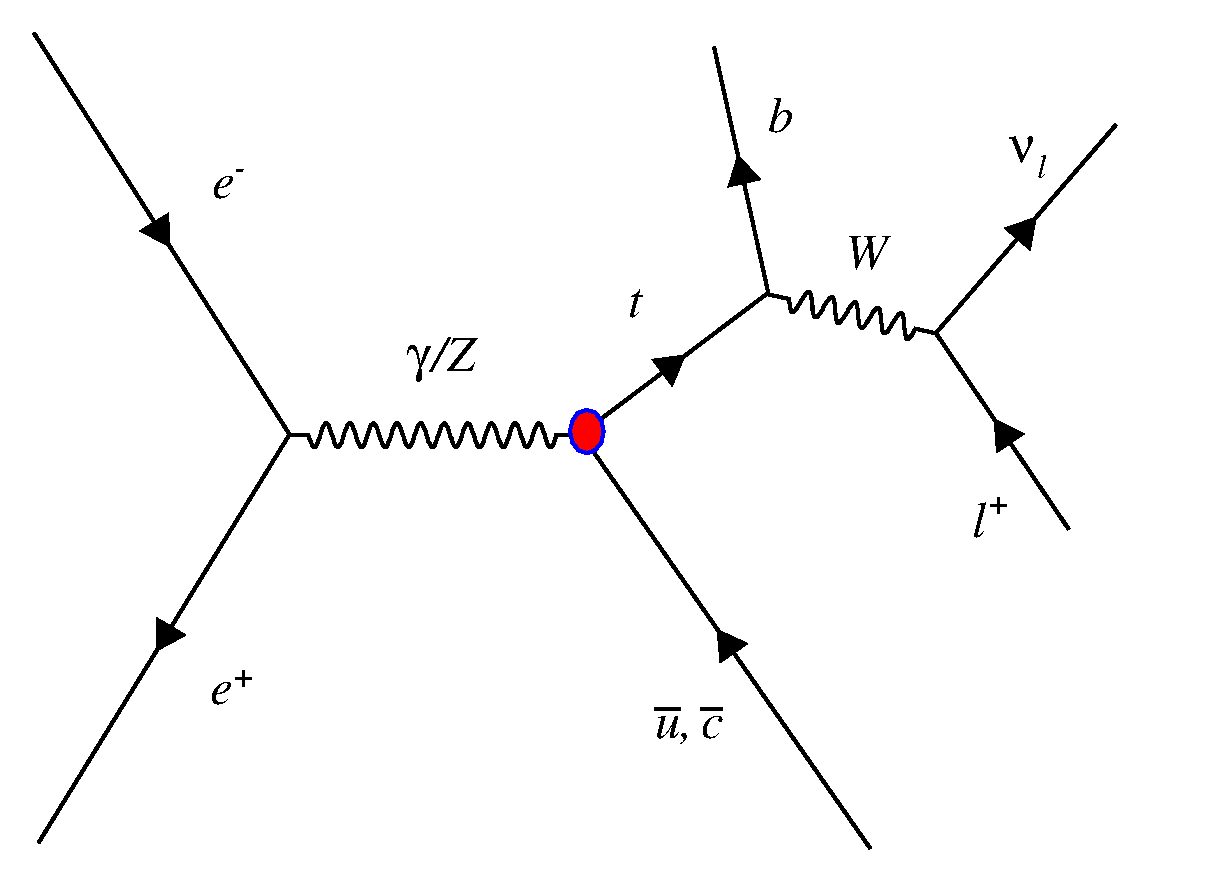
\includegraphics{images/feynman-diagram.eps}}
\end{center}
\caption{Representative leading-order Feynman diagrams for the production of 
top quark via FCNC in leptonic decay channel of the W-boson from top decay.}\label{Feyn-leptonic}
\end{figure}
%---------------------------


In the leptonic scenario (as shown in Fig.~\ref{Feyn-leptonic}), the top quark 
decays according to the Standard Model 
(SM) process, where $t \to W^+ b \to \ell^+ \nu_\ell b$ and $\bar{t} \to W^- \bar{b} \to \ell^- \overline{\nu}_\ell \bar{b}$. 
As a result, the final state comprises a charged lepton $\ell$, missing energy (neutrino), 
a $b$-jet, and a light jet, as depicted in Figure~\ref{Feyn-leptonic}.

%---------------------------
\begin{figure}
\begin{center}
\resizebox{0.4\textwidth}{!}{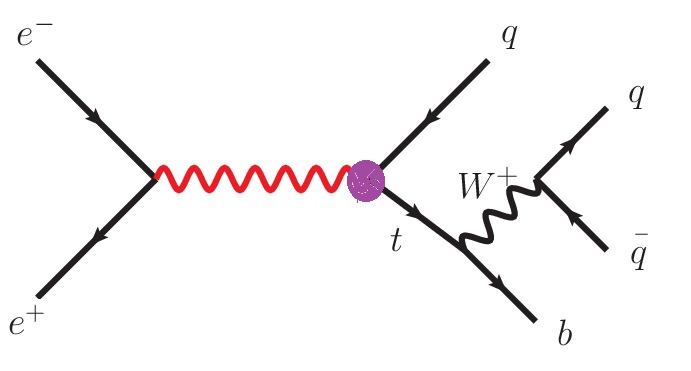
\includegraphics{images/full-hadronic.jpg}}
\end{center}
\caption{Representative leading order Feynman diagrams for the production of 
top quark via FCNC in a fully hadronic decay channel.}\label{Feyn-fully-hadronic}
\end{figure}
%---------------------------

In the fully hadronic scenario (as shown in Fig.~\ref{Feyn-fully-hadronic}), the 
top quark decays as $t \to W^+ b \to j j b$ 
and $\bar{t} \to W^- \bar{b} \to j j \bar{b}$, where $j$ represents a jet. Consequently, 
the final state consists of three jets plus an additional light jet, 
with at least one jet being identified as a b-tagged jet.

Further information regarding the analysis strategy and event selection will 
be provided in the subsequent sections.





%
%%%%%%%%%%%%%%%%%%%%%%%%%%%%%%%%%%%%%%%%%%%%%%%%%%%%%%%%%%%%%%%%%%%%%%%
\section{Theoretical framework}\label{Theoretical-Framework}
%%%%%%%%%%%%%%%%%%%%%%%%%%%%%%%%%%%%%%%%%%%%%%%%%%%%%%%%%%%%%%%%%%%%%%%
%


In this section, we outline the theoretical framework and assumptions utilized in 
our analysis to investigate the FCNC transitions of the top quark at the FCC-ee.

The possibility of the top quark anomalous FCNC couplings with light quarks $(q=u, c)$ and a 
gauge bosons (Z and $\gamma$) is explored in a 
model-independent way considering the 
most general effective Lagrangian approach~\cite{Aguilar-Saavedra:2004mfd,Aguilar-Saavedra:2008nuh}. 
In the search for anomalous FCNC interactions at high-energy colliders, this approach 
has been extensively studied in the literature for both the lepton and hadron colliders. 
In this framework, these FCNC vertices are described by higher-dimensional 
effective operators ${\cal L}_\text{FCNC}^{tqX}$ independently from the underlying theory. 
Up to dimension-six operators, the FCNC Lagrangian 
of the $tqg$, $tqH$, $t q Z (\sigma^{\mu \nu})$, 
$t q Z (\gamma_{\mu})$ and $tq\gamma$ 
interactions can be written as~\cite{Aguilar-Saavedra:2004mfd,Aguilar-Saavedra:2008nuh,Aguilar-Saavedra:2009ygx}

%--------------------------------
\begin{equation}
\label{Effective-Lagrangian}
\begin{split}
\mathcal{L}_{\text 
			{FCNC}}^{{tqX}} = &
		\ \sum_{q = u, c}
		\bigg[
		\frac{g_{s}}{2 m_t}
		\bar{q} \lambda^a
		\sigma^{{\mu} {\nu}} \,
		(\zeta_{qt}^L P^L
		+  \zeta_{qt}^R P^R) \, 
		t G^a_{{\mu} {\nu}} - \frac{1}{\sqrt{2}}
		\bar{q} \, (\eta_{qt}^L P^L
		+ \eta_{qt}^R P^R) \, t H   \\
		&\ + \frac{g_W}{4 c_W m_Z}
		\bar{q} \sigma^{{\mu} {\nu}} \,
		(\kappa_{qt}^L P_L
		+  \kappa_{qt}^R P_R)
		\, t Z_{{\mu} {\nu}}  - \frac{g_W}{2 c_W} \bar{q}
		\gamma^{\mu} \, (X_{qt}^L P_L +
		X_{qt}^R P_R) \, t Z_{\mu}   \\
		&\ + \frac{e}{2 m_t} \bar{q}
		\sigma^{{\mu} {\nu}} \,
		(\lambda_{qt}^L P_L
		+  \lambda_{qt}^R P_R) \,
		t A_{{\mu} {\nu}}  \bigg]
		+ \text{h.c.} \,.
\end{split}
\end{equation}
%--------------------------------

In Eq.~\eqref{Effective-Lagrangian}, the dimensionless parameters $\zeta_{qt}$, 
$\eta_{qt}$, $\kappa_{qt}$, $X_{qt}$ and $\lambda_{qt}$ represent the 
strength of the FCNC 
interactions of a top quark with gluon, Higgs, $Z$, and $\gamma$, respectively. 
In the above equation, $q$ indicates an up or charm quark as well.
In this work, we mainly concentrate on the case of top quark FCNC
couplings $tq\gamma$ and  $tqZ$ at FCCee.
At the tree level in the SM, all the above coefficients are zero.
In the presence of anomalous FCNC vertices, the straightforward way is to 
set limits on these coupling's strengths and then translate them to the  
corresponding branching fractions. 
In the above equation, $g_s$ is the strong coupling constant, 
and $P_{L}$ and  $P_{R}$  denote 
the left- and right-handed projection operators. 
In this study, we assume no specific chirality 
for the anomalous FCNC interactions, and hence, one could 
set $\kappa_{qt}^{L} =  \kappa_{qt}^{R} = \kappa_{qt}$,  
$X_{qt}^{L} =  X_{qt}^{R} = X_{qt}$  and $\lambda_{qt}^{L} =  \lambda_{qt}^{R} = \lambda_{qt}$. 
As we mentioned earlier in the introduction, 
the single top FCNC signal includes the $Z$ and $\gamma$ top quark FCNC 
interactions, and hence, make it possible to study all the coefficients 
sensitive to the $tq\gamma$ and  $tqZ$.

We should notice here that, the fixed values of
$\kappa_{qt} = 0.1$ and $\lambda_{qt} = 0.1$ with
$q = u$ and $c$ are chosen for all coupling strengths as the 
benchmark point if not stated otherwise. 
Taking these typical
benchmarks input for the top FCNC signal, the expected
cross sections are calculated.




%
%%%%%%%%%%%%%%%%%%%%%%%%%%%%%%%%%%%%%%%%%%%%%%%%%%%%%%%%%%%%%%%%%%%%%%%
\section{simulated samples}\label{sec:strategy}
%%%%%%%%%%%%%%%%%%%%%%%%%%%%%%%%%%%%%%%%%%%%%%%%%%%%%%%%%%%%%%%%%%%%%%%
The analysis is based on the benchmarks introduces in the Future circular collider (FCC) conceptual design  in electron-positron collisions at center of mass energy $240 $GeV and $365$ GeV corresponding to the integrated luminosity of 5$\inab$ and 1.5$\inab$, respectively. 

The FCC-ee, a proposed high-energy frontier electron-positron collider, holds immense potential for precision measurements in the field of particle physics.
In order to capture a wide range of physical processes, events are generated  by using various generators. To simulate the response of the detector and reconstruct the events, fast simulation package DELPHES \cite{} is used. DELPHES applies a resolution formula and efficiency to smear the particles generated at the generator level, thus emulating the characteristics of a realistic detector. This complete chain of event generation, simulation, and reconstruction is seamlessly integrated within the Key4HEP software framework. For our analysis, we utilize the official central samples from the Spring2021 campaign, ensuring the reliability and consistency of our results.
\par
The Innovative Detector for an Electron-positron Accelerator (IDEA) is a cutting-edge detector concept designed for future electron-positron colliders like the FCC-ee. It incorporates advanced technologies and design features to achieve exceptional performance in precision measurements, particle identification, and energy resolution. The IDEA detector includes components such as a high-resolution tracking system, electromagnetic and hadronic calorimeters, advanced particle identification techniques, a magnet system for precise momentum measurement, and forward/backward detectors for comprehensive coverage. The design focuses on optimizing energy and spatial resolution, particle identification efficiency, and overall detector performance across a wide range of particle energies.
%%%%%%%%%%%%%%%%%%%%%%%%%%%%%%%%%%%%%%%%%%%%%%%%%%
\subsection{simulated signal samples}\label{sec:MC-samp}
%%%%%%%%%%%%%%%%%%%%%%%%%%%%%%%%%%%%%%%%%%%%%%%%%%

In order to generate the signal events, the FCNC lagrangian introduced in the Eq\ref{Effective-Lagrangian}, is implemented into the {\sc MadGraph5\_aMC@NLO} event generator by using the  {\tt FeynRules} package and the corresponding UFO file.  The signal comprises single top production where the FCNC couplings appear at the production level of $e^-e+ \rightarrow t q$.  In presented cross-sections in the Table \ref{MCsample}, coupling strengths $\lambda_{tq\gamma}$ and $\kappa_{tqZ}$ are left free letting only one of them to be non-zero at a time. All samples are generated at leading order (LO).
%%%%%%%%%%%%%%%%%%%%%%%%%%%%%%%%%%%%%%%%%%%%%%%%%%
\subsection{Simulated background samples}\label{sec:MC-samp}
%%%%%%%%%%%%%%%%%%%%%%%%%%%%%%%%%%%%%%%%%%%%%%%%%%
In order to estimate the contributions of background processes, {\tt MadGraph5\_aMC@NLO}, the {\tt WHIZARD} event generator and parton showering with {\tt PYTHIA6}, and both generation and parton showering with {\tt PYTHIA8} MC generator is used.   

\begin{table}[htbp]
\resizebox{\columnwidth}{!}{%
	\begin{tabular}{c c c c c}
       \hline
		MC sample name ~~&Generator&Processes &~~x-section at 240 GeV [pb]~~&~~x-section at 365 GeV [pb]\\ \hline
  {\bf signal} &&&&\\
		${\tt mgp8\_ee\_tbw\_FCNC\_tua}$ &{\tt MadGraph5\_aMC@NLO }&$e^-e^+\rightarrow tu$ &  (LO)&\\
        ${\tt mgp8\_ee\_tbw\_FCNC\_tca}$&{\tt MadGraph5\_aMC@NLO } &$e^-e^+\rightarrow tc$&&\\
        ${\tt mgp8\_ee\_tbw\_FCNC\_tuz}$&{\tt MadGraph5\_aMC@NLO } &$e^-e^+\rightarrow tu$&&\\
        ${\tt mgp8\_ee\_tbw\_FCNC\_tcz}$&{\tt MadGraph5\_aMC@NLO }&$e^-e^+\rightarrow tc$&&\\
        \hline
         {\bf background} &&&&\\
        ${\tt p8\_ee\_ZH}$&{\tt PYTHIA8}&$e^-e^+\rightarrow ZH$&202 &117\\
       $ {\tt p8\_ee\_WW}$&{\tt PYTHIA8}&$e^-e^+\rightarrow W^+W^-$&16439&10717\\
       $ {\tt p8\_ee\_ZZ}$&{\tt PYTHIA8}&$e^-e^+\rightarrow ZZ$&1360&643 \\
       ${\tt wzp6\_egamma\_tbnu}$&{\tt WHIZARD+PYTHIA6}&$e^+\gamma \rightarrow tb\nu$&0.01 &0.2 \\
       ${\tt wzp6\_egamma\_eZ\_Zbb}$&{\tt WHIZARD+PYTHIA6}& $e^-\gamma \rightarrow Zbb$&\\
       ${\tt wzp6\_egamma\_eZ\_Zqq}$&{\tt WHIZARD+PYTHIA6}&$e^-\gamma \rightarrow Zqq$&& \\
       ${\tt wzp6\_ee\_tbjj\_singleTop}$&{\tt WHIZARD+PYTHIA6}& $e^-e^+ \rightarrow Zqq$& -&6\\
       ${\tt p8\_ee\_tt}$&{\tt PYTHIA8}&$e^-e^+ \rightarrow t\bar{t}$& -&800\\
		%	$/\text{WGToLNuG}\_\text{TuneCP5}\_\text{13TeV-madgraphMLM-pythia8}/\text{RunIISummer20UL17NanoAODv9-106X}\_\text{mc2017}\_\text{realistic}\_\text{v9-v1}$ & 191.50  (LO)\\ \hline
  
		\end{tabular}
  }
  
\caption{MC samples used in this analysis in $240\GeV$ and $365\GeV$ center-of-mass-energy}
\label{MCsample}

\end{table}

%%%%%%%%%%%%%%%%%%%%%%%%%%%%%%%%%%%%%%%%%%%%%%%%%%%%%%%%%%%%%%%%%%%%%%%
\section{Analysis strategy and event selection}\label{sec:strategy}
%%%%%%%%%%%%%%%%%%%%%%%%%%%%%%%%%%%%%%%%%%%%%%%%%%%%%%%%%%%%%%%%%%%%%%%
%
We conduct our analysis in a model-independent manner, utilizing the effective Lagrangian approach described in Equation~\eqref{Effective-Lagrangian}. Our study focuses on the future collider FCC-ee, operating at center-of-mass energies of $\sqrt{s}$ = 240 GeV and 365 GeV. In our analysis, we consider both the leptonic (electron and muon) and fully hadronic decays of the $W$ boson in the top quark decay.
To perform our analysis, we utilize centrally produced samples within the FCCSW framework. These samples incorporate an {\tt IDEA} detector response to accurately model the detector effects. We also take into account all major background contributions and thoroughly analyze them.
For the discrimination of signals from background processes, we propose a set of kinematic variables as input variables. The specific details of the event selection criteria and kinematic variables will be presented in the following sections. We begin by discussing the leptonic decay channel, followed by a comprehensive presentation of the fully hadronic analysis.
%
%%%%%%%%%%%%%%%%%%%%%%%%%%%%%%%%%%%%%%%%%%%%%%%%%%%%%%%%%%%%%%%%%%%%%%%
\subsection{Leptonic decay channel}\label{Leptonic-decay-channel}
%%%%%%%%%%%%%%%%%%%%%%%%%%%%%%%%%%%%%%%%%%%%%%%%%%%%%%%%%%%%%%%%%%%%%%%
%

For the analysis of leptonic decay, the signal process is defined as electron-positron annihilation into a Z or photon, which then decays into a top quark and an up or charm quark, along with their antiparticles. The top quark subsequently decays through the Standard Model, producing a W boson and a bottom quark, which further decay into a charged lepton (either an electron or a muon), a corresponding neutrino, and a bottom quark (or its antiparticle). Therefore, the final state consists of a charged lepton, missing energy, a bottom quark, and a light quark. We conduct this analysis separately for muons and electrons.
We evaluated various jet clustering algorithms provided in the official framework and ultimately selected the {\tt ee-$k_T$ Durham} jet clustering algorithm ~\cite{Catani:1991hj, Lai:2021rko} with the Energy recombination scheme (ES) ~\cite{Tenchini}. Since the final state involves two jets, we specifically consider the exclusive mode with exactly two jets. In the case of the {\tt ee-$k_T$ Durham}  algorithm, our final results are based on the implementation {\tt JetClustering::clustering\_ee\_kt(2, 2, 1, 0)} available in the official FCCAnalysis framework. The first argument in {\tt JetClustering::clustering\_ee\_kt} denotes the exclusive clustering, specifying the number of the event clustered into exactly n-jets. The second argument indicates exactly two jets in the final state. The third argument determines the ordering of jets based on energy, and the last argument corresponds to the E recombination scheme ~\cite{Tenchini}.

Based on the expected signature of the signal process, the 
main background contributing to the signal 240 GeV center-of-mass energy includes the
$e^- e^+ \rightarrow WW$, $e^- e^+ \rightarrow HZ$, $e^- e^+ \rightarrow ZZ$,
$e^- e^+ \rightarrow tq$, $e^- e^+ \rightarrow eebb$ and $e^- e^+ \rightarrow eeqq \, (q=u, d, s)$.
For the case of 365 GeV center-of-mass energy, in addition to the list mentioned above, the single top 
production $e^- e^+ \rightarrow tbjj$ and top-pair production $e^- e^+ \rightarrow t\bar{t}$ will also contribute. 

These officially generated signal samples include:

\begin{itemize}
\item  {\tt p8\_ee\_ZH\_ecm240}
\item  {\tt p8\_ee\_WW\_ecm240}
\item  {\tt p8\_ee\_ZZ\_ecm240}
\item  {\tt wzp6\_egamma\_tbnu\_ecm240}
\item  {\tt wzp6\_gammae\_tbnu\_ecm240}
\item  {\tt wzp6\_egamma\_eZ\_Zbb\_ecm240}
\item  {\tt wzp6\_gammae\_eZ\_Zbb\_ecm240}
\item  {\tt wzp6\_egamma\_eZ\_Zqq\_ecm240}
\item  {\tt wzp6\_gammae\_eZ\_Zqq\_ecm240}
\end{itemize}
and the same notation for the 365 GeV, but this time  
{\tt wzp6\_ee\_tbjj\_singleTop\_ecm365} and {\tt p8\_ee\_tt\_ecm365} are also included.

To select events in this study, we impose certain criteria. Specifically, we only consider events that have a single charged lepton (either an electron or a muon) with a total momentum of at least 10 GeV and a polar angle greater than 13 degrees. Additionally, we require the presence of exactly two jets, each with a momentum of at least 20 GeV and a polar angle greater than 13 degrees. Furthermore, one of these jets must be identified as a $b$-quark jet.
To determine the most suitable jet clustering algorithm, we reconstruct the invariant mass distribution of the top quark using different algorithms. The corresponding plot, along with the momentum of the $b$ jet candidate, is displayed in Figure~\ref{diff-alg}.

%------------------------------------------------
\begin{figure*}[htb]
\vspace{0.50cm}
\centering
\subfloat{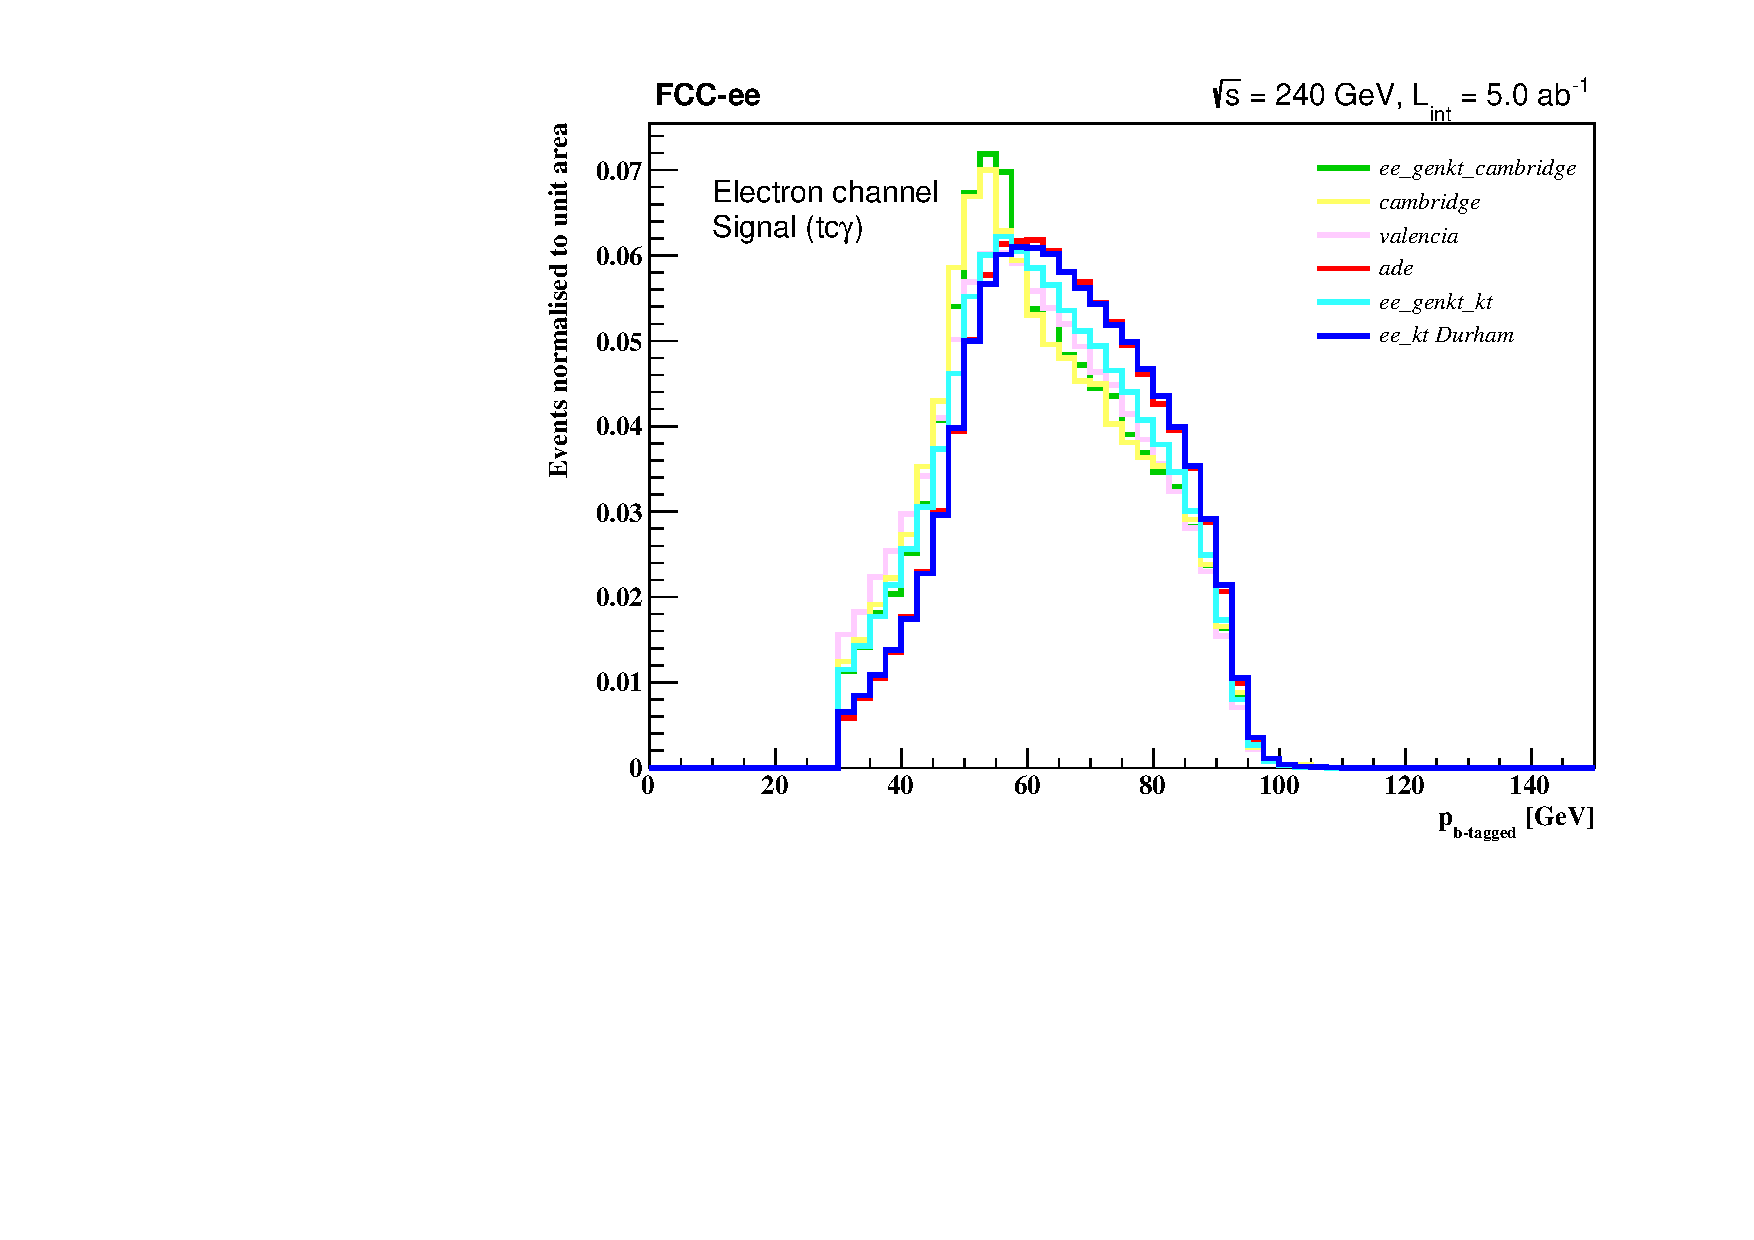
\includegraphics[width=0.45\textwidth]{Jet-Algorithm/pbjet-JetAlg-240GeV-leptonic.pdf}} 	
\subfloat{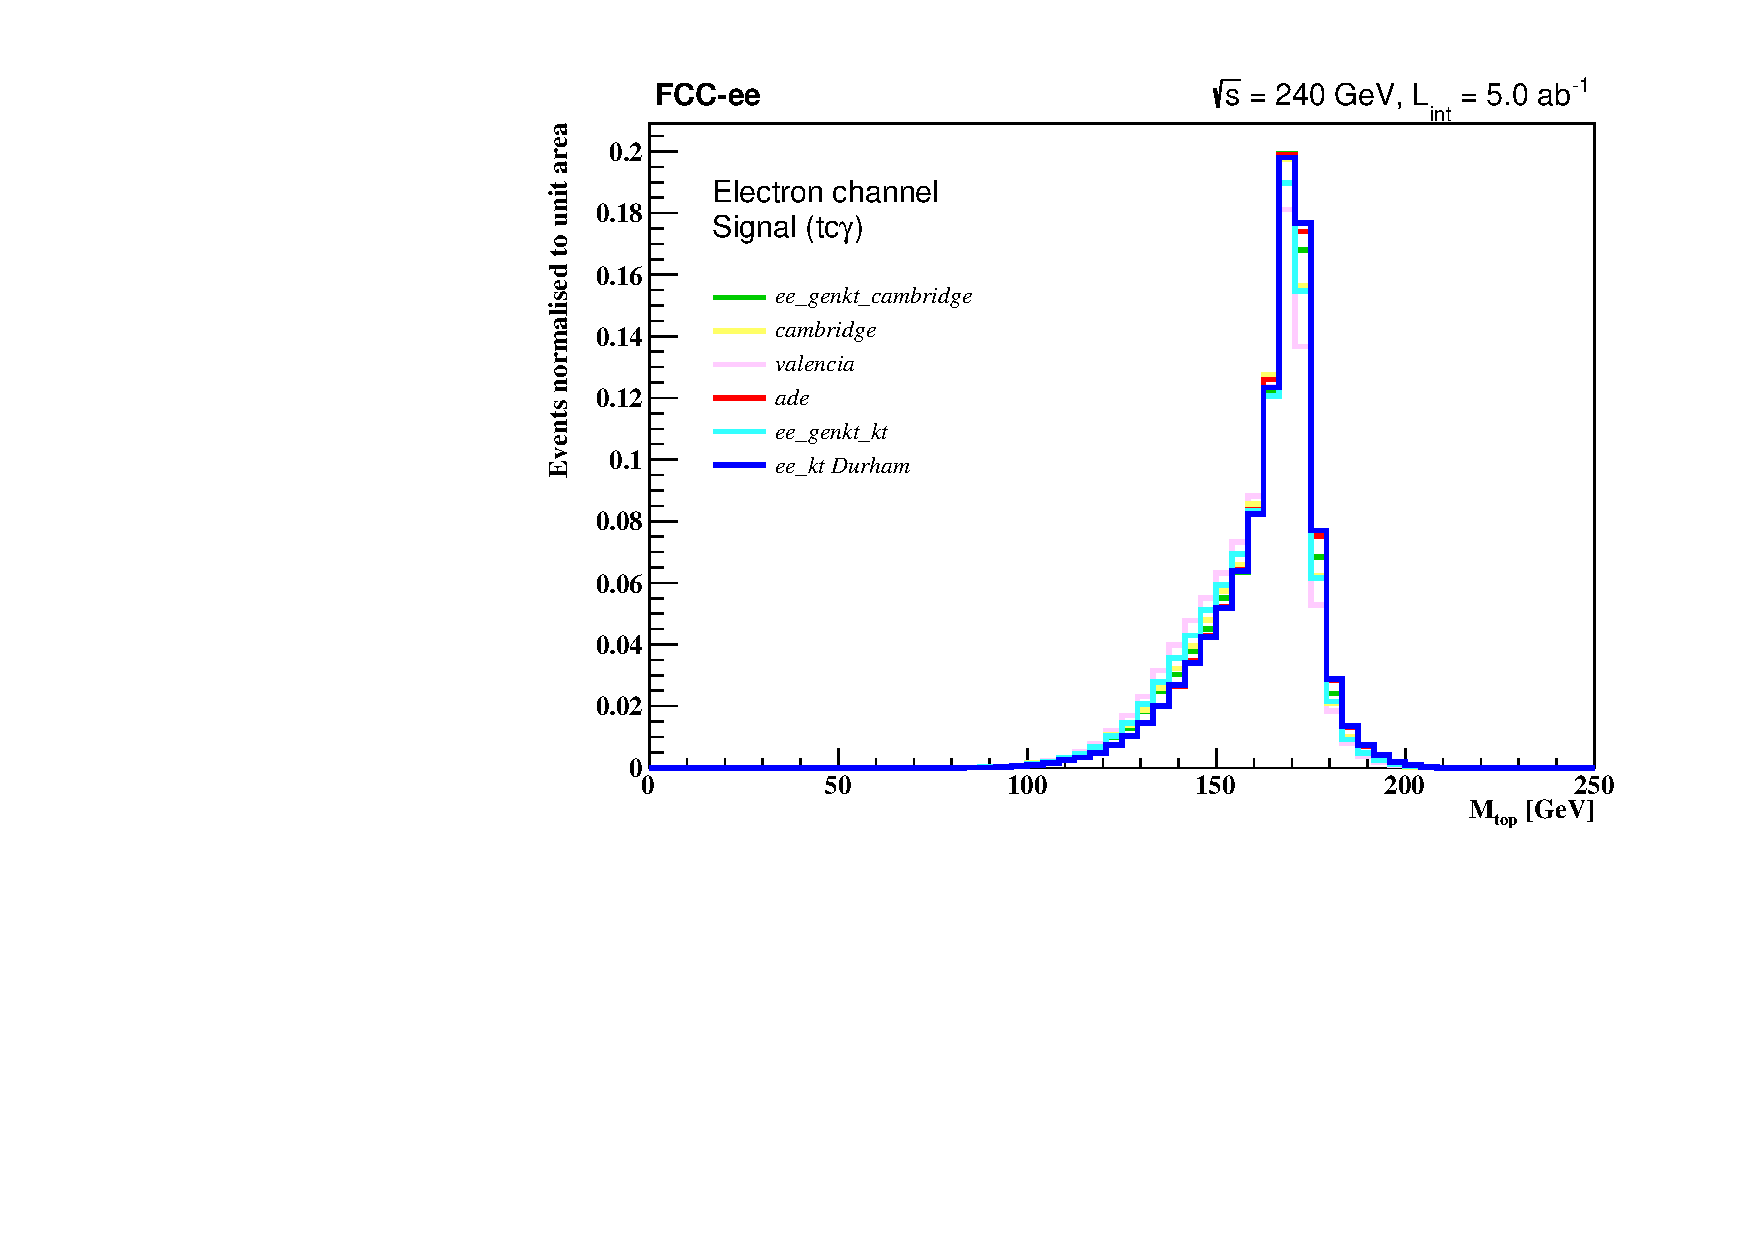
\includegraphics[width=0.45\textwidth]{Jet-Algorithm/topmass-JetAlg-240GeV-leptonic.pdf}}	
%\vspace{-6cm}
\begin{center}
\caption{ \small 
The mass distribution of the reconstructed top quark 
and the momentum of $b$ jet candidate for $t c\gamma$ signal for  
different jet clustering algorithms. The distributions are shown for the 
electron channel and center-of-mass energy of 240 GeV. }
\label{diff-alg}
\end{center}
\end{figure*}
%------------------------------------------------
As previously mentioned, we focus on the {\tt ee-kt Durham} jet clustering algorithm, specifically in conjunction with the {\tt ES} recombination scheme in exclusive mode. Using this combination, we analyze the mass distribution of the reconstructed top quark and the W boson for the $tc\gamma$ signal, as well as the main backgrounds. The corresponding results obtained using the {\tt ee-kt Durham} jet clustering algorithm are presented in Figures~\ref{W-top-mass-240GeV-leptonic} and \ref{W-top-365GeV-leptonic} for center-of-mass energies of 240 GeV and 365 GeV, respectively.

%------------------------------------------------
\begin{figure*}[htb]
\vspace{0.50cm}
\centering
\subfloat{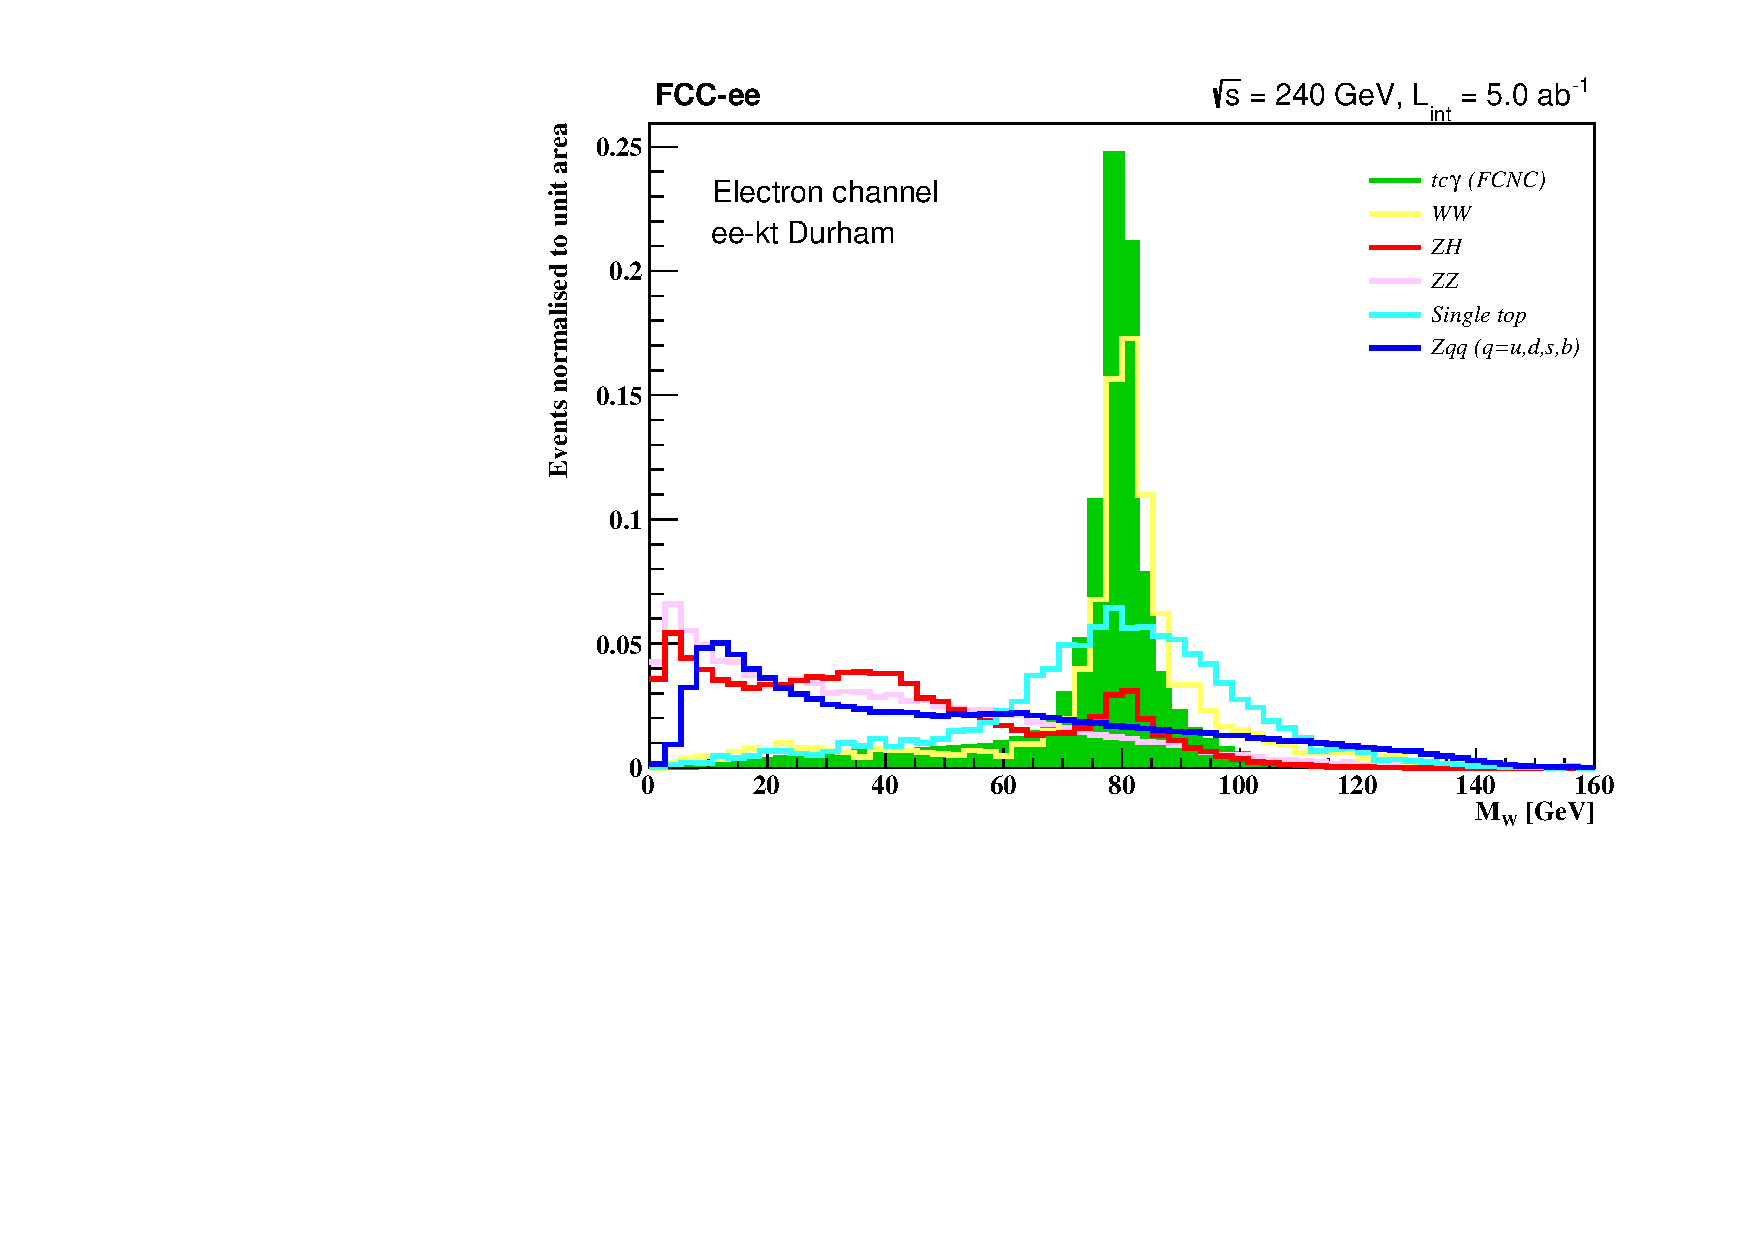
\includegraphics[width=0.45\textwidth]{240GeV-leptonic/Wmass-240GeV-leptonic.pdf}} 	
\subfloat{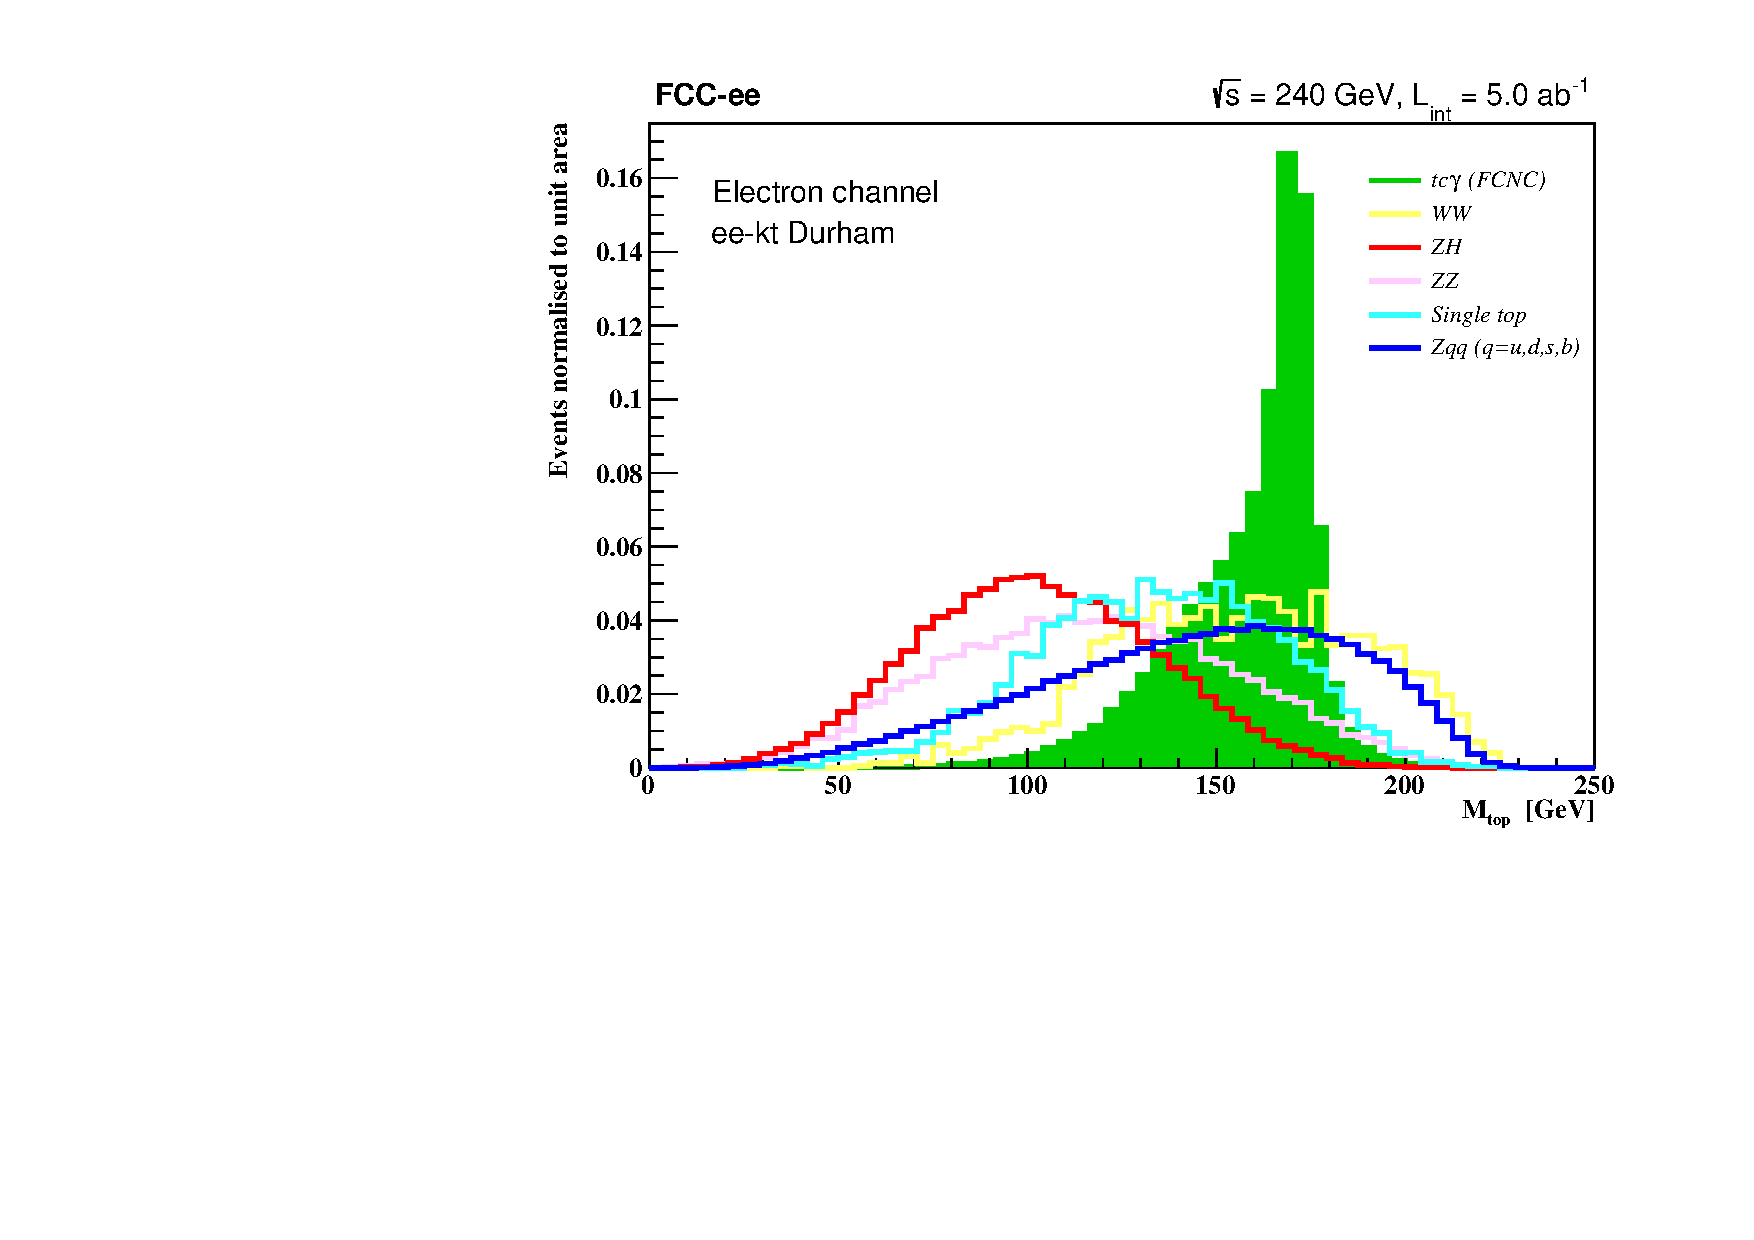
\includegraphics[width=0.45\textwidth]{240GeV-leptonic/topmass-240GeV-leptonic.pdf}}	
%\vspace{-6cm}
\begin{center}
\caption{ \small 
The mass distribution of the reconstructed top quark 
and the W boson for $tc\gamma$ signal and main backgrounds  
using the {\tt ee-kt Durham} jet clustering algorithm and for 
the center-of-mass energy of 240 GeV. }
\label{W-top-mass-240GeV-leptonic}
\end{center}
\end{figure*}
%------------------------------------------------





%------------------------------------------------
\begin{figure*}[htb]
\vspace{0.50cm}
\centering
\subfloat{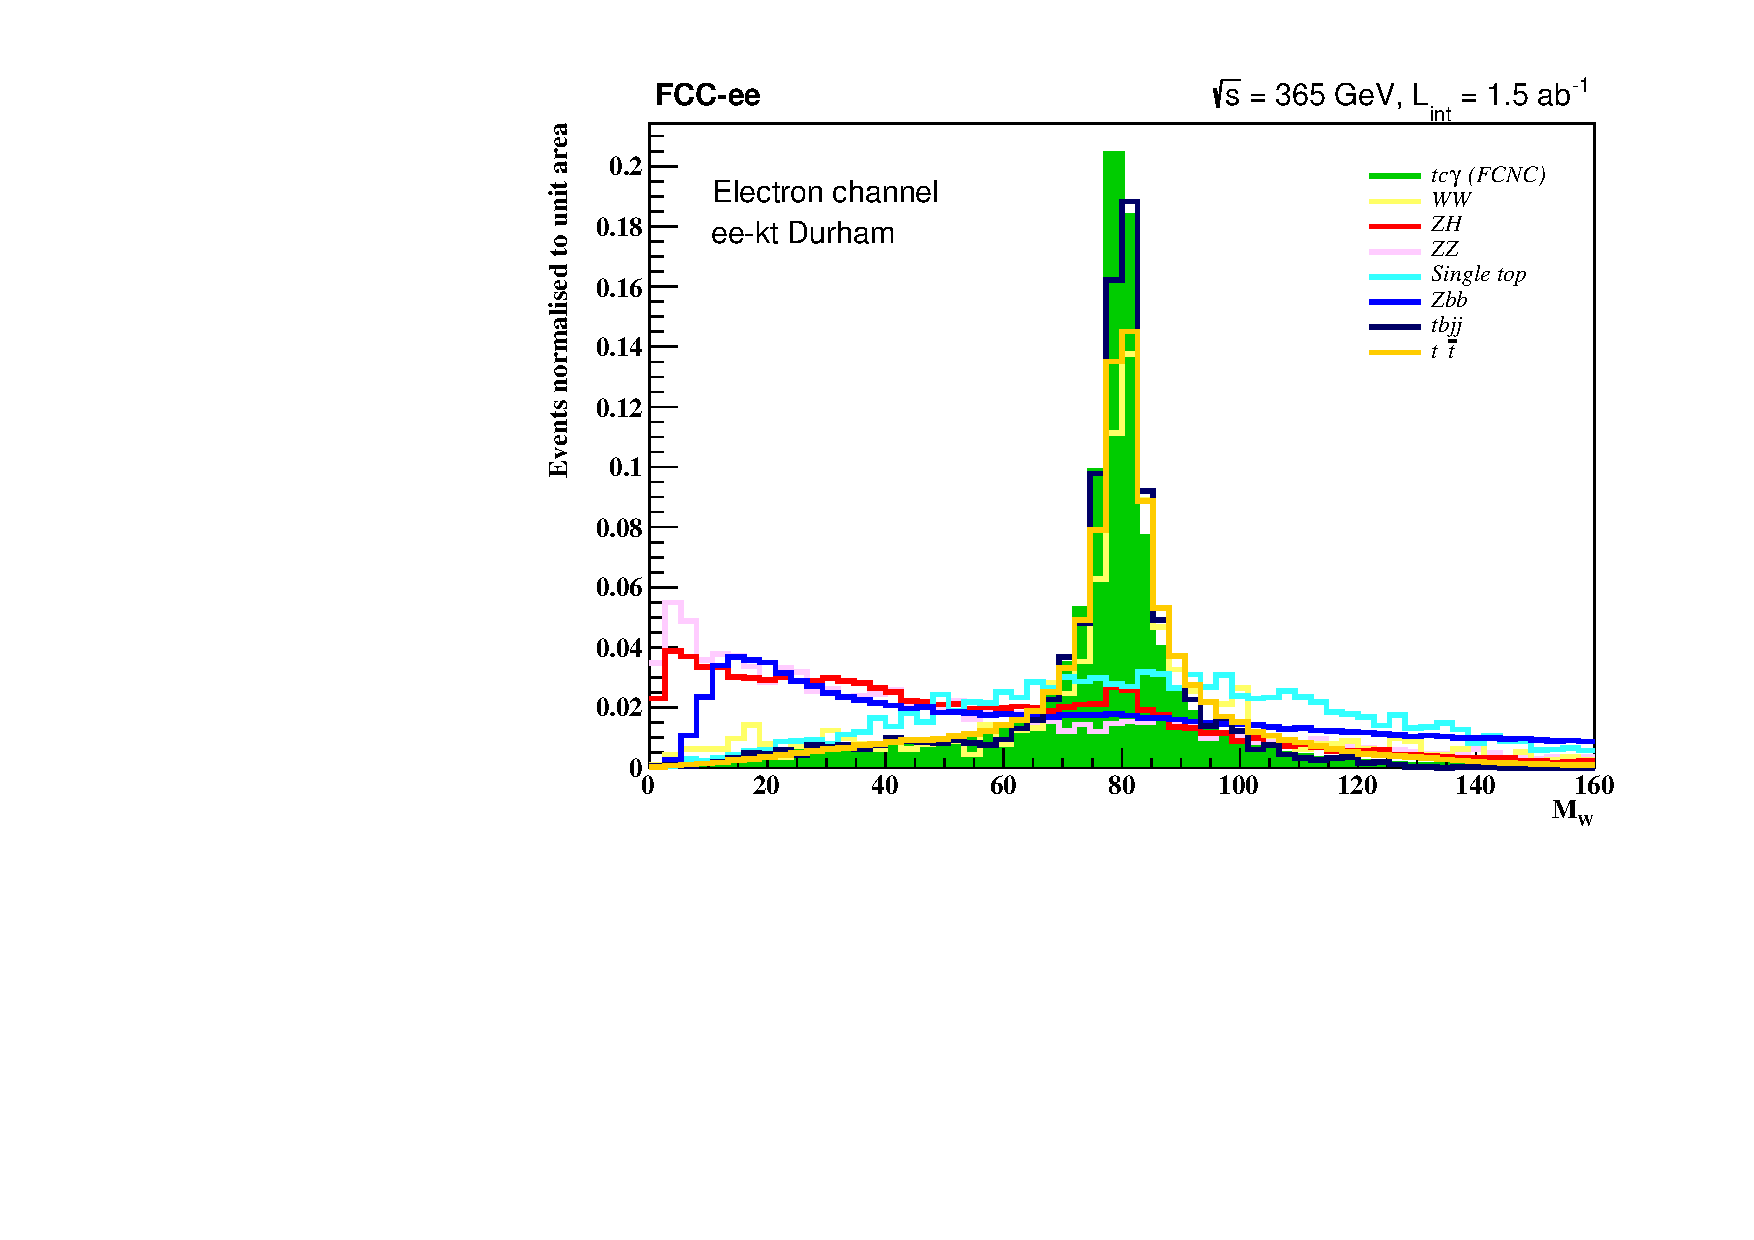
\includegraphics[width=0.45\textwidth]{365GeV-leptonic/Wmass-365GeV-leptonic.pdf}} 	
\subfloat{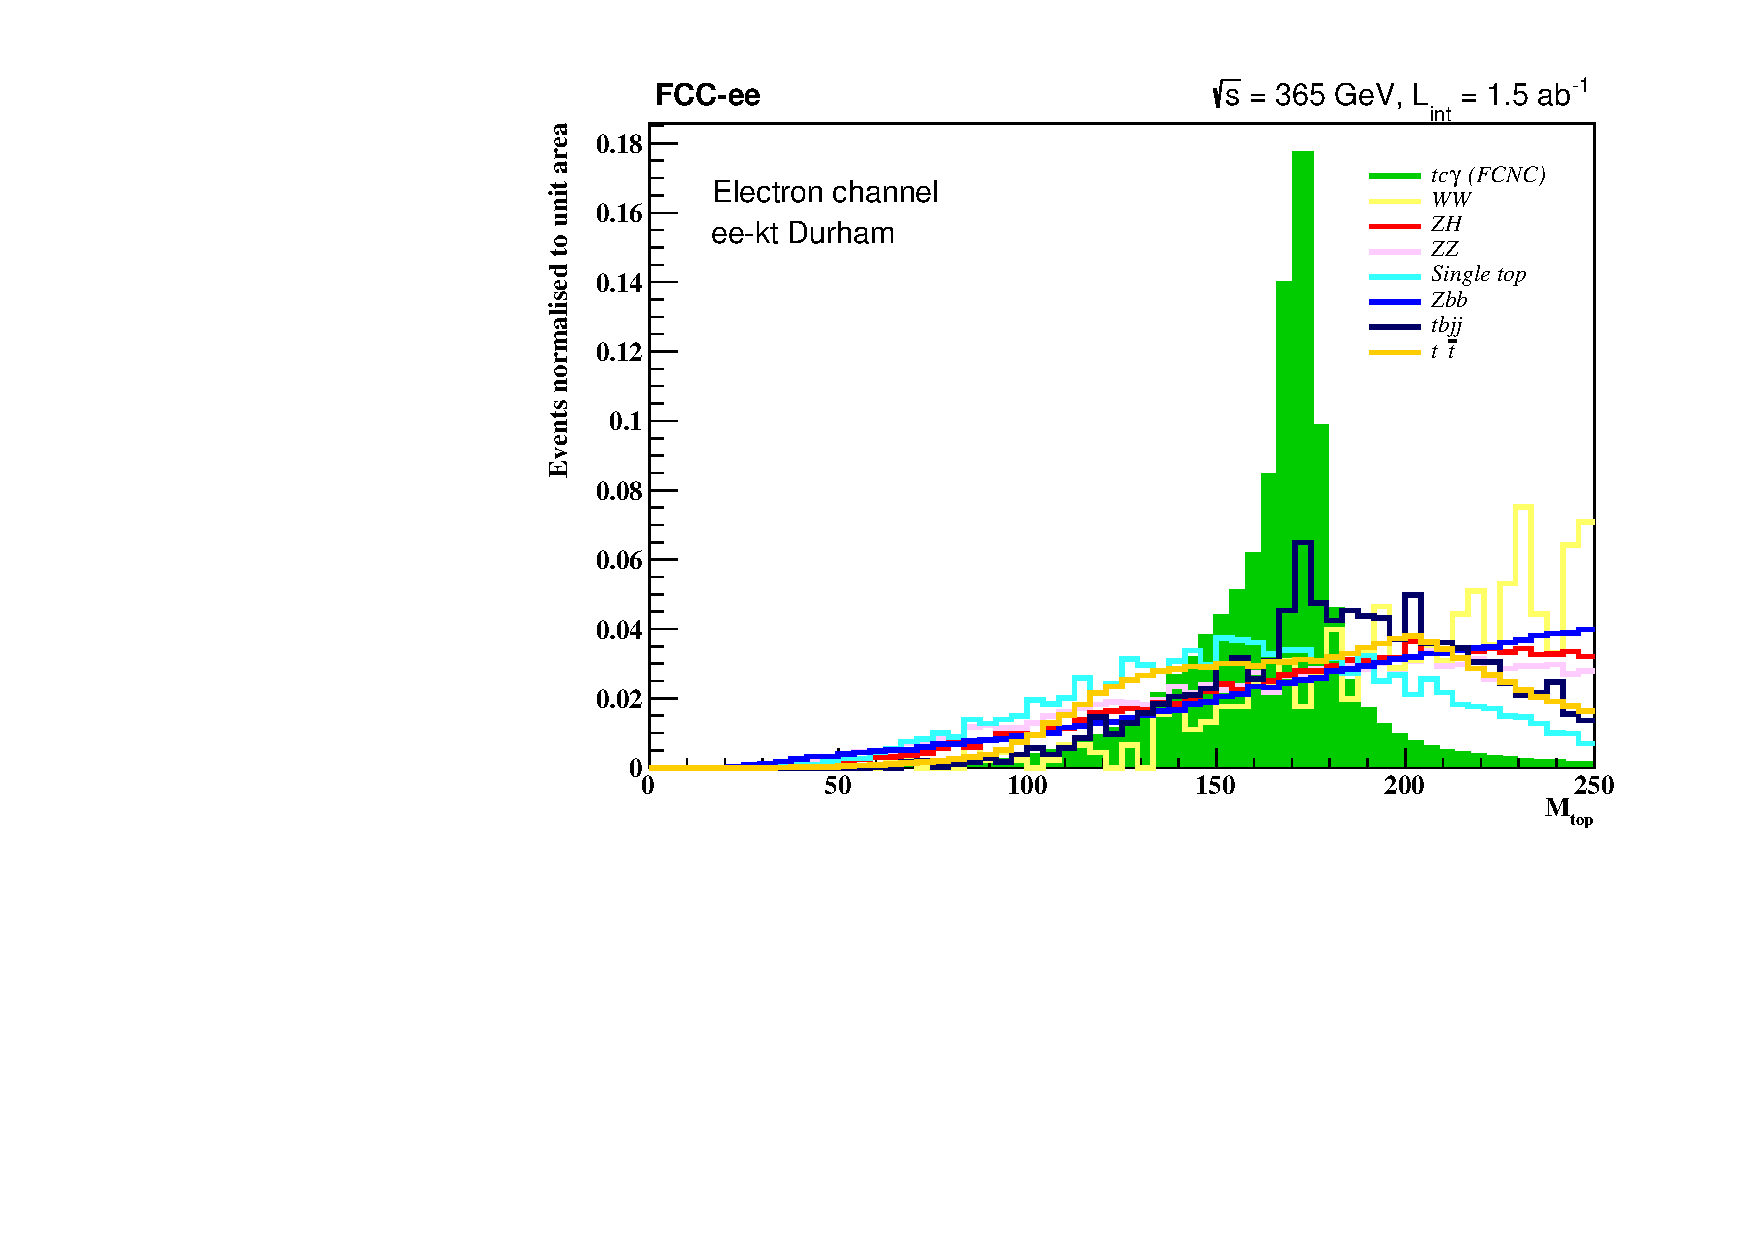
\includegraphics[width=0.45\textwidth]{365GeV-leptonic/topmass-365GeV-leptonic.pdf}}	
%\vspace{-6cm}
\begin{center}
\caption{ \small 
The mass distribution of the reconstructed top quark 
and the W boson for $tc\gamma$ signal and main backgrounds  
using the {\tt ee-kt Durham} jet clustering algorithm and for 
the center-of-mass energy of 365 GeV. }
\label{W-top-365GeV-leptonic}
\end{center}
\end{figure*}
%------------------------------------------------

In order to distinguish between signal and background processes effectively, we carefully select variables with the highest discrimination power. The distributions of some of these selected variables are displayed in Figure~\ref{variables-1}. These distributions correspond to the signal scenario with an anomalous $tc\gamma$ coupling in the electron channel at a center-of-mass energy of 240 GeV. It is worth noting that the same variables are utilized to differentiate the signal from backgrounds in all signal scenarios involving $tc\gamma$ and $tcZ$.
The analyses are conducted separately for the electron and muon channels, as well as for different light quark flavors such as $c$ and $u$, at center-of-mass energies of both 240 GeV and 365 GeV, while employing the same set of variables.

%------------------------------------------------
\begin{figure*}[htb]
\vspace{0.50cm}
\centering
\subfloat{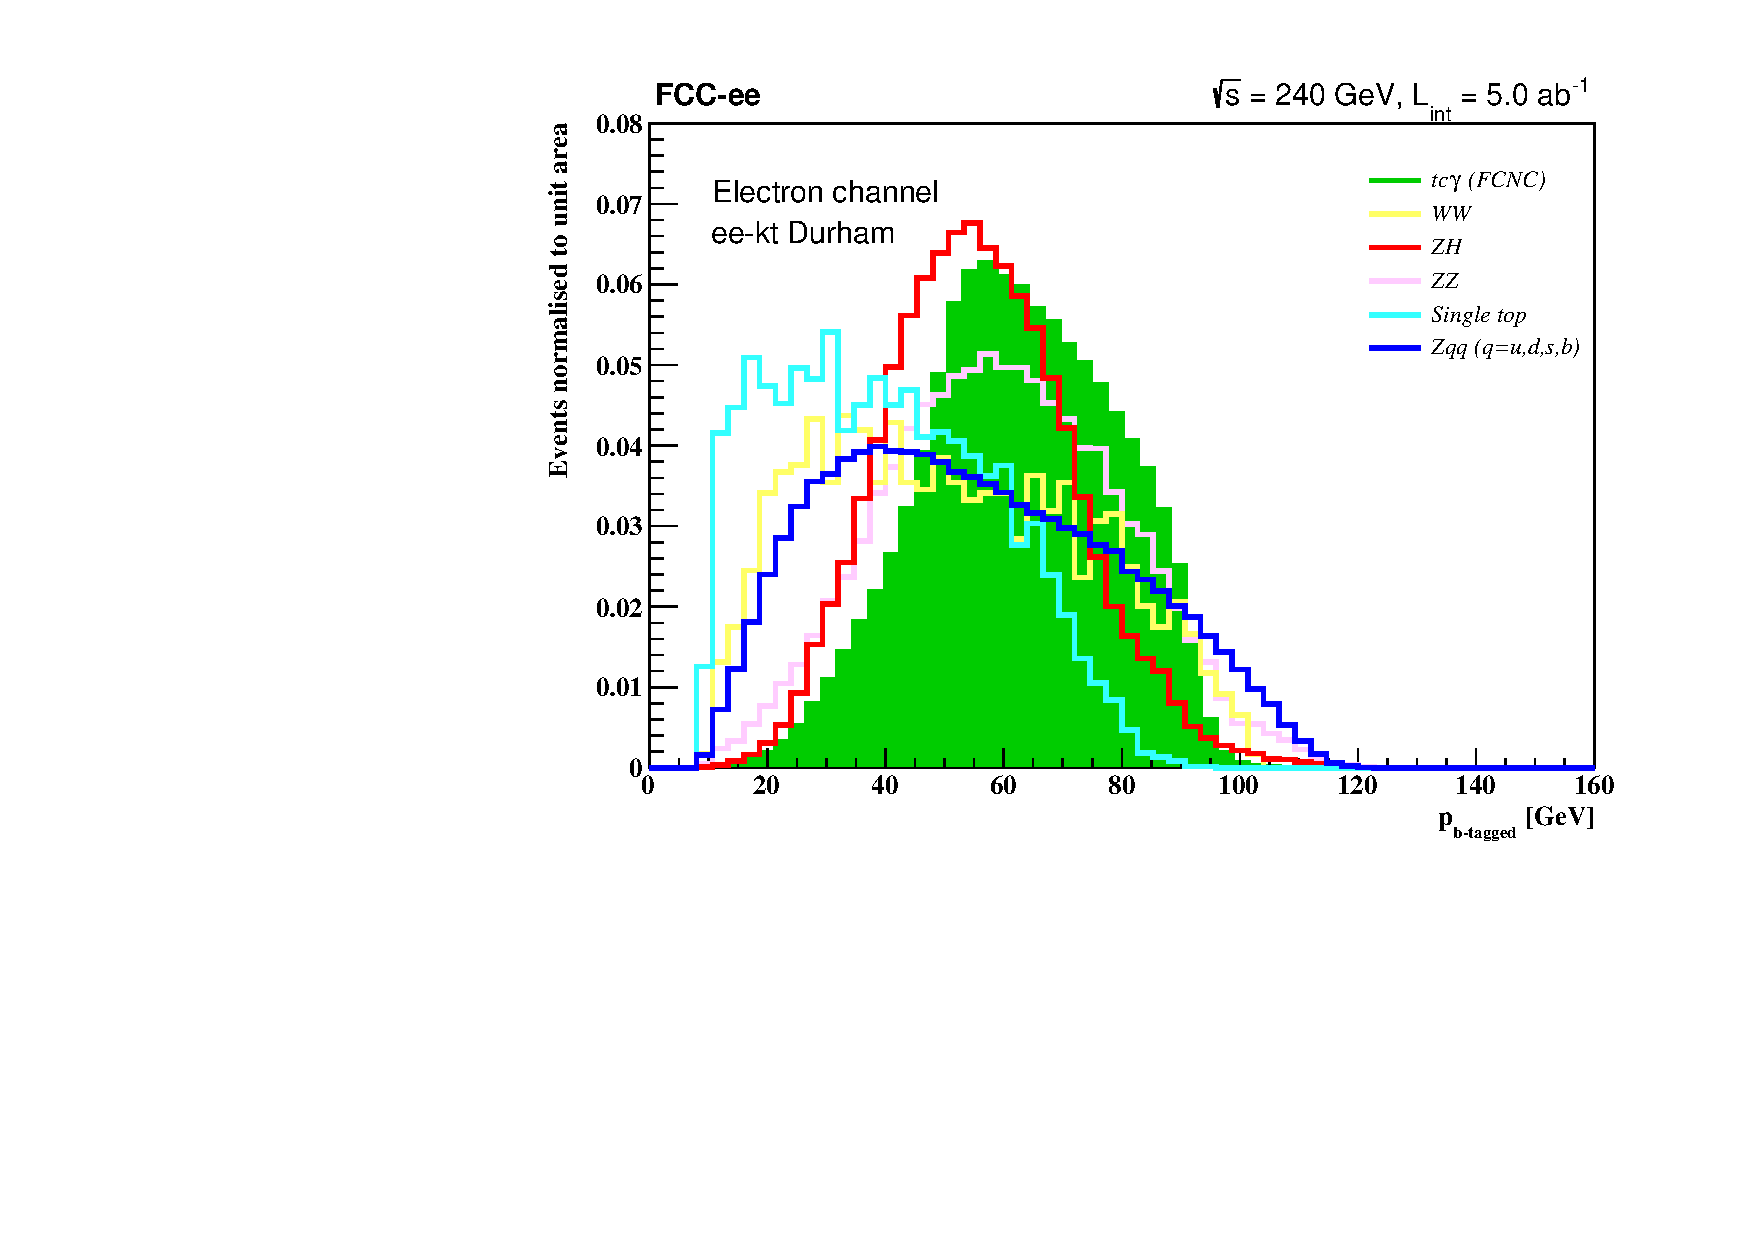
\includegraphics[width=0.45\textwidth]{240GeV-leptonic/pbjet-240GeV-leptonic.pdf}} 	
\subfloat{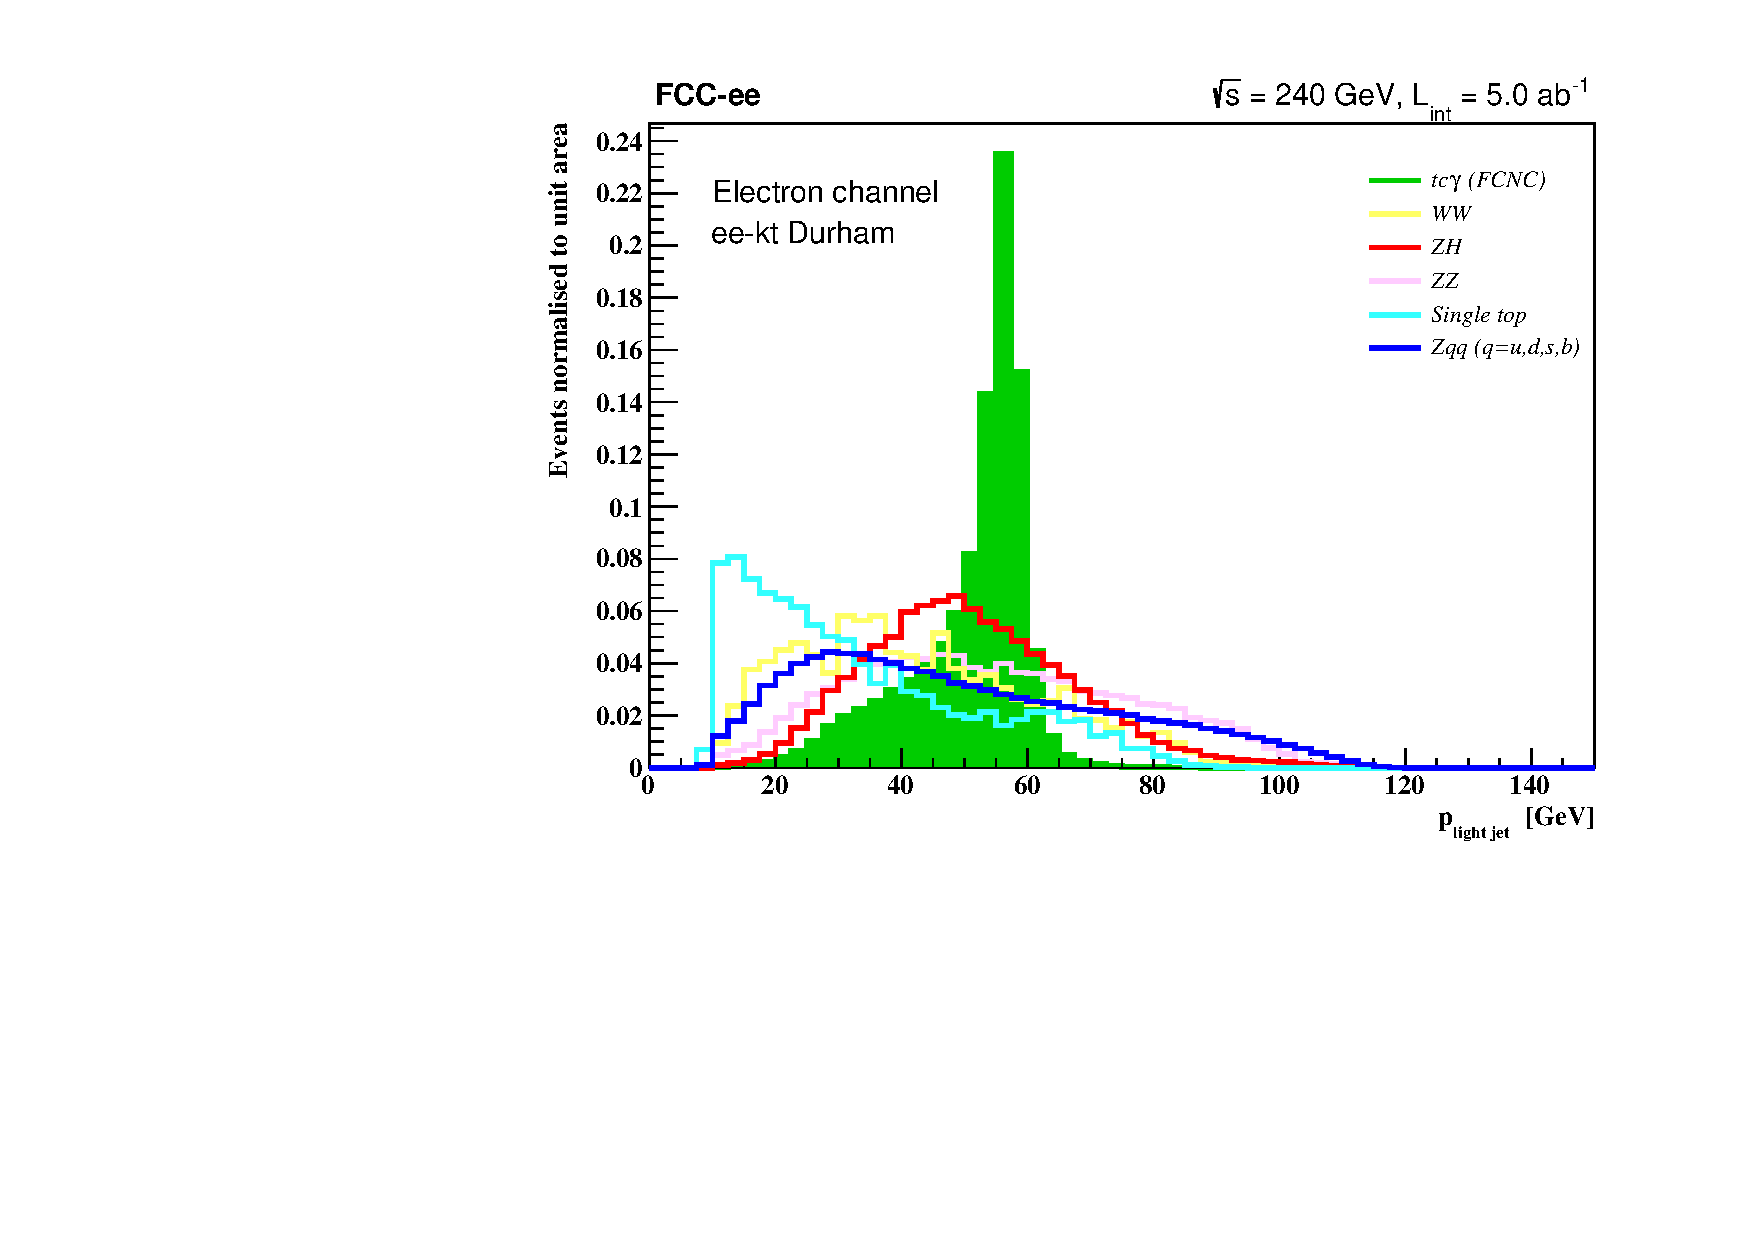
\includegraphics[width=0.45\textwidth]{240GeV-leptonic/plightjet-240GeV-leptonic.pdf}} \\
\subfloat{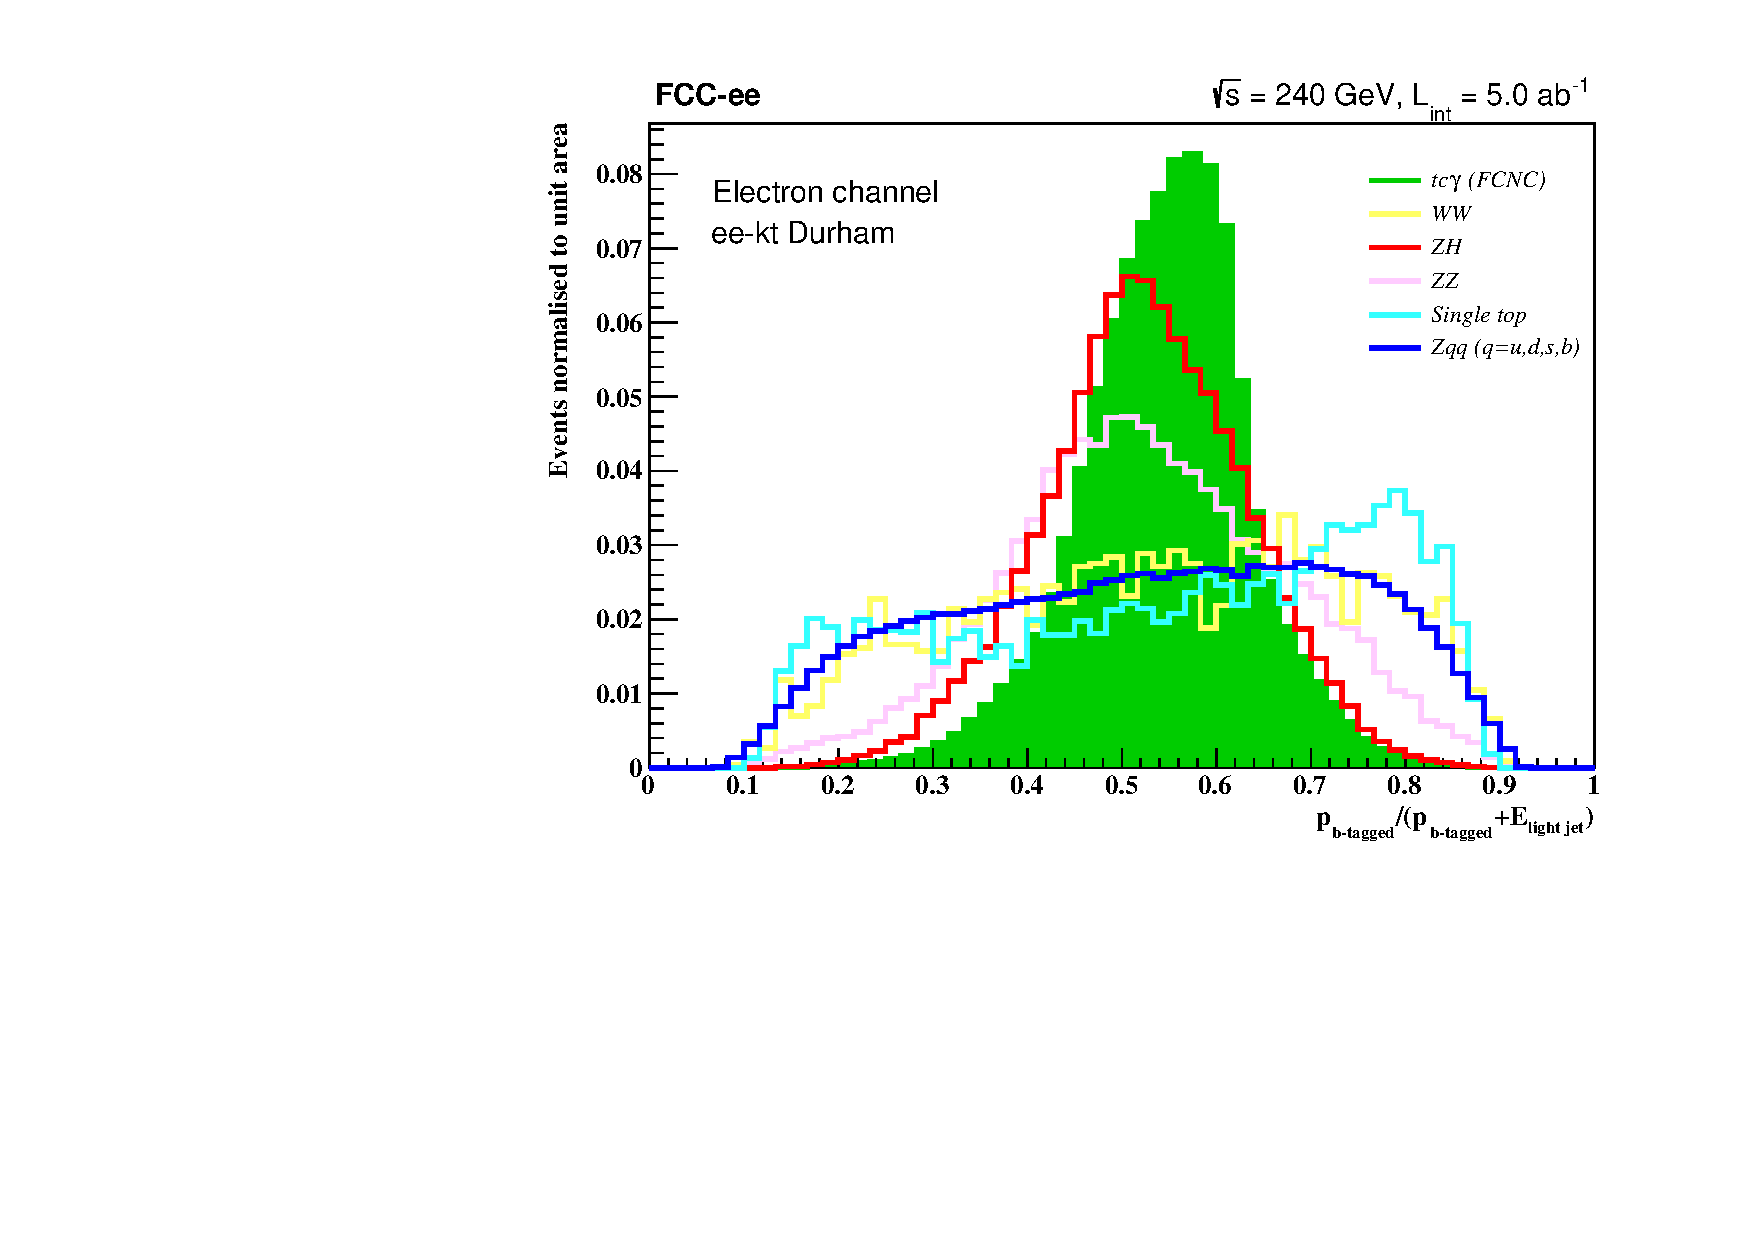
\includegraphics[width=0.45\textwidth]{240GeV-leptonic/pbpl-240GeV-leptonic.pdf}} 	
\subfloat{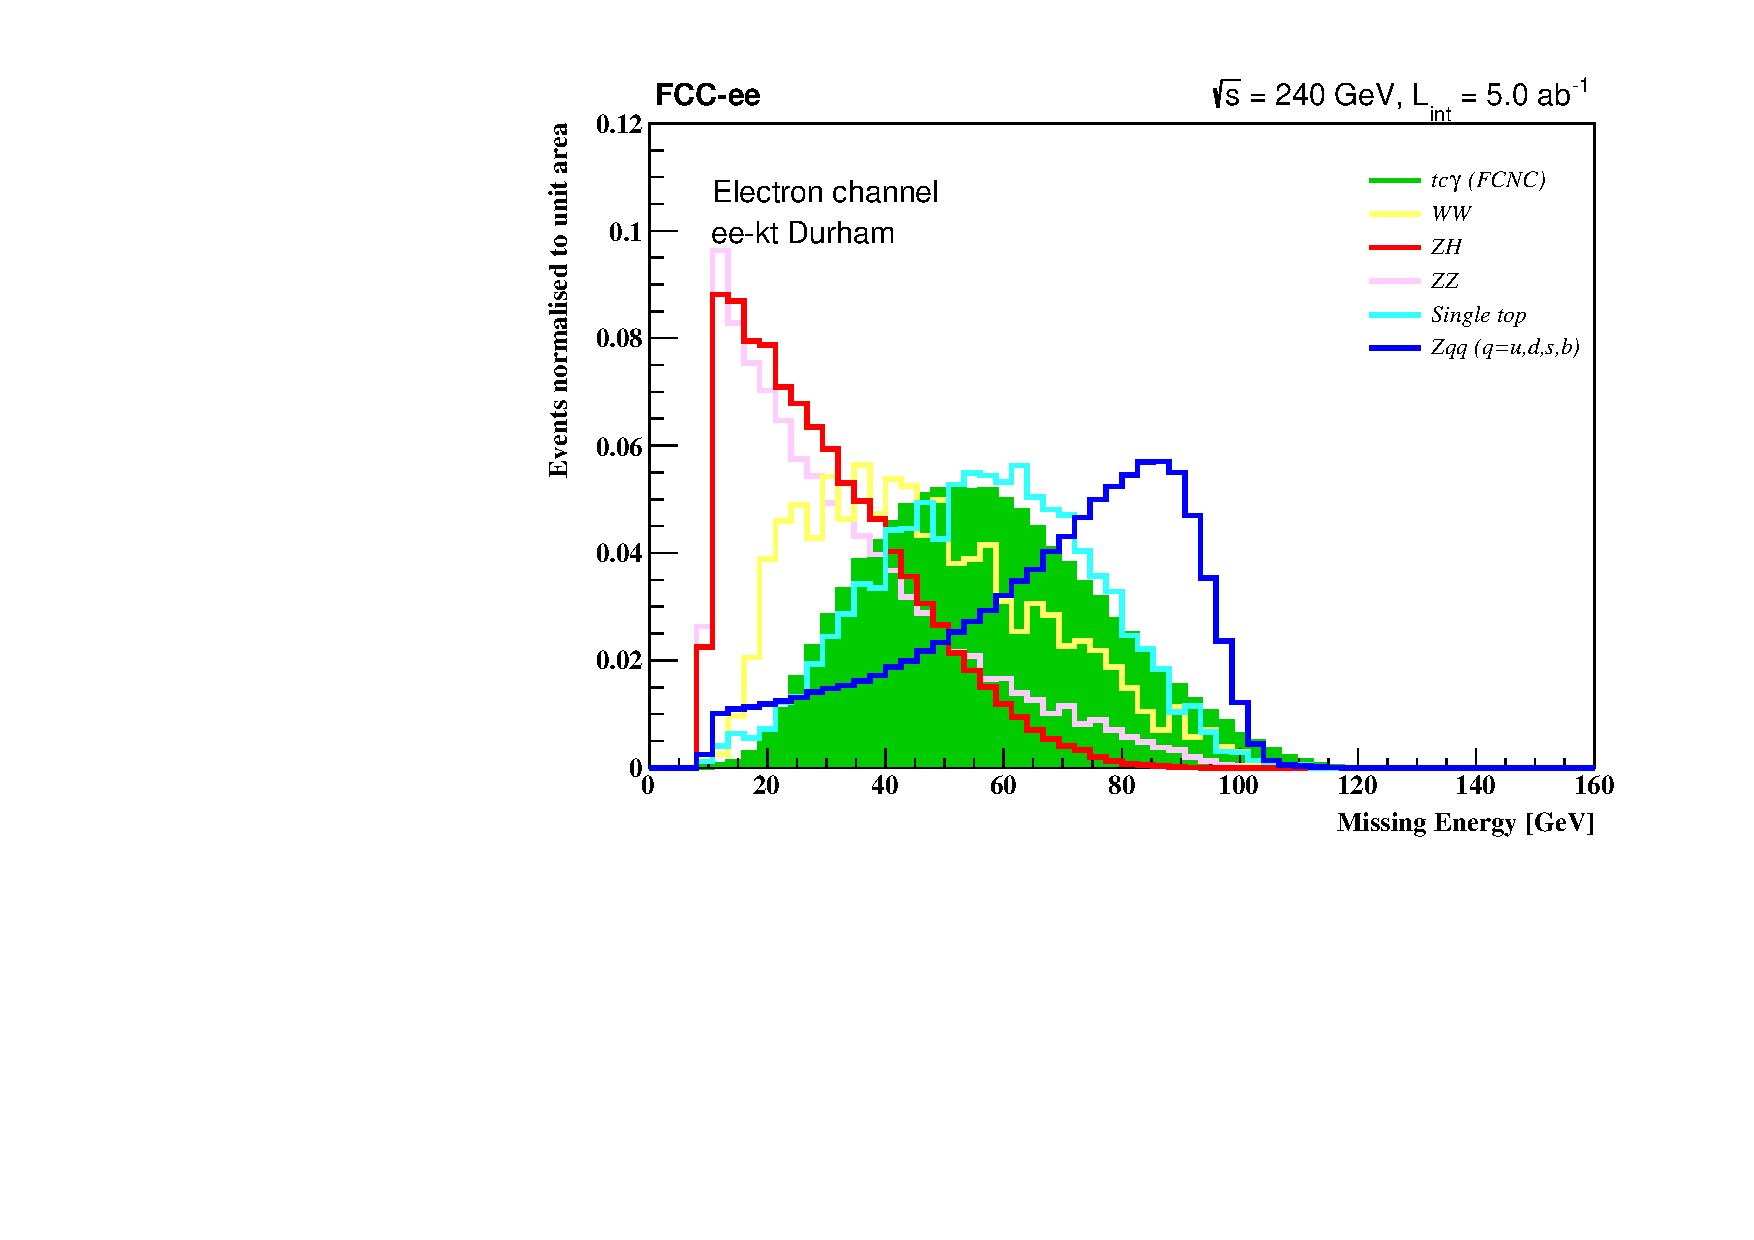
\includegraphics[width=0.45\textwidth]{240GeV-leptonic/Missing-Energy-240GeV-leptonic.pdf}}	\\
\subfloat{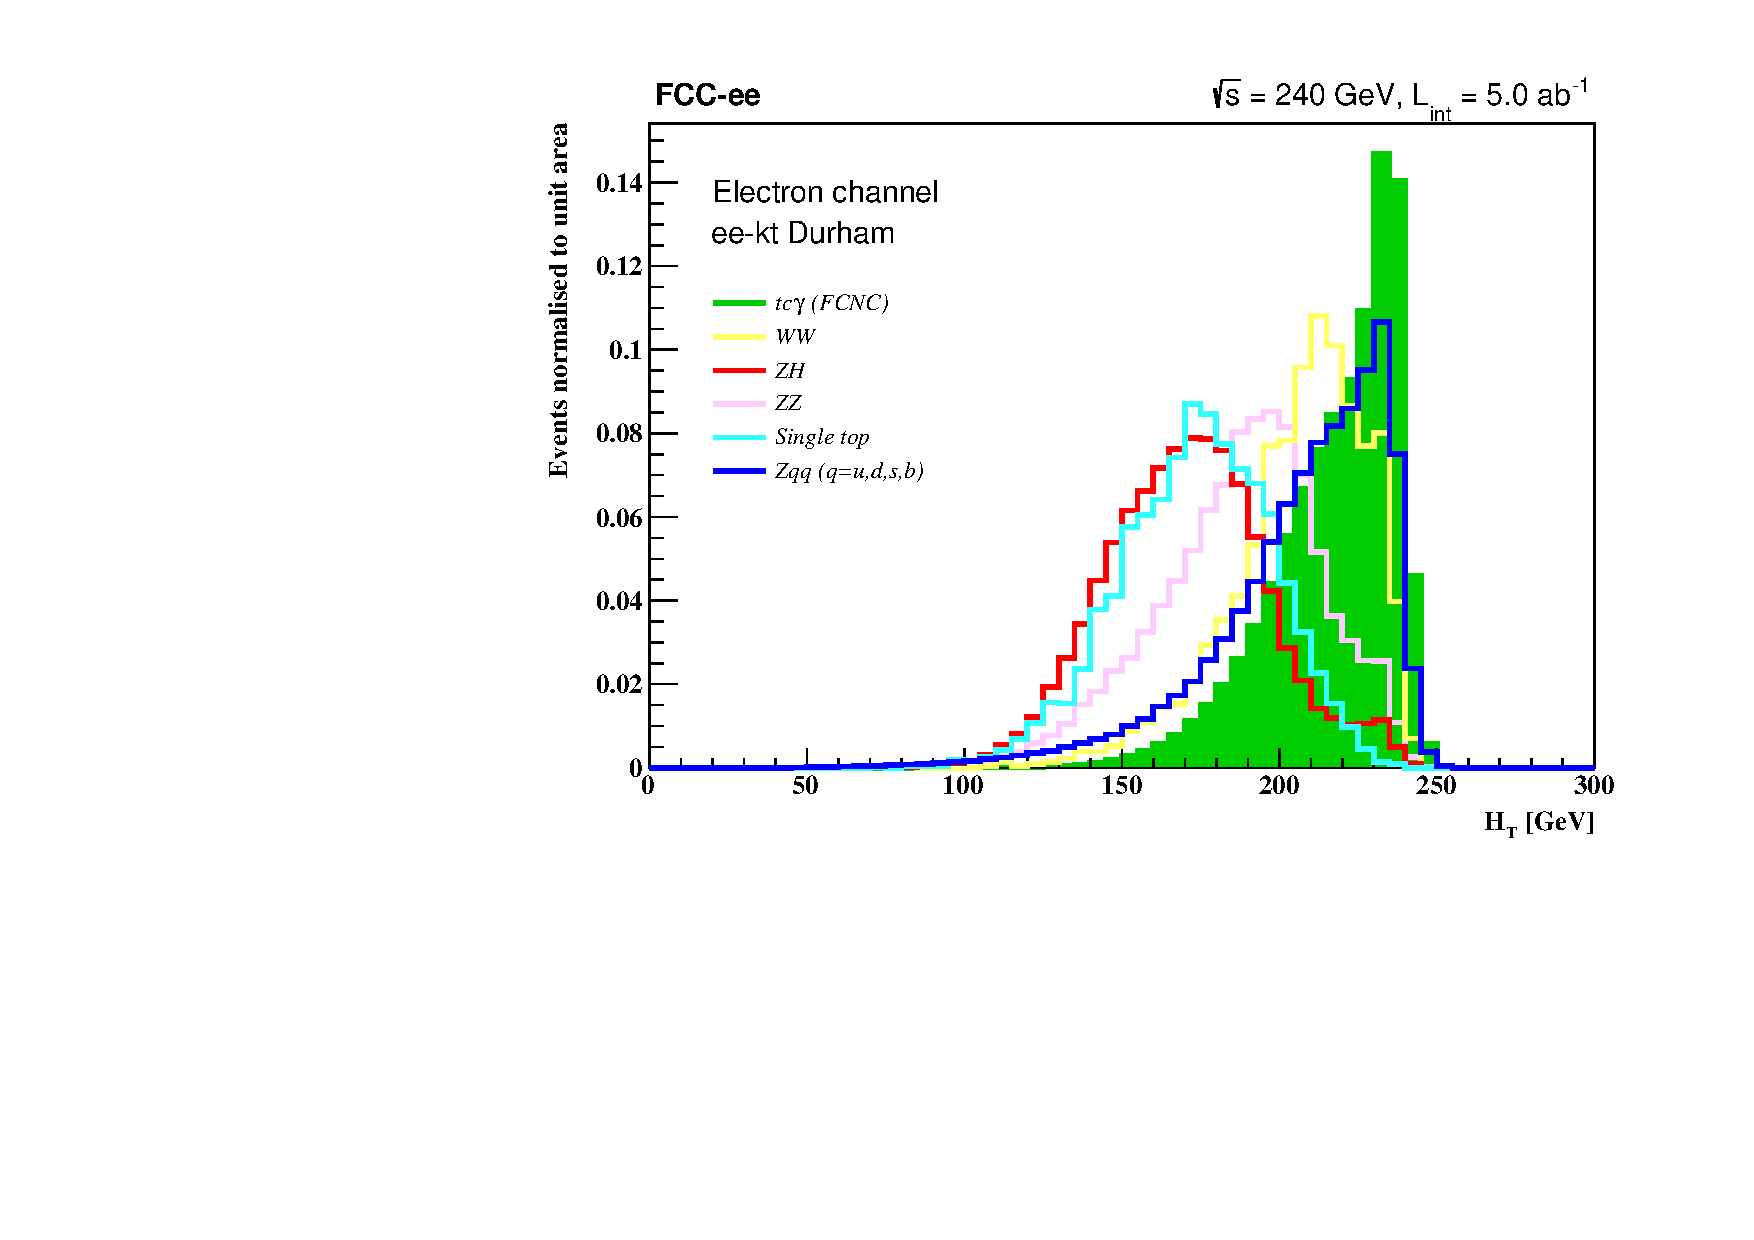
\includegraphics[width=0.45\textwidth]{240GeV-leptonic/H_T-240GeV-leptonic.pdf}} 	
\subfloat{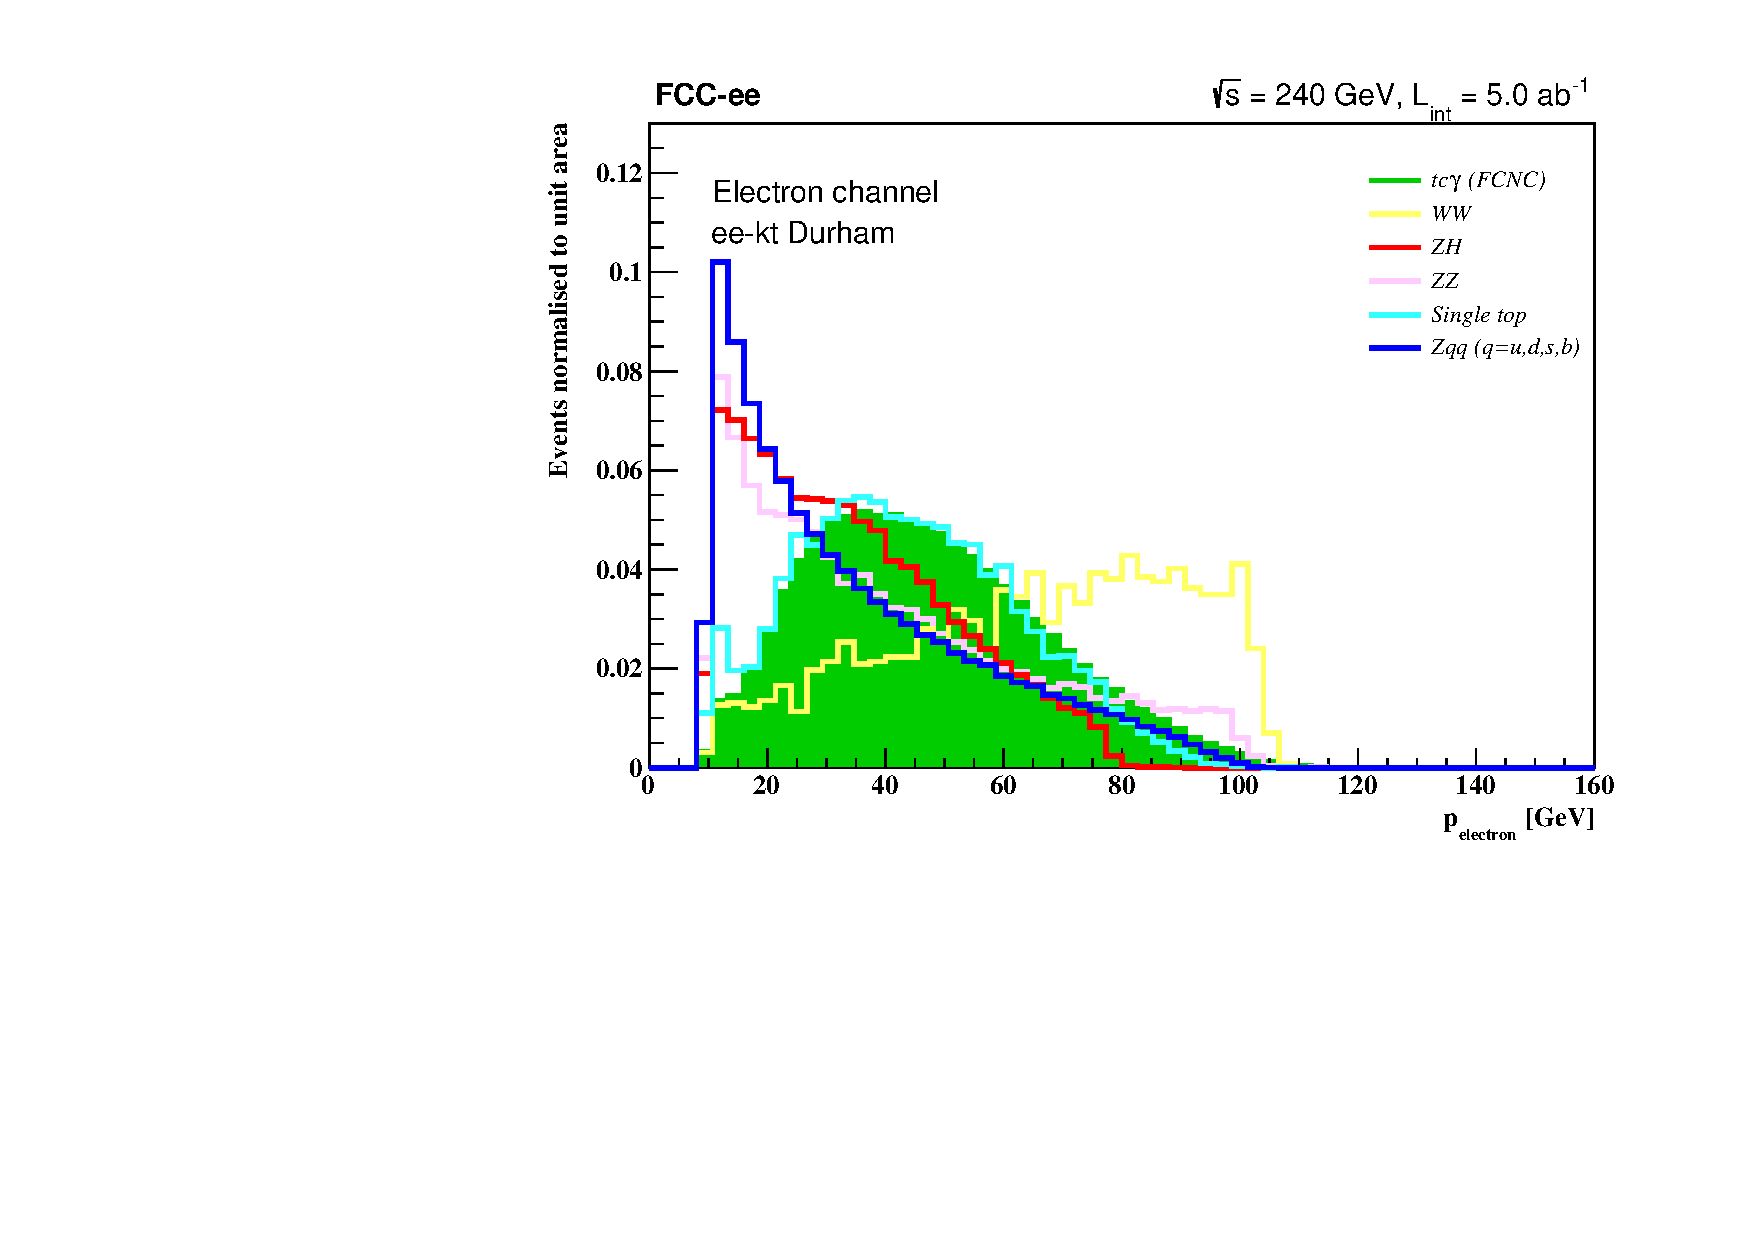
\includegraphics[width=0.45\textwidth]{240GeV-leptonic/pelectron-240GeV-leptonic.pdf}}	
%\vspace{-6cm}
\begin{center}
\caption{ \small 
The distributions for the total momentum of a $b$-tagged jet,  
the total momentum of light jets, the ratio of the total momentum of $b$-tagged jets over all jets, the 
missing energy, the scalar sum of the transverse momentum of all final state objects, and 
the total  momentum of the electron.  }
\label{variables-1}
\end{center}
\end{figure*}
%------------------------------------------------

For the center-of-mass energy of 240 GeV, the following selections are applied.

%======================
\begin{itemize}
\item Final selection cuts for the case of 240 GeV center-of-mass energy:
\begin{itemize}
\item The reconstructed top-quark mass distribution 140 GeV < $M_{\rm top}$ < 190 GeV.
\item The reconstructed W boson mass distribution  70 GeV < $M_{\rm W}$ < 90 GeV.
\item The momentum of b jet candidate  $p_{\rm bjet}$ > 40 GeV.
\item The momentum of the highest energy light jet in each event 40 GeV < $p_{light-jet}$ < 70 GeV.
\item The momentum of electron (or muon) 20 GeV < $p_{\rm electron}$ < 90 GeV.
\item The Missing Energy 30 GeV < ME < 80 GeV.
\item The angular separation between the lepton and $b$-jet,  $\Delta R (\ell, b-jet)$ < 3.5.
\item The cosine of lepton and $b$-jet, $\cos(\ell, b-jet)  < 0.85$
\item The invariant mass of di-jets, 20 GeV < $M_{(j1, j2)}$ < 150 GeV
\item The ratio of total momentum of $b$-jet to all jets, $0.35 <  \frac{p_{\rm b-jet}}{ p_{\rm b-jet}+p_{\rm light-jet}} < 0.7$.
\item The scalar sum of momentum $H_T$ > 190 GeV.
\item The total momentum of reconstructed top-quark, 40 GeV < $p^{\rm top}$ < 70 GeV
\end{itemize}
\end{itemize}
%======================
 

For the case of 365 GeV, the following selections are considered.

%======================
\begin{itemize}
\item Final selection cuts for the case of 365 GeV center-of-mass energy:
\begin{itemize}
\item The reconstructed top-quark mass distribution 140 GeV < $M_{\rm top}$ < 190 GeV.   
\item The reconstructed W boson mass distribution  70 GeV < $M_{\rm W}$ < 90 GeV.      
\item The momentum of b jet candidate  30 GeV < $p_{b-jet}$ < 140 GeV. 
\item The momentum of the highest energy light jet in each event 120 GeV < $p_{light-jet}$ < 150 GeV.
\item The momentum of electron (or muon)  20 GeV < $p_{\rm electron}$ < 100 GeV.   
\item The Missing Energy 30 GeV < ME < 120 GeV.   
\item The angular separation between the lepton and $b$-jet,  $\Delta R (\ell, b-jet)$ < 3.5.
\item The cosine of lepton and $b$-jet, $\cos(\ell, \rm b-jet) < 0.85$.
\item The invariant mass of di-jets, 100 GeV < $M_{(j1, j2)}$ < 300 GeV.
\item The ratio of total momentum of  $b$-jet to light jet, $0.2 <   \frac{p_{\rm b-jet}}{p_{\rm b-jet}+p_{\rm light-jet}} < 0.5$.
\item The scalar sum of momentum $H_T$ > 300 GeV.
\item The total momentum of reconstructed top-quark, $p^{\rm top}$ > 120 GeV.
\item The cosine of lepton and MET, $\cos(\ell, \rm MET) < 0.6$.
\end{itemize}
\end{itemize}
%======================


Taking the typical pre-selection and final-selection cuts mentioned above, 
the cross-sections of the SM backgrounds 
are presented in Table.~\ref{bkg-240} and Table.~\ref{bkg-365}
for 240 and 365 GeV, respectively. 


%======================
\begin{table*}[htbp]
\begin{center}
\begin{tabular}{l|c c c c c c  c c c c c  }  \hline
$\sqrt {s}$ = 240 GeV   ~&~ $tc\gamma$  ~&~ $tcZ$   ~&  ~  ZH     ~&  ~ WW  &  ~  ZZ ~ &~ eebb ~&~ eeqq (q=uds) ~&~ single top  \\  \hline
Cross section    ~&~  $14.327$  ~&~ $34.132$  ~&~    $201.868$        ~&~  $16438.5$   ~&~    $1358.99$  ~&~  $455.7$ ~&~  $1635.9$  ~&~  $0.010753$       \\ 
Preselection    ~&~  $3.1542$  & $7.5154$  &    $1.1953$        &  $3.75948$   &    $2.76677$  &  $19.251$ &  $0.155146$  &  $0.0003208$        \\ 
Final selection
  &  $1.3686$  & $3.2622$  &    $0.00847$        &  $0.254797$   &    $0.01127$  &  $0.1807$ &  $0.001439$  &  $3.2259\times10^{-7}$       \\   \hline  \hline
\end{tabular}
\end{center}
\caption{Cross-sections in the unit of fb for the signal scenarios 
(electron channel) and for the main SM backgrounds considered in this study 
passing pre-selection and final selection cuts at a center-of-mass energy of 240 GeV.}
\label{bkg-240}
\end{table*}
%======================






%======================
\begin{table*}[htbp]
\begin{center}
\begin{tabular}{l|c c c c  c c  c c c c c  }  \hline
$\sqrt {s}$ = 365 GeV      & $tc\gamma$  & $tcZ$   & ZH   &  WW  & ZZ & $t \bar{t}$ & eebb & single top & $tbjj$  \\  \hline
Cross section    ~&~  $25.958$  ~&~  $50.9517$    ~&~  $117.3$ ~&~    $10716.5$     ~&~  $642.8$  ~&~ $800.0$        ~&~  $615.2$  ~&~  $0.227$  ~&~ $5.98$       \\ 
Preselection    ~&~  $5.2107$  ~&~  $10.2299$    ~&~  $0.6240$ ~&~  $2.55696$     ~&~  $1.21039$  ~&~ $39.7574$    ~&~  $25.0175$  ~&~  $0.006297$  ~&~ $0.2159$       \\ 
Final selection    ~&~  $1.9599$  ~&~  $4.3406$    ~&~  $0.00410$ ~&~ $0.00857$  ~&~  $0.00809$  ~&~ $1.10752$  ~&~  $0.004332$  ~&~ $2.276\times 10^{-6}$  ~&~ $0.006947$       \\  \hline  \hline
\end{tabular}
\end{center}
\caption{Cross-sections in the unit of fb for the signal scenarios (electron channel) and 
for the main SM backgrounds considered in this study passing pre-selection 
and final selection cuts at a center-of-mass energy of 365 GeV.}
\label{bkg-365}
\end{table*}
%======================






%---------------------------------------------
\subsection{Results for the leptonic analysis}\label{leptonic-analysis}
%---------------------------------------------

 
The 95\% CL upper limits on the top FCNC decays at obtained using the CL$s$ method
at the $\sqrt {s}$ = 240 GeV are presented in Table.~\ref{limits-240}.
These limits correspond to the FCCee working at the integrated luminosity of 5 ab$^{-1}$.
The corresponding numbers for the $\sqrt {s}$ = 365 GeV and for an 
integrated luminosity of 1.5 ab$^{-1}$ are presented in Table.~\ref{limits-365} as well.




%======================
\begin{table*}[htbp]
\begin{center}
\begin{tabular}{l|c c c c }  \hline
$\sqrt {s}$ = 240 GeV  &  ~  $Br (t \to c \gamma )$       &  ~ $Br (t \to c Z)$      \\  \hline
Electron channel       &  ~  $9.60 \times 10^{-5}$        & ~ $3.53 \times 10^{-5}$       \\    
Muon channel           &  ~  $6.29 \times 10^{-5}$        & ~ $2.31 \times 10^{-5}$     \\   \hline  \hline
\end{tabular}
\end{center}
\caption{The upper limits on the top FCNC decays at $95\%$ C.L obtained using the CL$s$ method
at the $\sqrt {s}$ = 240 GeV and for an integrated luminosity of 5 ab$^{-1}$.}
\label{limits-240}
\end{table*}
%======================




%======================
\begin{table*}[htbp]
\begin{center}
\begin{tabular}{l|c c c c }  \hline
$\sqrt {s}$ = 365 GeV  &  ~  $Br (t \to c \gamma )$       &  ~ $Br (t \to c Z)$      \\  \hline
Electron channel       &  ~  $1.65 \times 10^{-4}$        & ~ $6.96 \times 10^{-5}$       \\    
Muon channel           &  ~  $1.47 \times 10^{-4}$        & ~ $6.19 \times 10^{-5}$    \\   \hline  \hline
\end{tabular}
\end{center}
\caption{Same as Table~\ref{limits-240}, but this time for the 
$\sqrt {s}$ = 365 GeV and for an integrated luminosity of 1.5 ab$^{-1}$.}
\label{limits-365}
\end{table*}
%======================







%
%%%%%%%%%%%%%%%%%%%%%%%%%%%%%%%%%%%%%%%%%%%%%%%%%%%%%%%%%%%%%%%%%%%%%%%
\subsection{Statistical combination of results in leptonic channel}\label{Combination-leptonic}
%%%%%%%%%%%%%%%%%%%%%%%%%%%%%%%%%%%%%%%%%%%%%%%%%%%%%%%%%%%%%%%%%%%%%%%
%



In Table.~\ref{limits-combination-leptonic}, the upper limits on the top FCNC 
decays at $95\%$ C.L extracted using 
the {\tt Higgs Combine Tool}~\cite{Higgs-Combination-Tool} after the statistical combination of $\sqrt {s}$ = 240 and 365 GeV are presented. 
After the statistical combination of energy and electron (muon) channels, the branching ratio of 
 $Br (t \to c \gamma ) < 1.99 \times 10^{-5}$ and $Br (t \to c Z) < 8.19 \times 10^{-6}$ 
are calculated. 

%======================
\begin{table*}[htbp]
\begin{center}
\begin{tabular}{l|c c c c }  \hline
$\sqrt {s}$ = 240 and 365 GeV  &  ~  $Br (t \to c \gamma )$       &  ~ $Br (t \to c Z)$      \\  \hline
 Energy $\&$ channel statistical combination   &  ~  $ 1.99\times 10^{-5}$        & ~ $ 8.19\times 10^{-6}$        \\   \hline  \hline
\end{tabular}
\end{center}
\caption{ The upper limits on the top FCNC decays at $95\%$ C.L obtained using 
the {\tt Higgs combination tools} after statistical  combination of $\sqrt {s}$ = 240 and 365 GeV, and electron (muon) 
channel. }
\label{limits-combination-leptonic}
\end{table*}
%======================









\clearpage





%
%%%%%%%%%%%%%%%%%%%%%%%%%%%%%%%%%%%%%%%%%%%%%%%%%%%%%%%%%%%%%%%%%%%%%%%
\subsection{Fully hadronic channel}\label{Fully-hadronic-channel}
%%%%%%%%%%%%%%%%%%%%%%%%%%%%%%%%%%%%%%%%%%%%%%%%%%%%%%%%%%%%%%%%%%%%%%%
%
In this section, we present the analysis of the FCNC $tq\gamma$ and $tqZ$ couplings in the fully hadronic decay mode of a single top-quark production process. The analysis is conducted at both 240 GeV and 365 GeV center-of-mass energies.
For this analysis, we utilize officially generated signal samples, which include: 
\begin{itemize}
\item  {\tt mgp8\_ee\_fullhad\_FCNC\_tuz\_ecm240}
\item  {\tt mgp8\_ee\_fullhad\_FCNC\_tua\_ecm240} 
\item  {\tt mgp8\_ee\_fullhad\_FCNC\_tuz\_ecm365}
\item  {\tt mgp8\_ee\_fullhad\_FCNC\_tua\_ecm365} 
\end{itemize}
For the hadronic samples, we adopt the same configurations that were utilized during the spring 2021 campaign.
To perform the jet clustering, we employ the {\tt ee-kt Durham} algorithm in conjunction with the {\tt ES} recombination scheme. Since the final state consists of four jets, we specifically focus on the exclusive mode with exactly four jets. In the case of the {\tt ee-$k_T$ Durham} algorithm, which forms the basis of our final results, we use the following configuration: {\tt JetClustering::clustering\_ee\_kt(2, 4, 1, 0)}. This configuration is readily available within the official FCCAnalysis framework.
Breaking down the arguments in {\tt JetClustering::clustering\_ee\_kt}, the first argument indicates exclusive clustering, where the event is clustered into exactly n-jets. The second argument specifies the requirement of exactly four jets in the final state. The third argument denotes the energy ordering of the jets in the final state. Lastly, the fourth argument specifies the E recombination scheme.\par
The top quark decays through the dominant mode into a b-quark and a W-boson, with the W-boson subsequently 
decaying hadronically. Therefore, the final state of the FCNC process is characterized by the presence of 4 jets, 
out of which one or two may be b-tagged jets, and the missing transverse momentum should be less than 
$20$ GeV to reduce the contribution of background events involving neutrinos.

We define three signal regions due to the varying number of required b-jets. In each of these regions, it is necessary for exactly one of the non-b-tagged jets to be classified as a light jet. All jets must have a transverse momentum of at least 20 GeV and a polar angle greater than 13 degrees. Additionally, events containing a lepton (either an electron or a muon) with a transverse momentum of at least 15 GeV are vetoed.
In signal region 1, we select events with exactly 4 jets, none of which are b-tagged. In signal region 2, we require exactly 4 jets, with one of them being b-tagged. In signal region 3, events with exactly 4 jets, with 2 of them being b-tagged, are selected.
In cases where no b-tagged jets are present, we reconstruct top quark candidates based on the signal hypothesis. The kinematics of the top quark and W-boson candidates can be reconstructed from the corresponding decay particles by minimizing the following equation:
%---------------------------------
\begin{equation}\label{xi2}
  \chi^2 = (M_W - M_{j_nj_m}^{\text{reco}})^2 + (M_{\text{top}}-M_{j_n j_m j_l}^{\text{reco}})^2,
\end{equation}
%---------------------------------
The equation represents the minimization of the chi-squared ($\chi^2$) value for each signal region, where $M_{j_nj_m}$ denotes the reconstructed mass of the W system, and $M_{j_n j_m j_l}$ represents the reconstructed mass of the bW system. The process of minimizing the $\chi^2$ value follows specific steps for each signal region.
In signal region 1, we consider the jet permutation where any non-b-tagged jet can be assigned to $j_n, j_m, j_l$. This allows us to explore all possible combinations of assigning jets to the reconstructed particles and find the permutation that yields the minimum $\chi^2$ value.
In signal region 2, the jet permutation is considered such that any non-b-tagged jet can be assigned to either $j_n$ or $j_m$, while $j_l$ must correspond to a b-tagged jet.
For signal region 3, any b-tagged jet can be assigned as $j_l$, and one of the remaining jets ($j_n$) must correspond to a non-b-tagged jet. The remaining jet ($j_m$) is then assigned accordingly.
In Equation (1), the central values of $M_W = 80.37$ GeV and $M_{\text{top}} = 172.76$ GeV are considered for the masses of the W boson and the top quark, respectively.
%For the event with more than one $b$ jet, we select the one with the higher energy 
%to reconstruct the top quark, and the one with lower energy is used to reconstruct 
%the W boson.
%Among the light jets, the one with the lower energy is considered to 
%reconstruct the W boson. 
We use the same backgrounds listed in the previous section.   

Based on the aforementioned selection, we performed the reconstruction 
of the W mass and top-quark mass distributions. These distributions are 
depicted in Figures \ref{W-top-mass-full-240GeV} and \ref{W-top-mass-full-365GeV}. 
Specifically, the distributions showcase the $tc\gamma$ signal alongside the primary 
backgrounds at center-of-mass energies of $\sqrt{s} = 240$ GeV and $\sqrt{s} = 365$ GeV, respectively.


%------------------------------------------------
\begin{figure*}[htb]
\vspace{0.50cm}
\centering
\subfloat{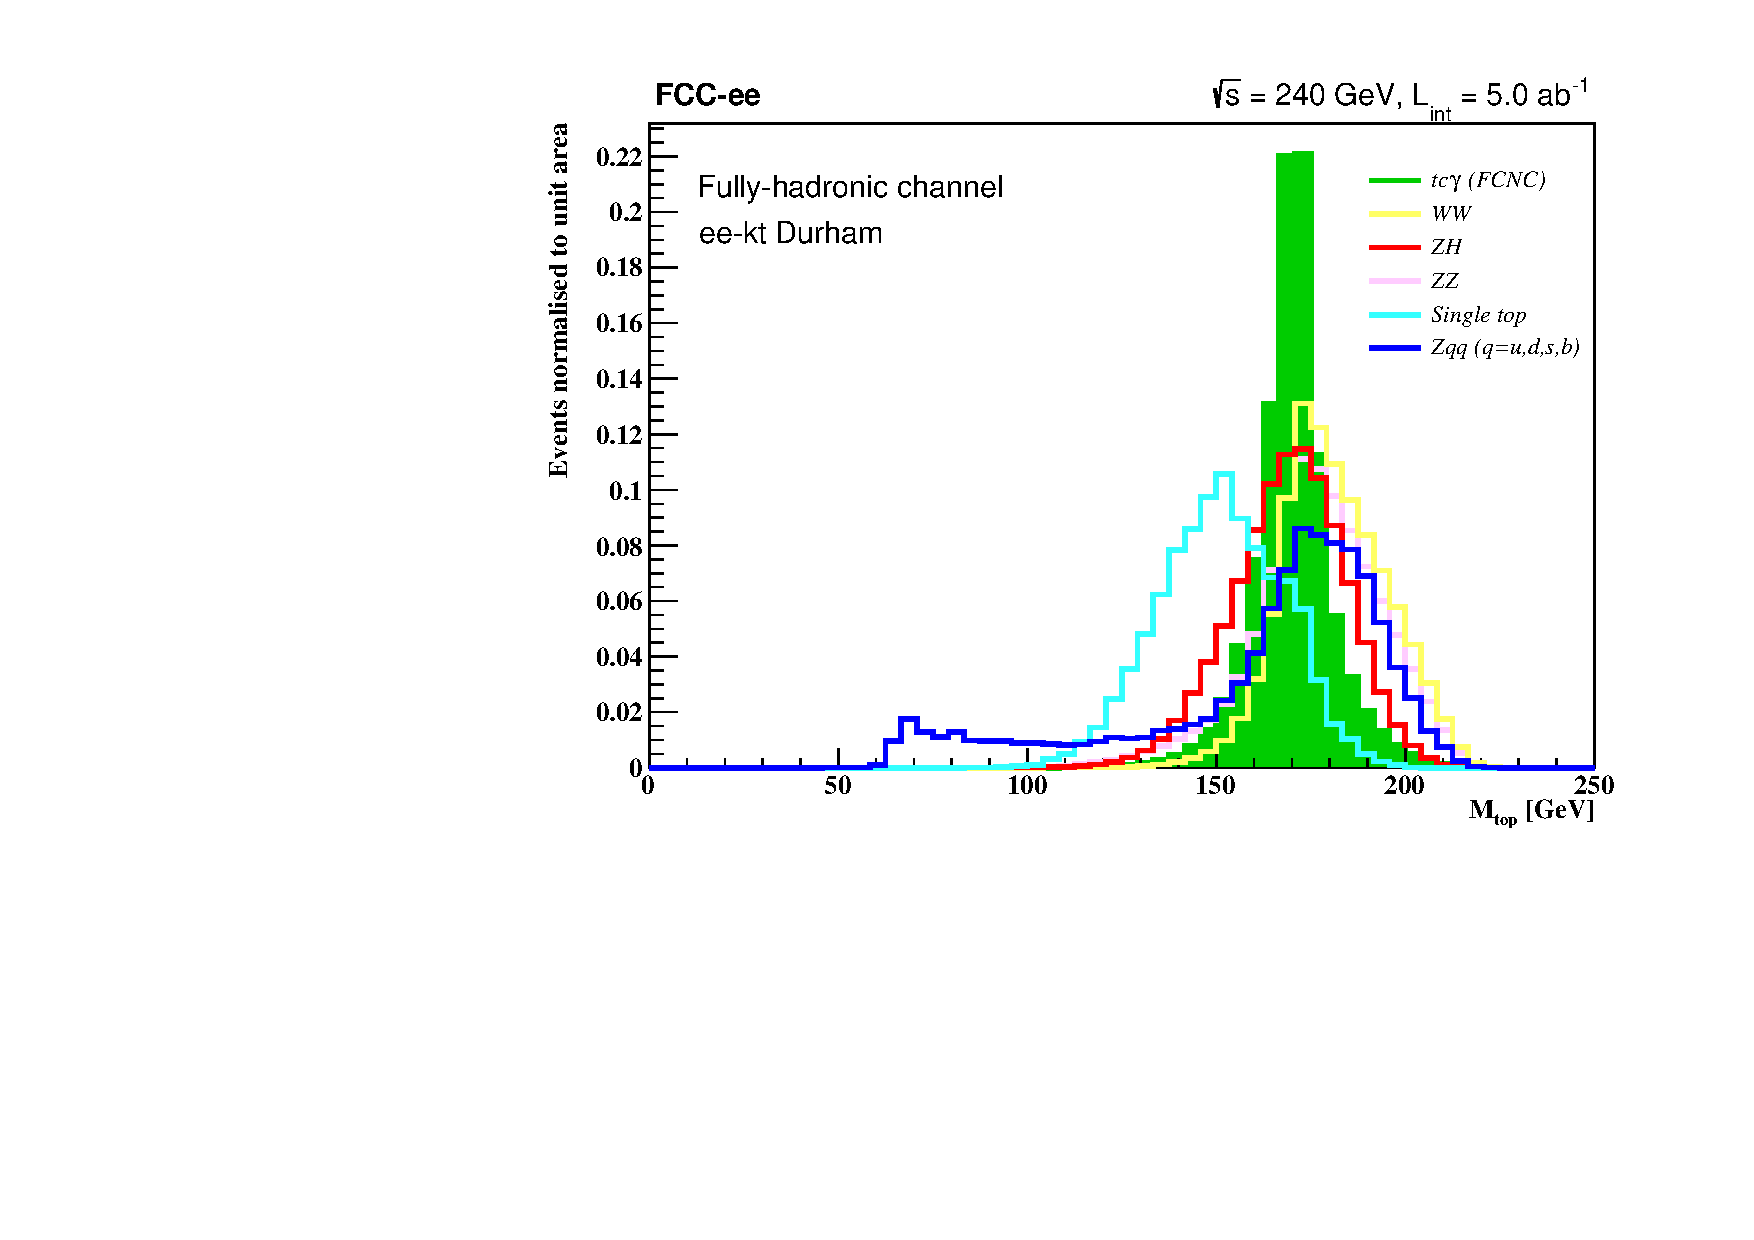
\includegraphics[width=0.45\textwidth]{240GeV-fullhadonic/topmass-full-240GeV.pdf}} 	
\subfloat{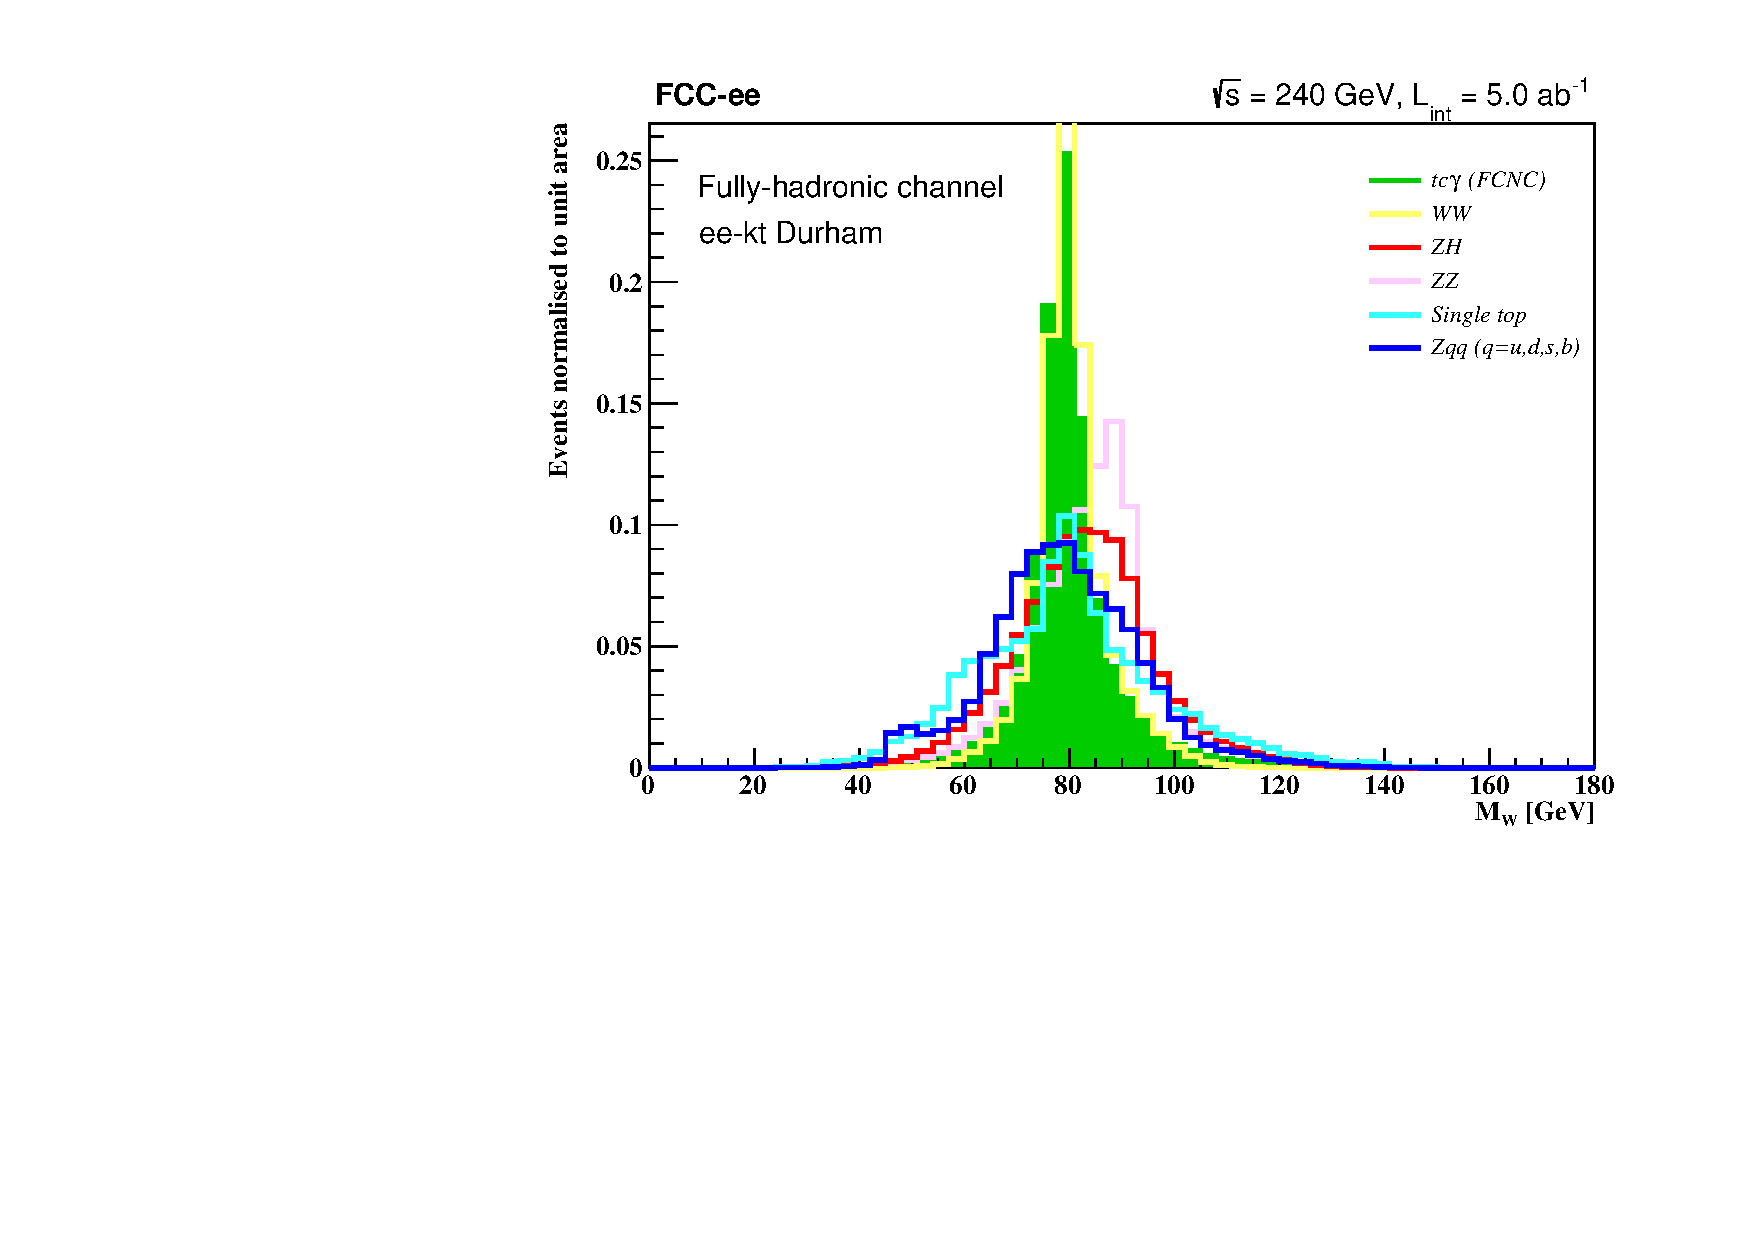
\includegraphics[width=0.45\textwidth]{240GeV-fullhadonic/Wmass-full-240GeV.pdf}}	
%\vspace{-6cm}
\begin{center}
\caption{ \small 
The mass distribution of the reconstructed top quark 
and the W boson for $tc \gamma$ signal in the presence of main backgrounds  
for the full-hadronic analysis. The distributions are shown for the $\sqrt{s}= 240$ GeV. }
\label{W-top-mass-full-240GeV}
\end{center}
\end{figure*}
%------------------------------------------------



%------------------------------------------------
\begin{figure*}[htb]
\vspace{0.50cm}
\centering
\subfloat{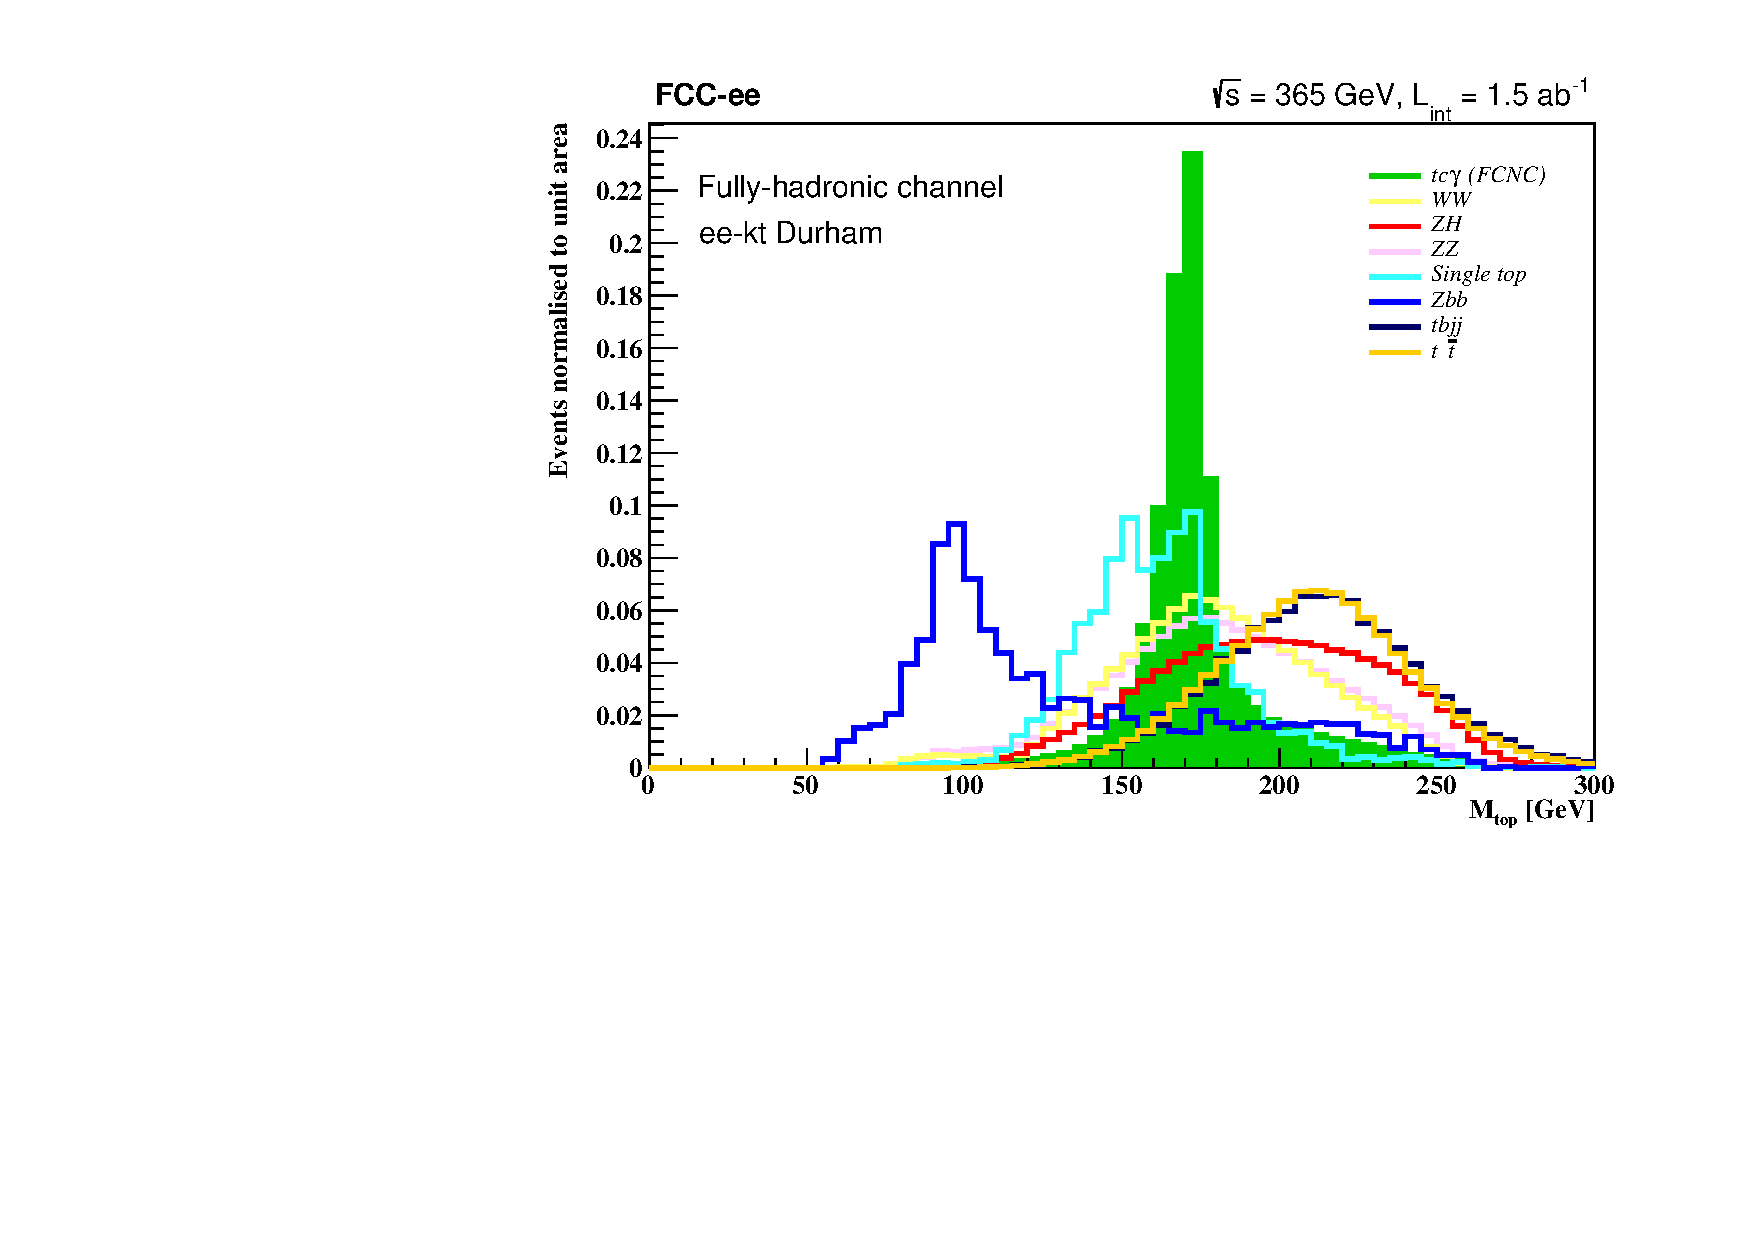
\includegraphics[width=0.45\textwidth]{365GeV-fullhadronic/topmass-full-365GeV.pdf}} 	
\subfloat{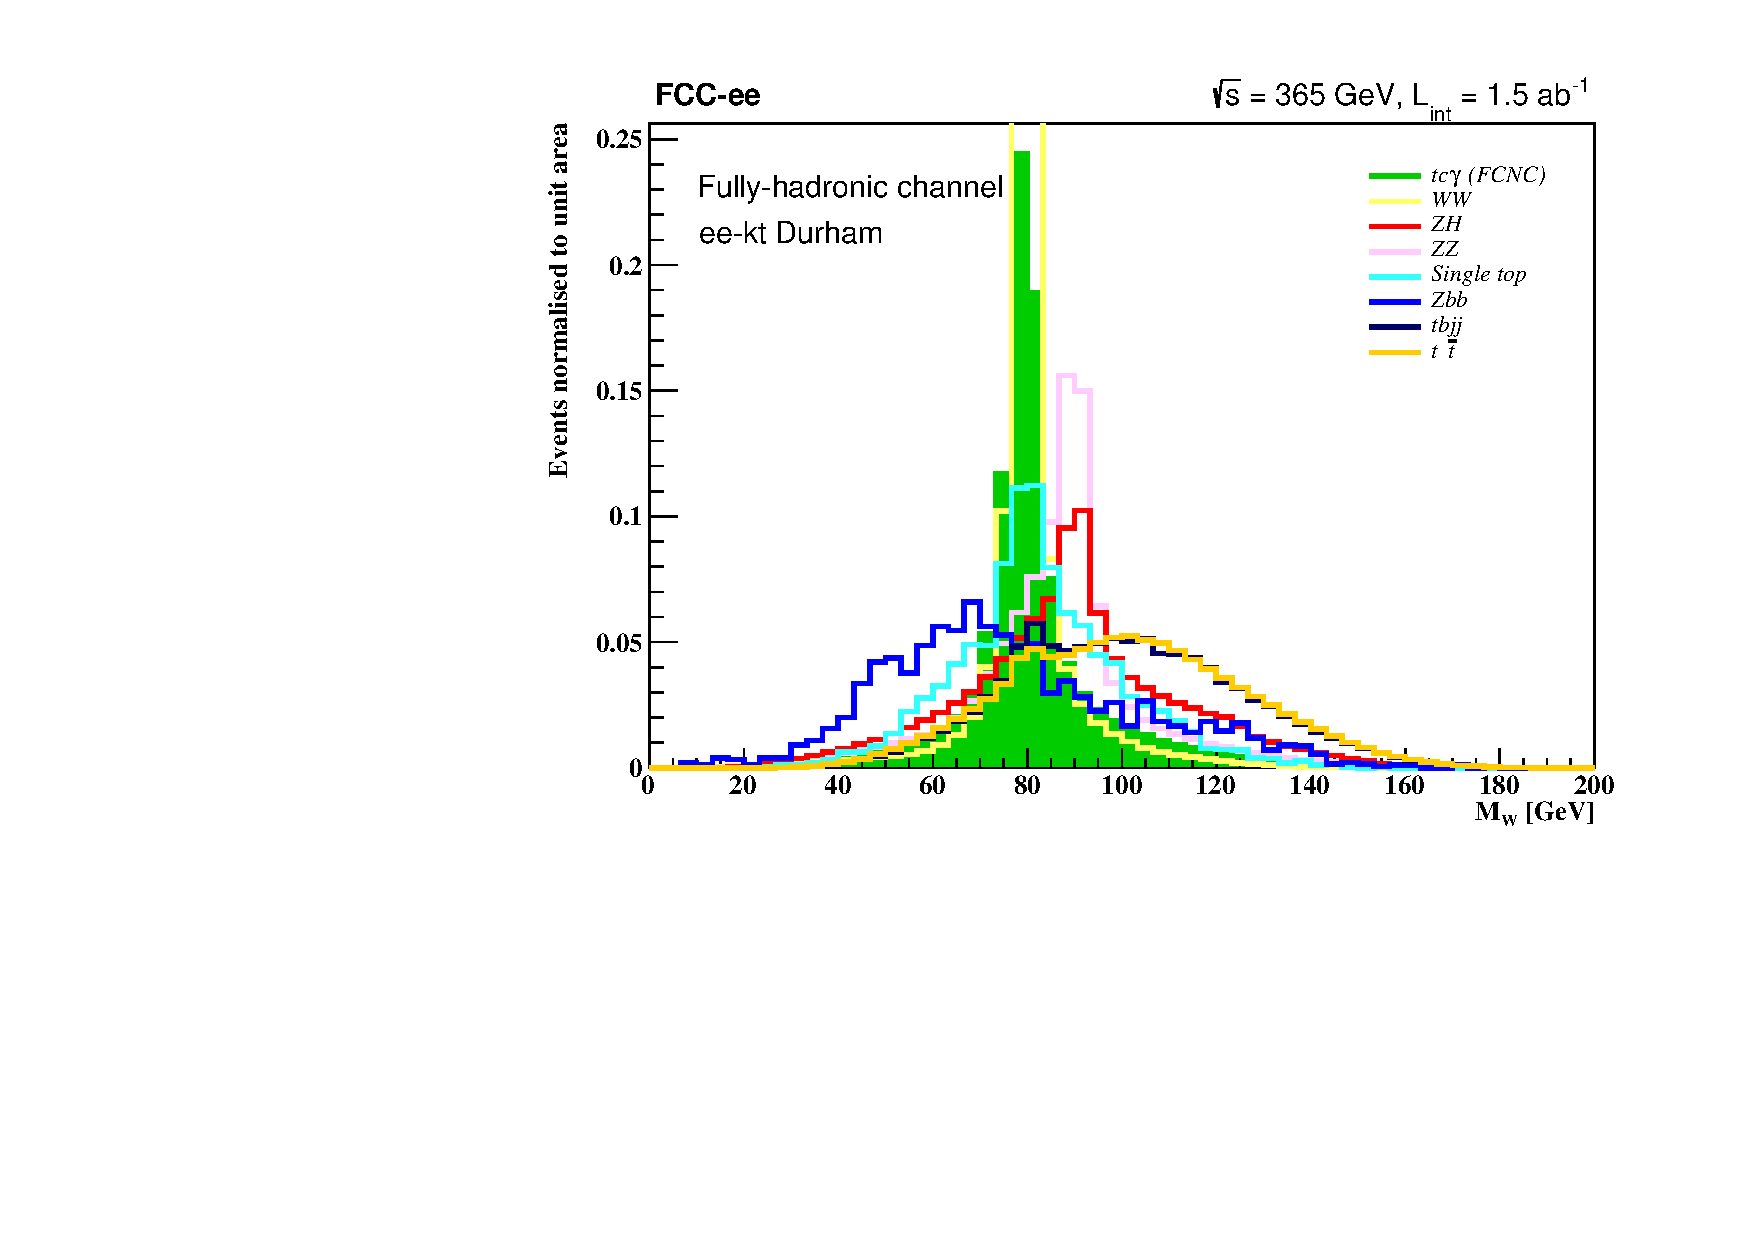
\includegraphics[width=0.45\textwidth]{365GeV-fullhadronic/Wmass-full-365GeV.pdf}}	
%\vspace{-6cm}
\begin{center}
\caption{ \small 
The mass distribution of the reconstructed top quark 
and the W boson for $tc \gamma$ signal in the presence of main backgrounds  
for the full-hadronic analysis. The distributions are shown for the $\sqrt{s}= 365$ GeV. }
\label{W-top-mass-full-365GeV}
\end{center}
\end{figure*}
%------------------------------------------------

In addition to the W mass and top-quark mass distributions, we have utilized several other distributions that 
exhibit significant discrimination power for separating the signal from backgrounds. 
These distributions are presented in Fig~\ref{full-240GeV-1}, \ref{full-240GeV-2}, and \ref{full-240GeV-3}.  
These include the total momentum of the b-tagged jet, the light jet,  the scalar sum of  
the transverse momentum of all jets in the final state, and the total momentum of the reconstructed top quark. 
In order to better discriminate signals from the background, we also examine the missing energy, 
and we define two new distributions as a ratio of the total momentum of the light jet to the b-tagged jet.
We also use the ratio of the absolute value of momentum difference between the light jet and the b-tagged jets over 
the total momentum of $b$-tagged jets.
During our fully-hadronic analysis, we have identified that the main contribution to the background arises from WW processes. To effectively suppress this background, we utilize the reconstructed mass of the second W boson, which is present in the background but not in the signal. This mass is reconstructed using two jets that are not involved in the W boson reconstruction for the signal.
In addition, we investigate the angular separations between the jets involved in the fully hadronic analysis, including both the b-tagged and light jets. Analyzing these angular separations helps enhance the discrimination between the signal and background.
The corresponding distributions for these angular separations can be found in Figure~\ref{full-240GeV-3}.

%------------------------------------------------
\begin{figure*}[htb]
\vspace{0.50cm}
\centering
\subfloat{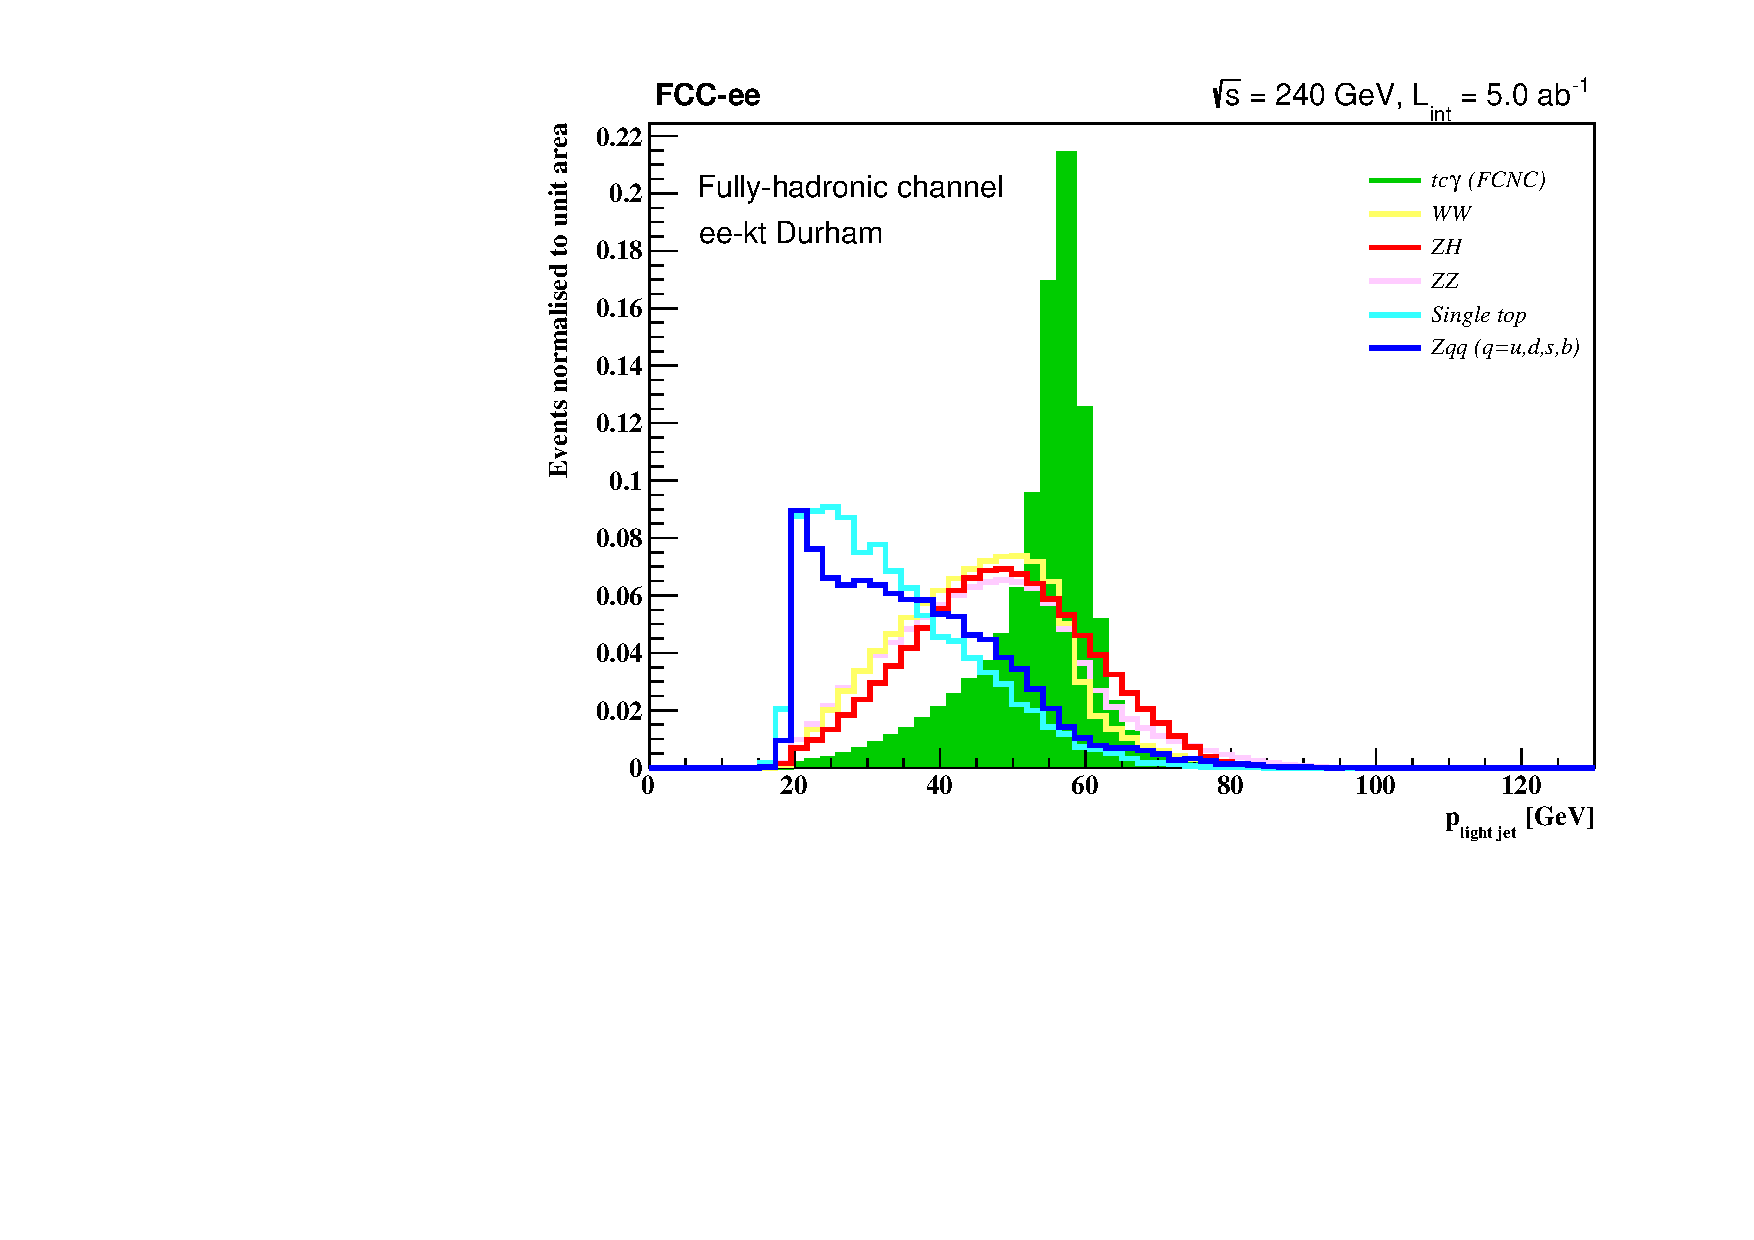
\includegraphics[width=0.45\textwidth]{240GeV-fullhadonic/plightjet-full-240GeV.pdf}} 	
\subfloat{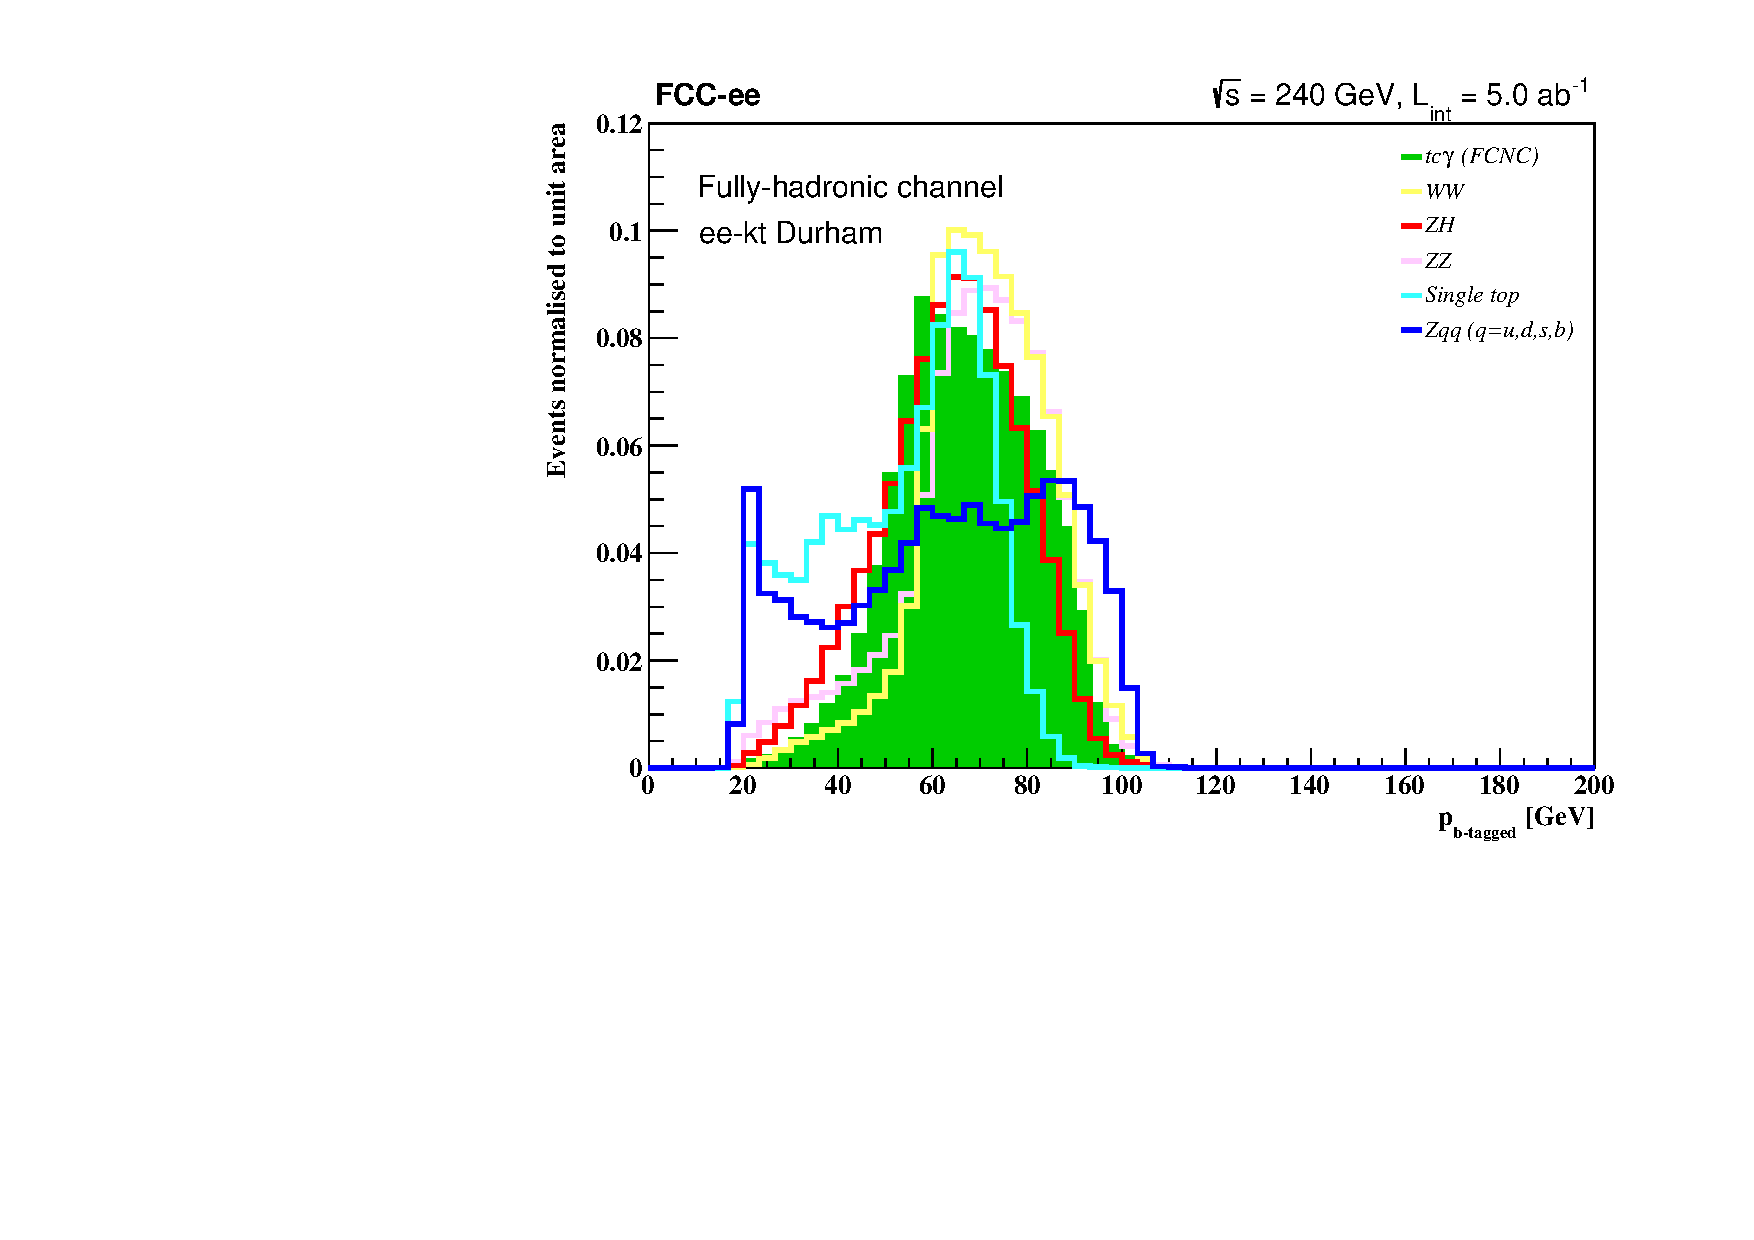
\includegraphics[width=0.45\textwidth]{240GeV-fullhadonic/pbjet-full-240GeV.pdf}} \\	
\subfloat{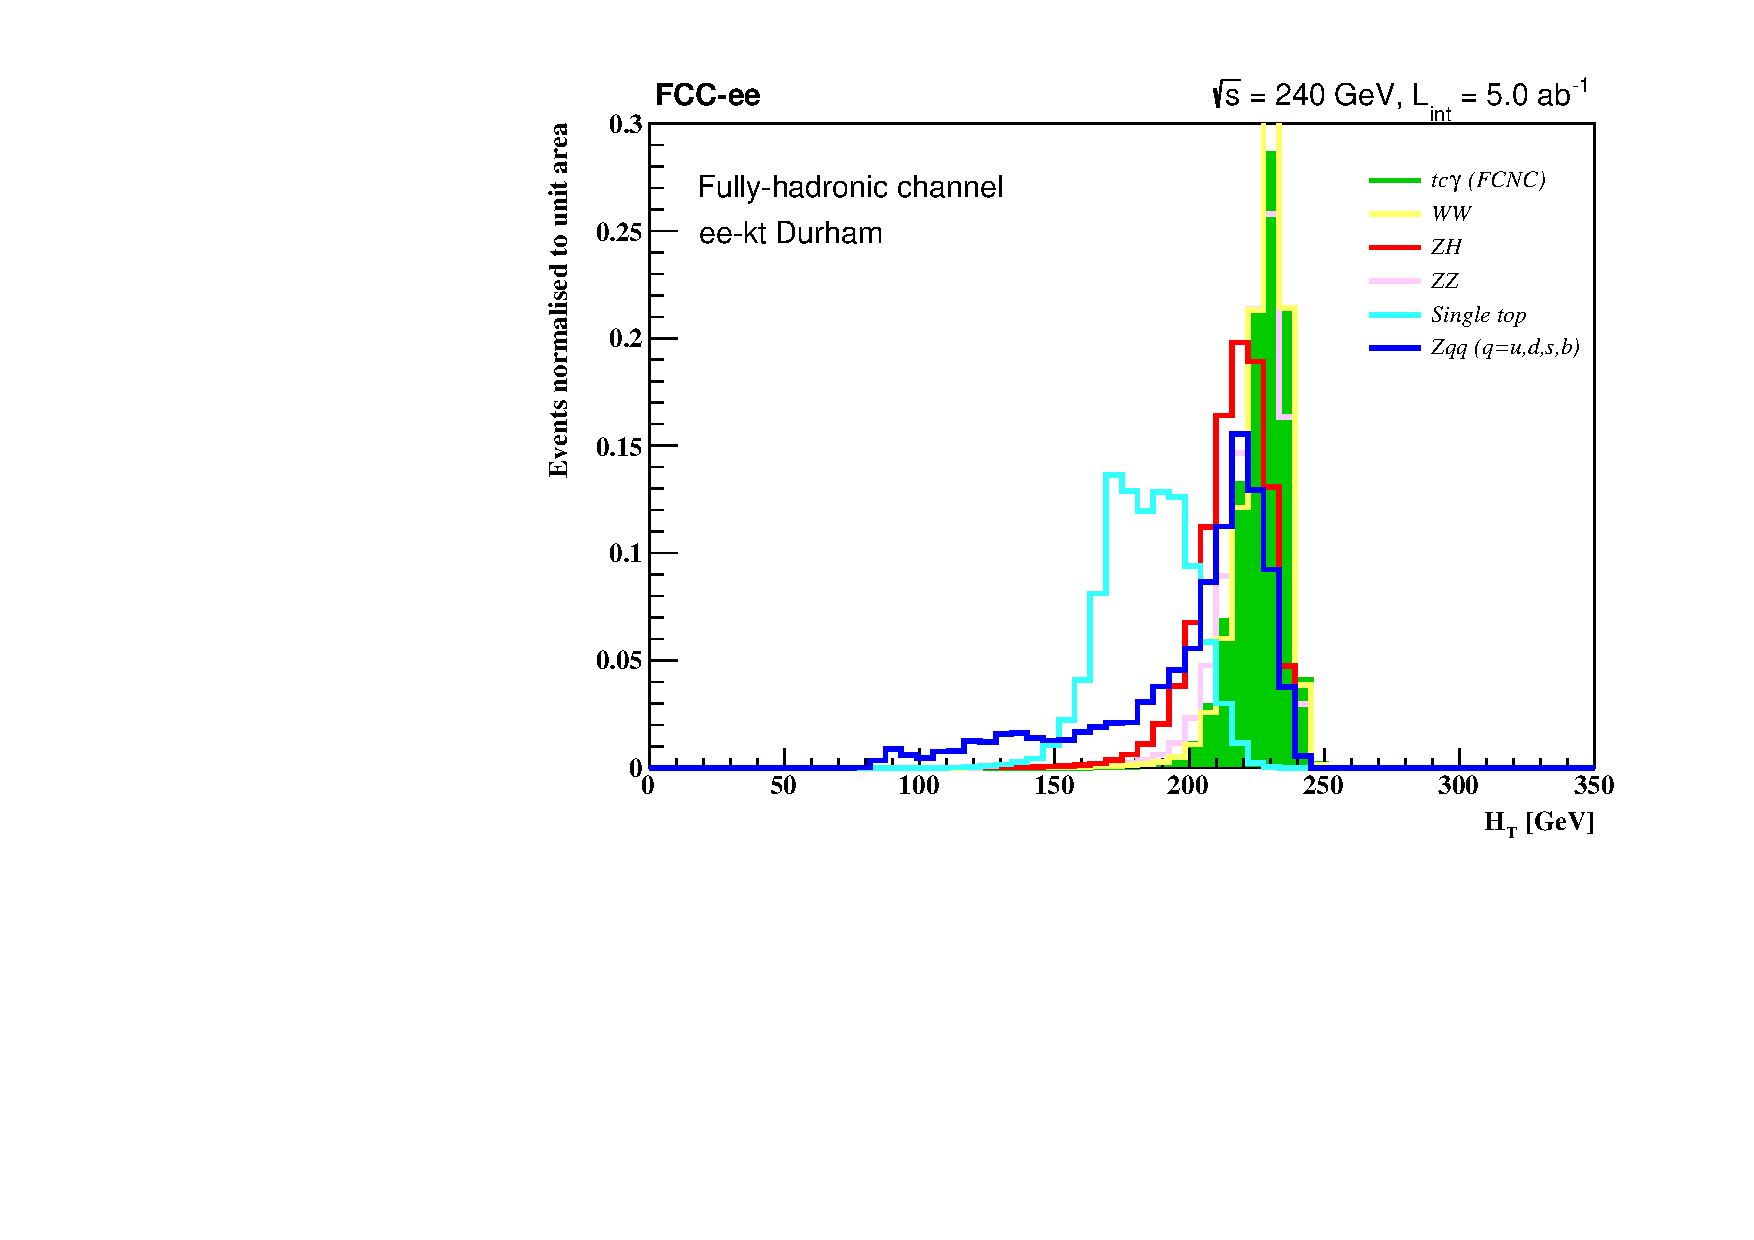
\includegraphics[width=0.45\textwidth]{240GeV-fullhadonic/H_T-full-240GeV.pdf}} 	
\subfloat{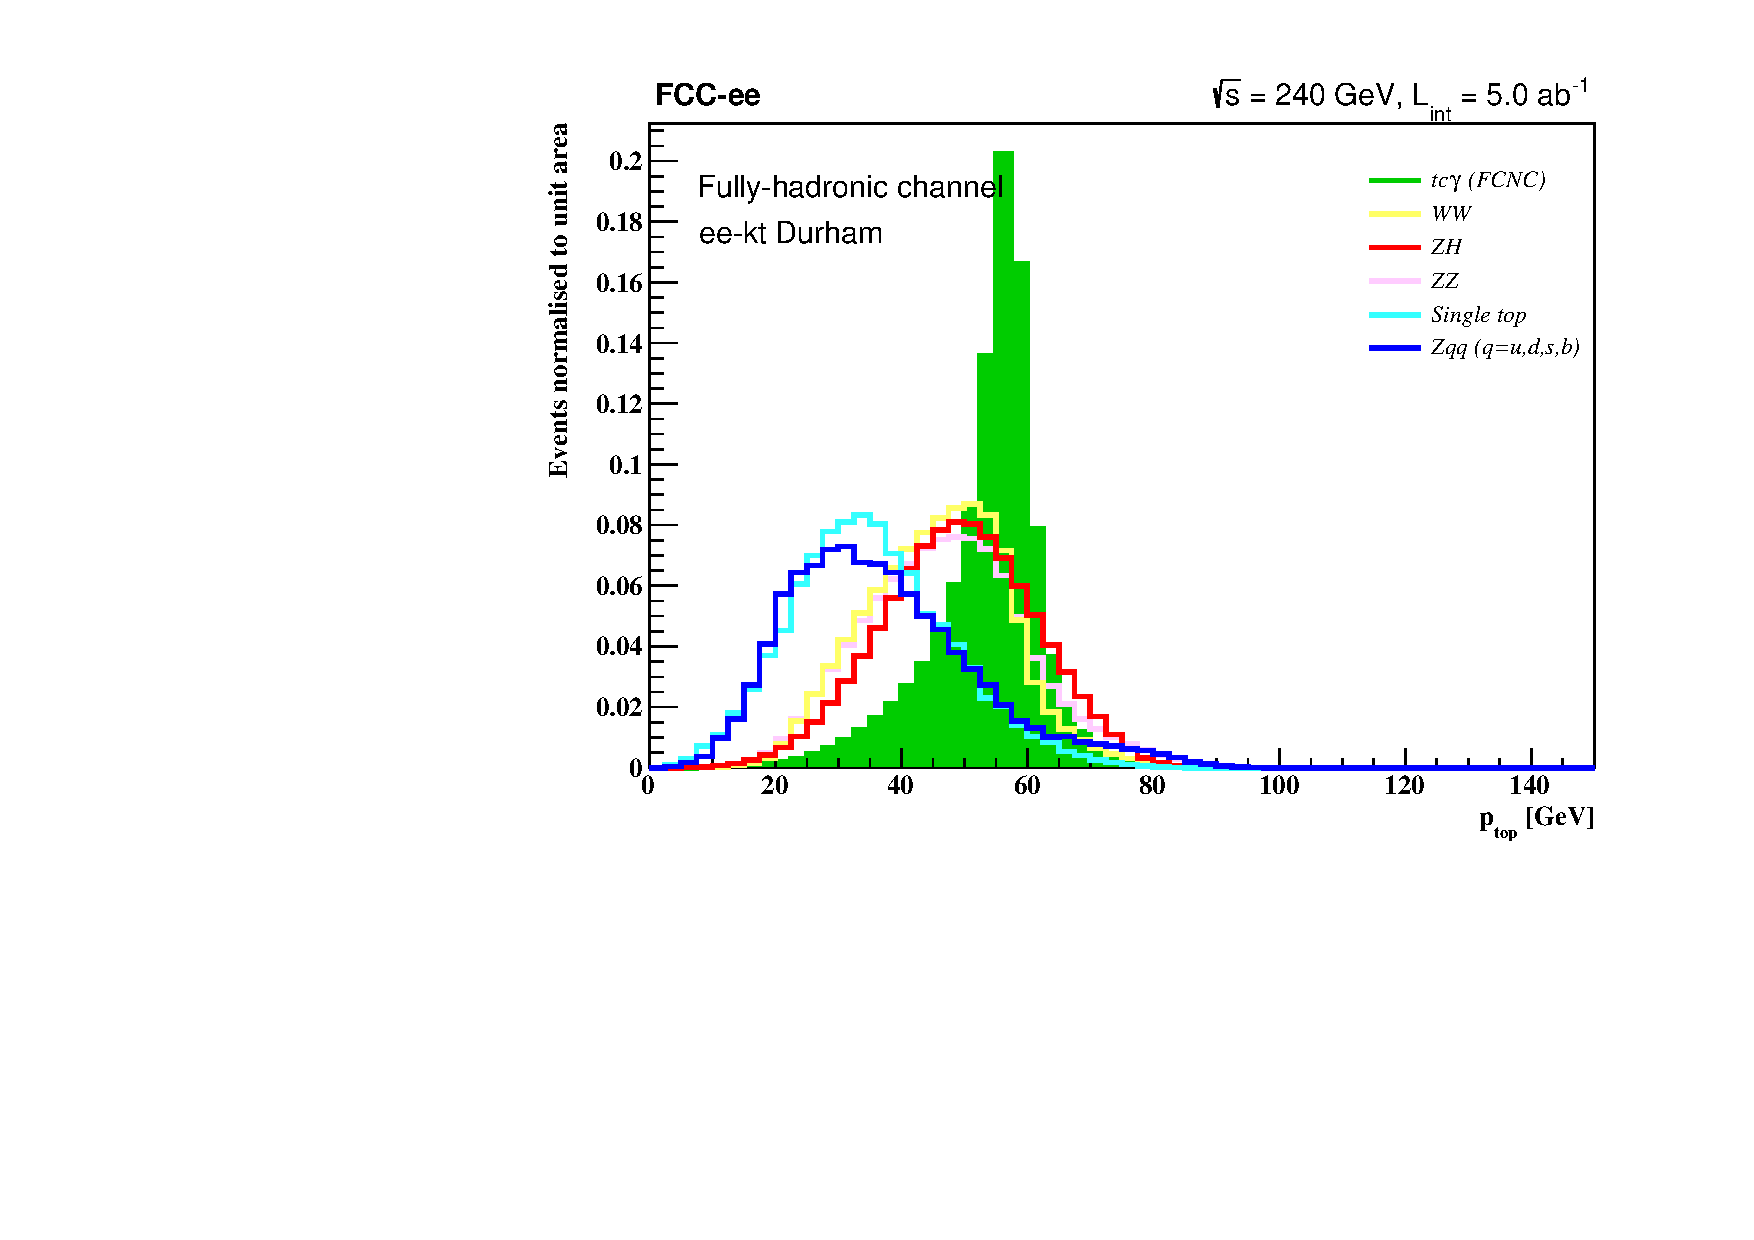
\includegraphics[width=0.45\textwidth]{240GeV-fullhadonic/ptop-full-240GeV.pdf}}	
%\vspace{-6cm}
\begin{center}
\caption{ \small 
The total momentum of the b-tagged jets, the light jets,  the scalar sum of 
the transverse momentum of all jets in the final state, and the total momentum 
of the reconstructed top quark  for the $\sqrt{s}= 240$ GeV. }
\label{full-240GeV-1}
\end{center}
\end{figure*}
%------------------------------------------------







%------------------------------------------------
\begin{figure*}[htb]
\vspace{0.50cm}
\centering
\subfloat{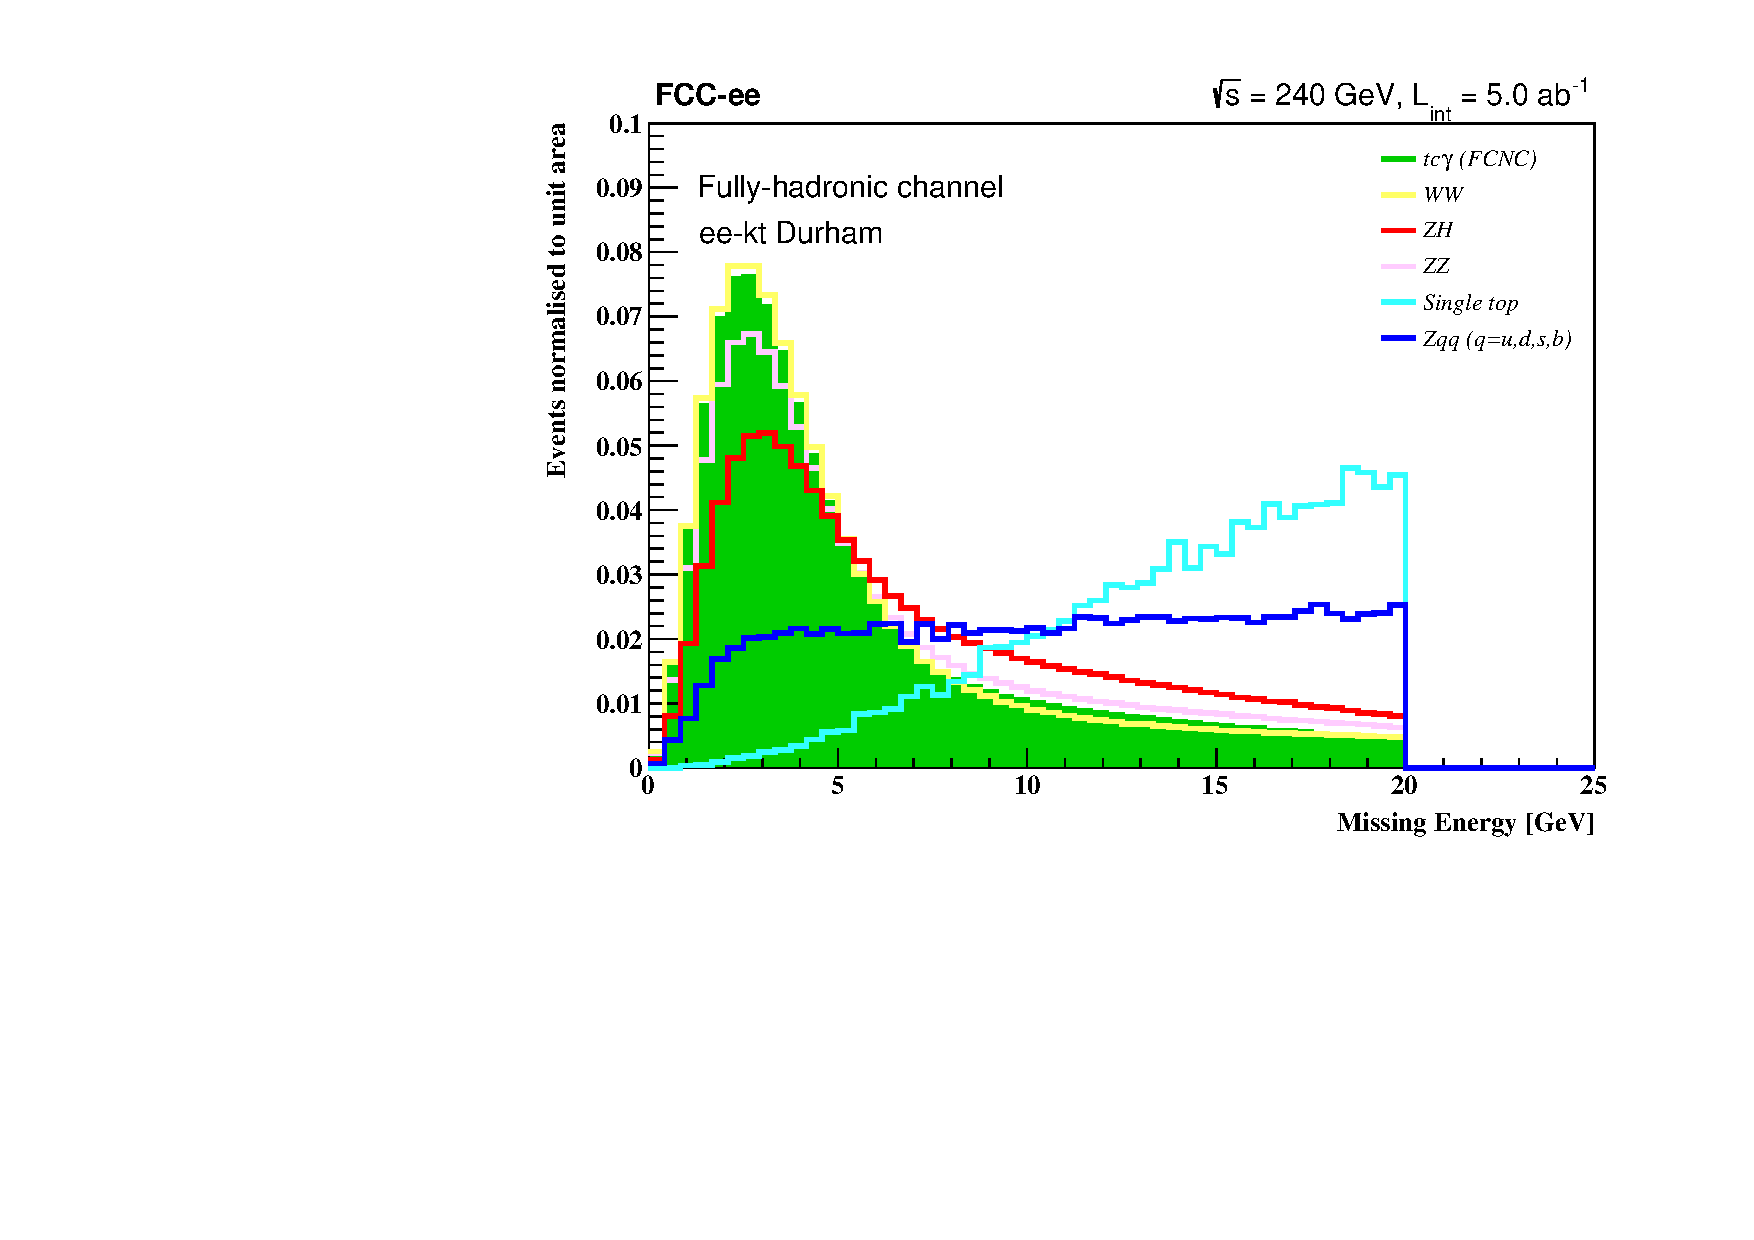
\includegraphics[width=0.45\textwidth]{240GeV-fullhadonic/Missing-Energy-full-240GeV.pdf}}	
\subfloat{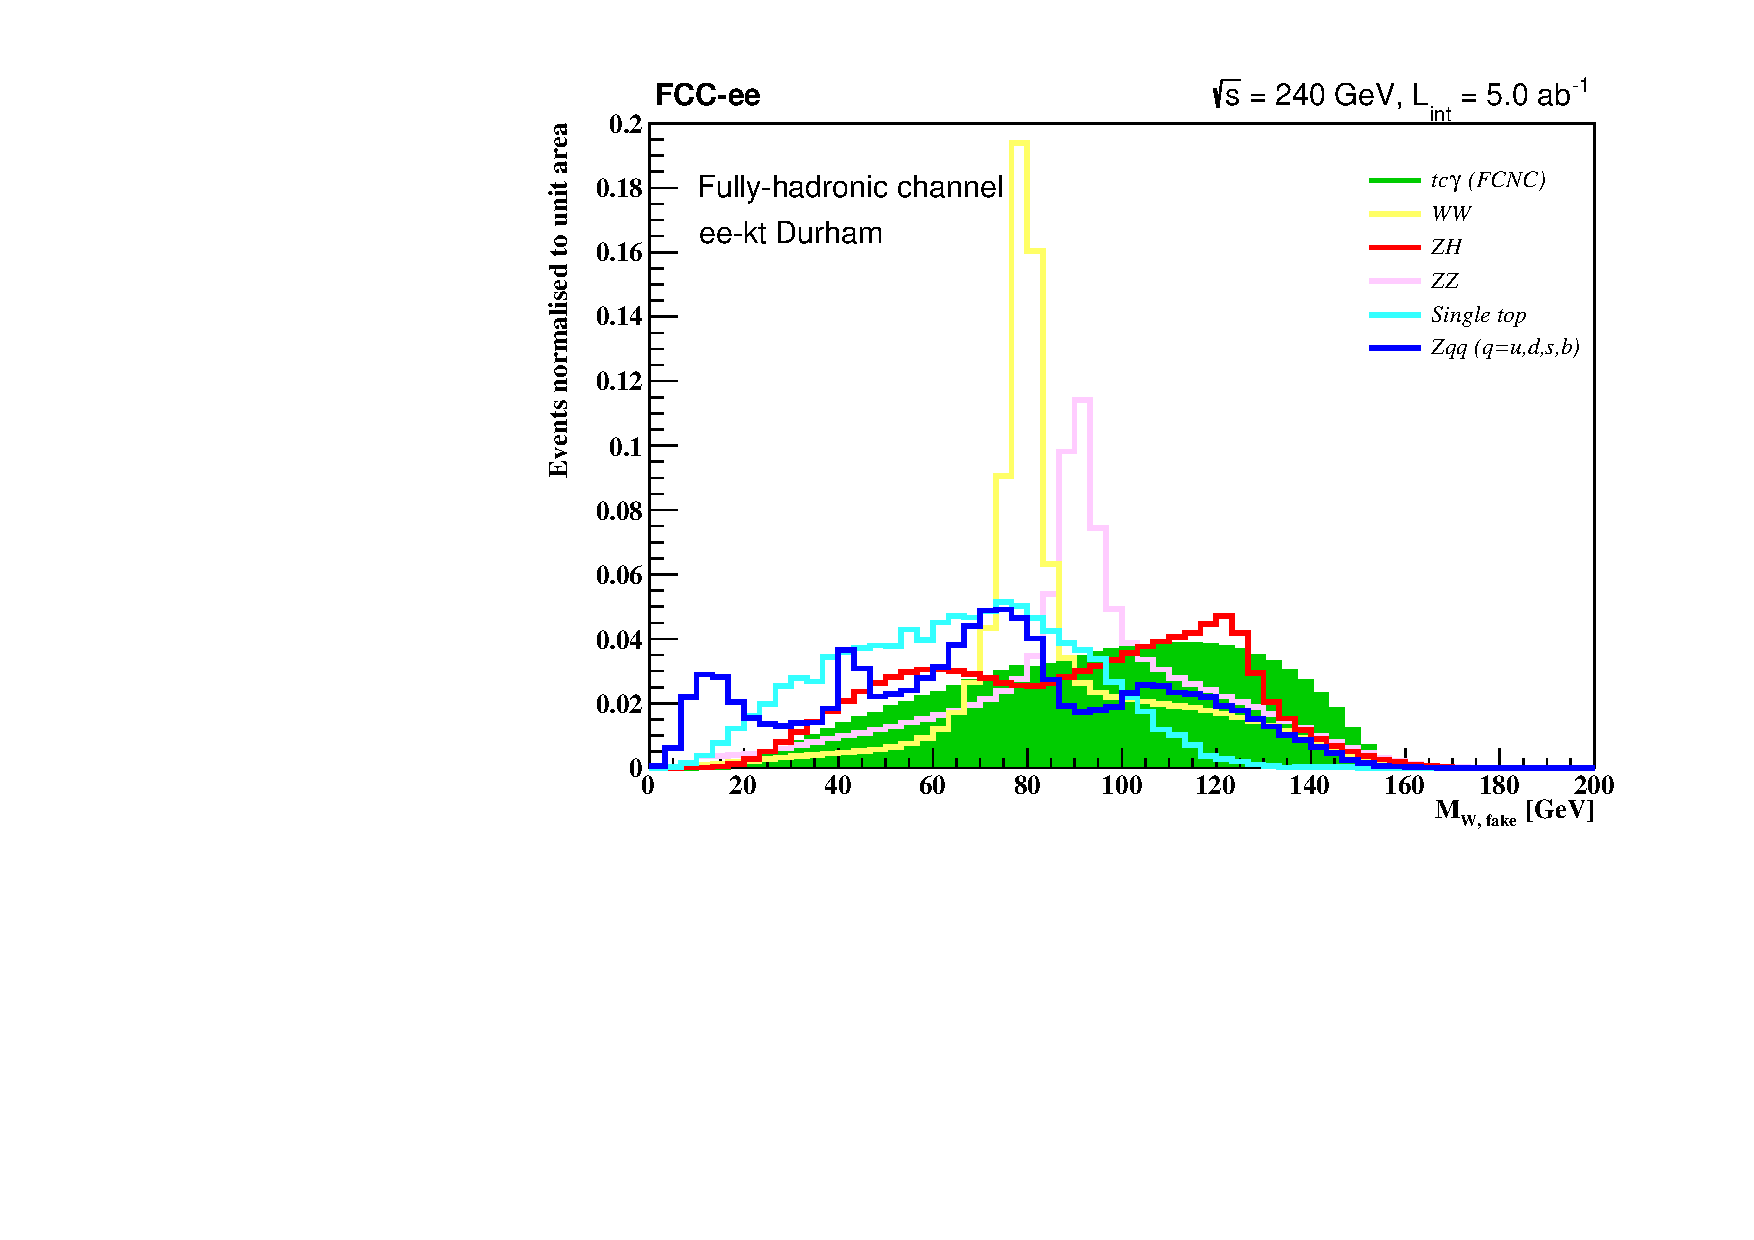
\includegraphics[width=0.45\textwidth]{240GeV-fullhadonic/FakeWmass-full-240GeV.pdf}}	 \\
\subfloat{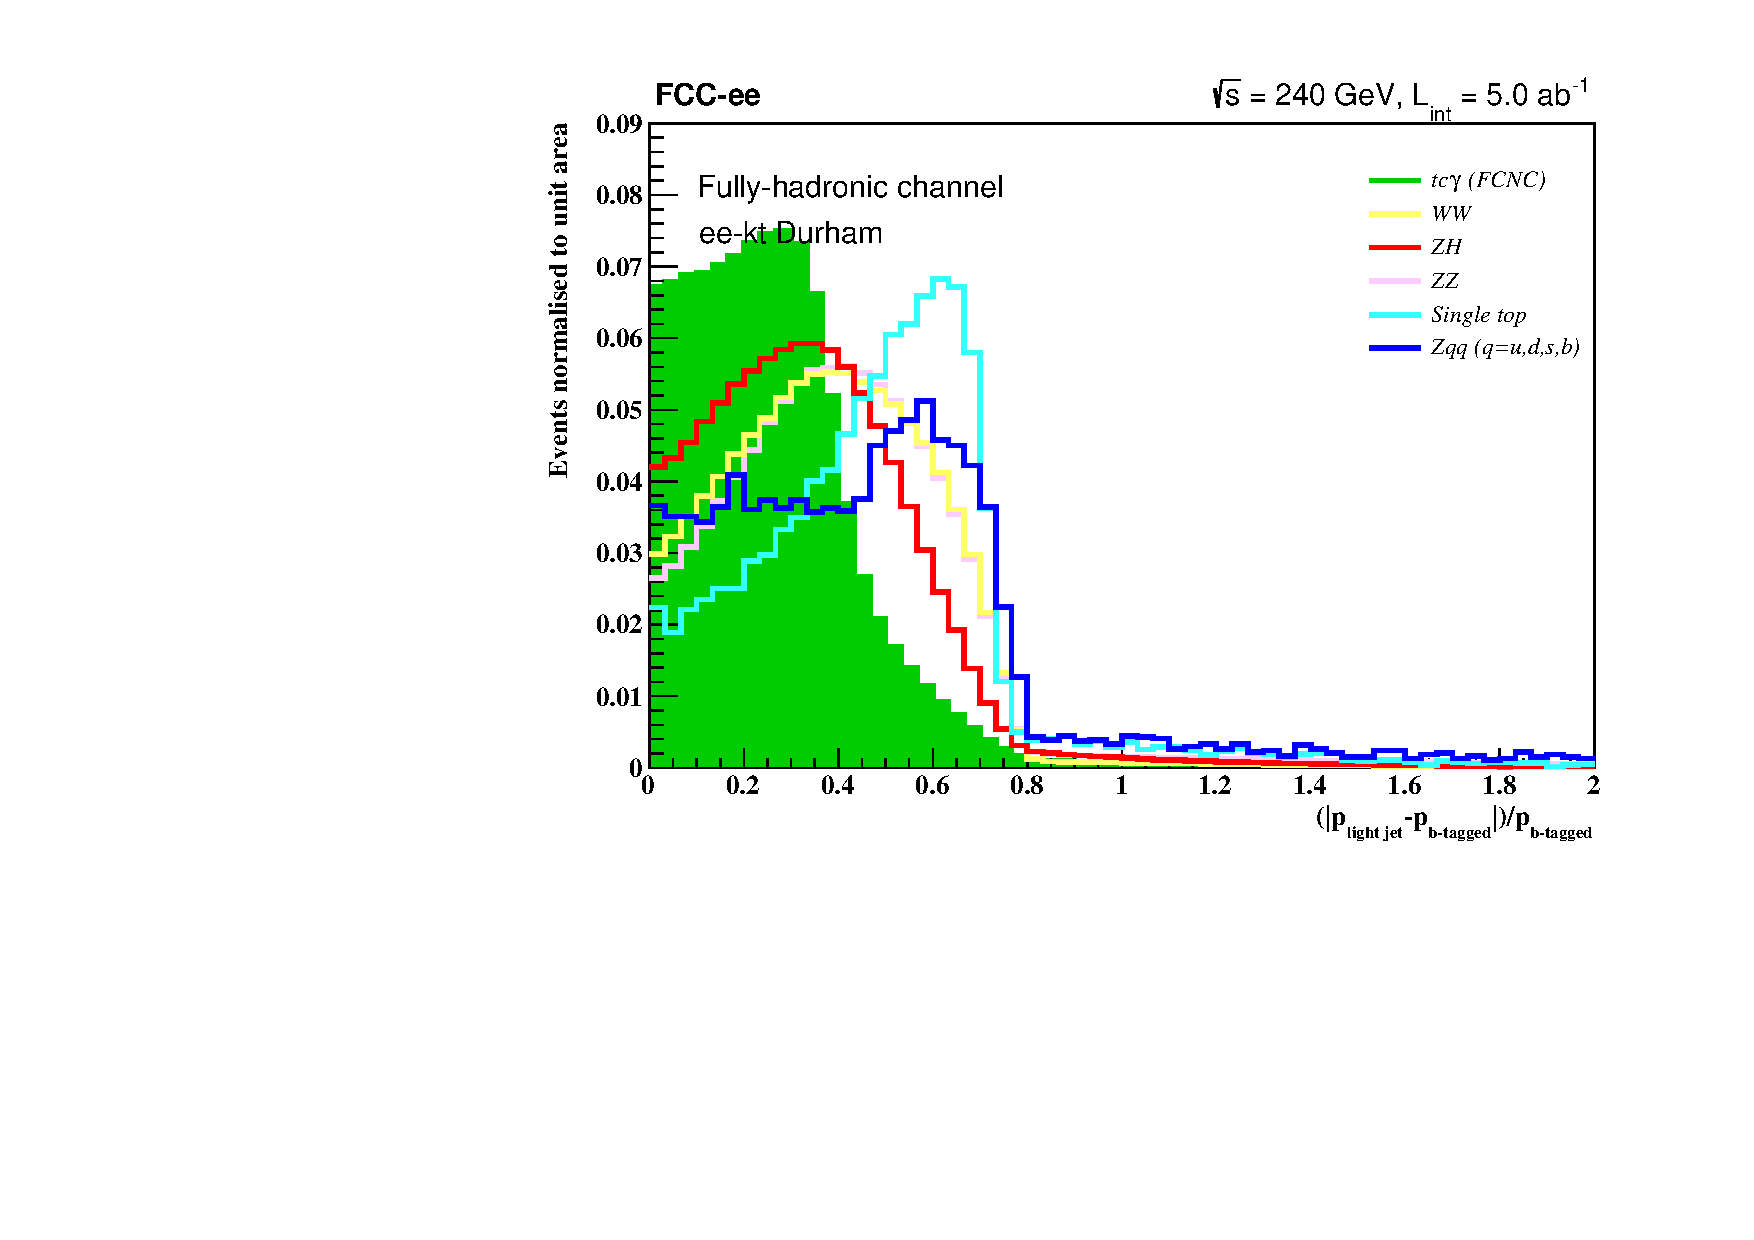
\includegraphics[width=0.45\textwidth]{240GeV-fullhadonic/dpp-full-240GeVs.pdf}} 	
\subfloat{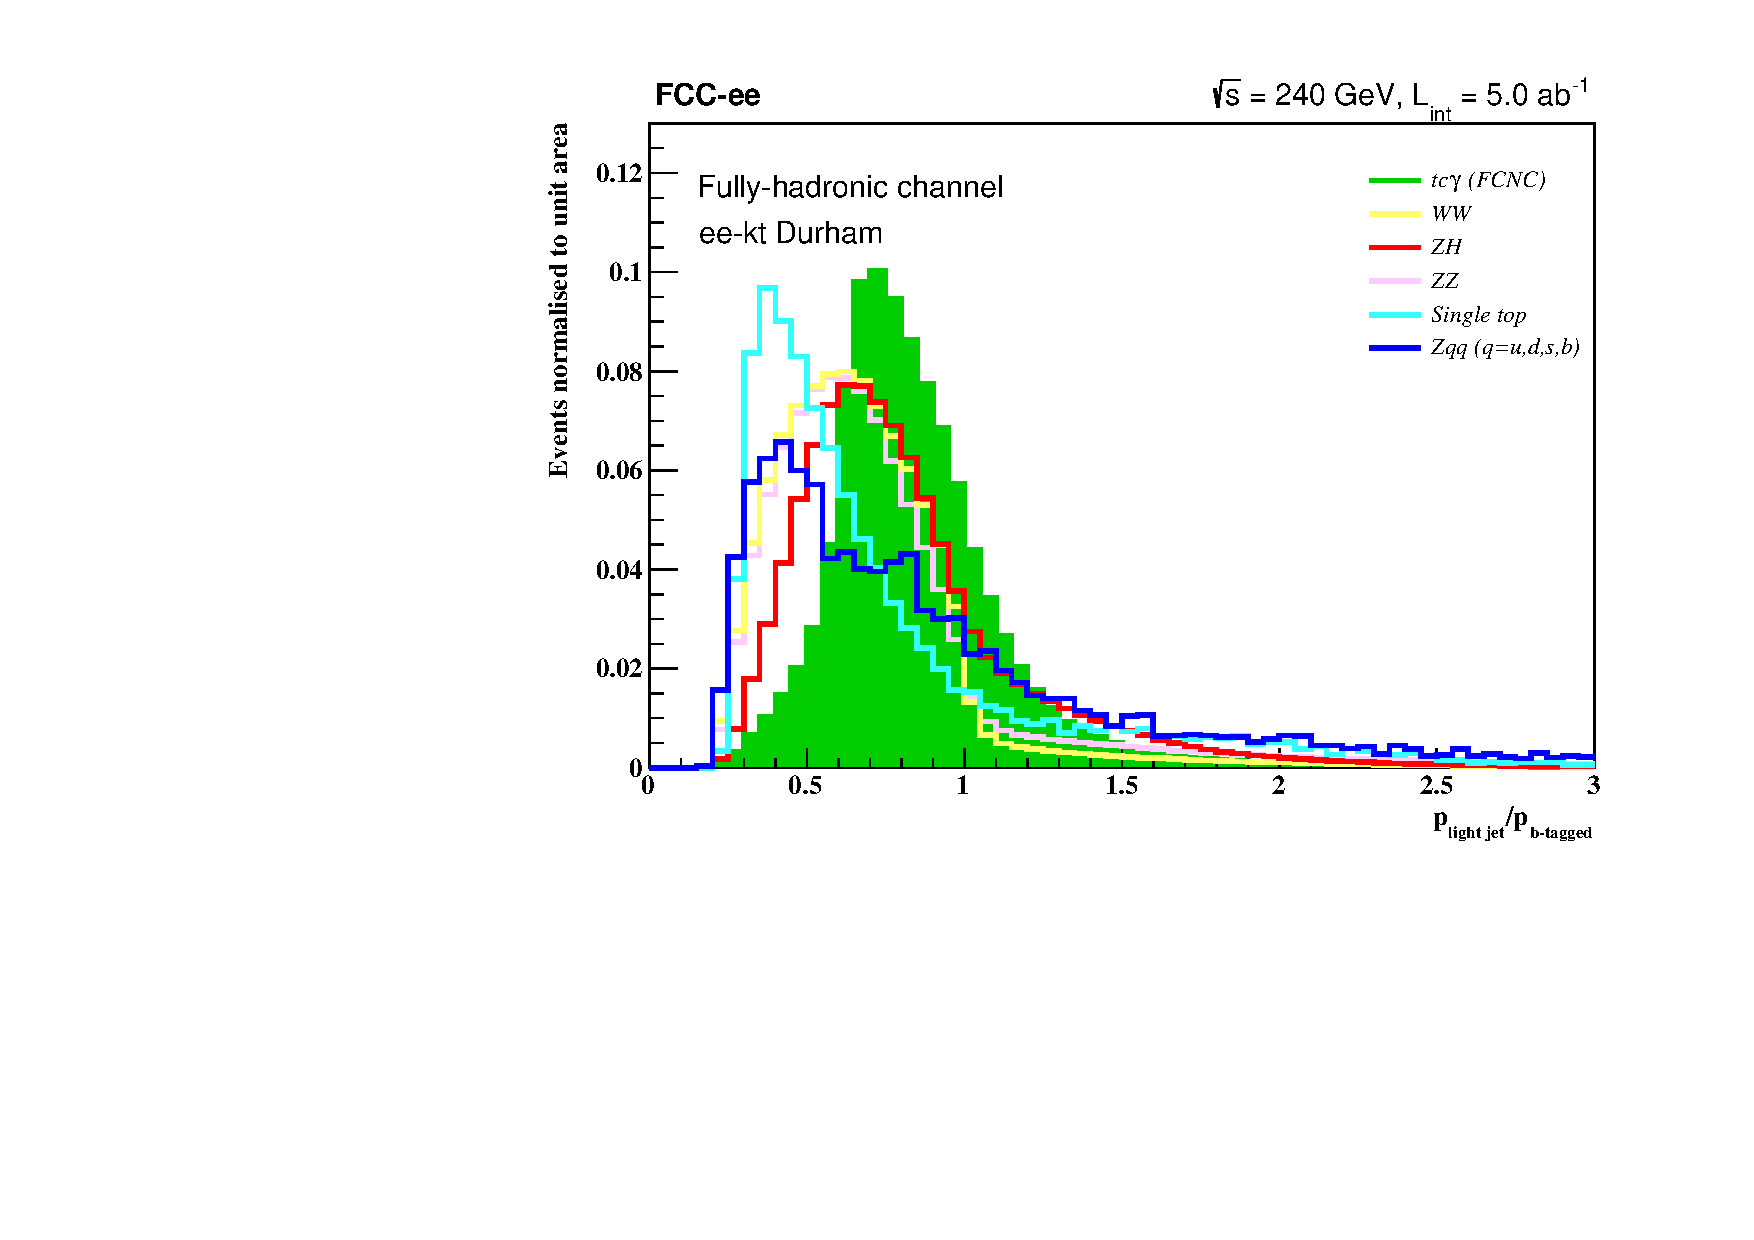
\includegraphics[width=0.45\textwidth]{240GeV-fullhadonic/plpb-full-240GeVs.pdf}}	
%\vspace{-6cm}
\begin{center}
\caption{ \small 
The distributions for the missing energy, the ratio of the total momentum of the light jet to the b-tagged jet, 
the ratio of the absolute value of momentum difference between the light jets and the b-tagged jets over  
the total momentum of the b-tagged jets, and the fake W boson mass distribution for the $\sqrt{s}= 240$ GeV. } 
\label{full-240GeV-2}
\end{center}
\end{figure*} 
%------------------------------------------------







%------------------------------------------------
\begin{figure*}[htb]
\vspace{0.50cm}
\centering
\subfloat{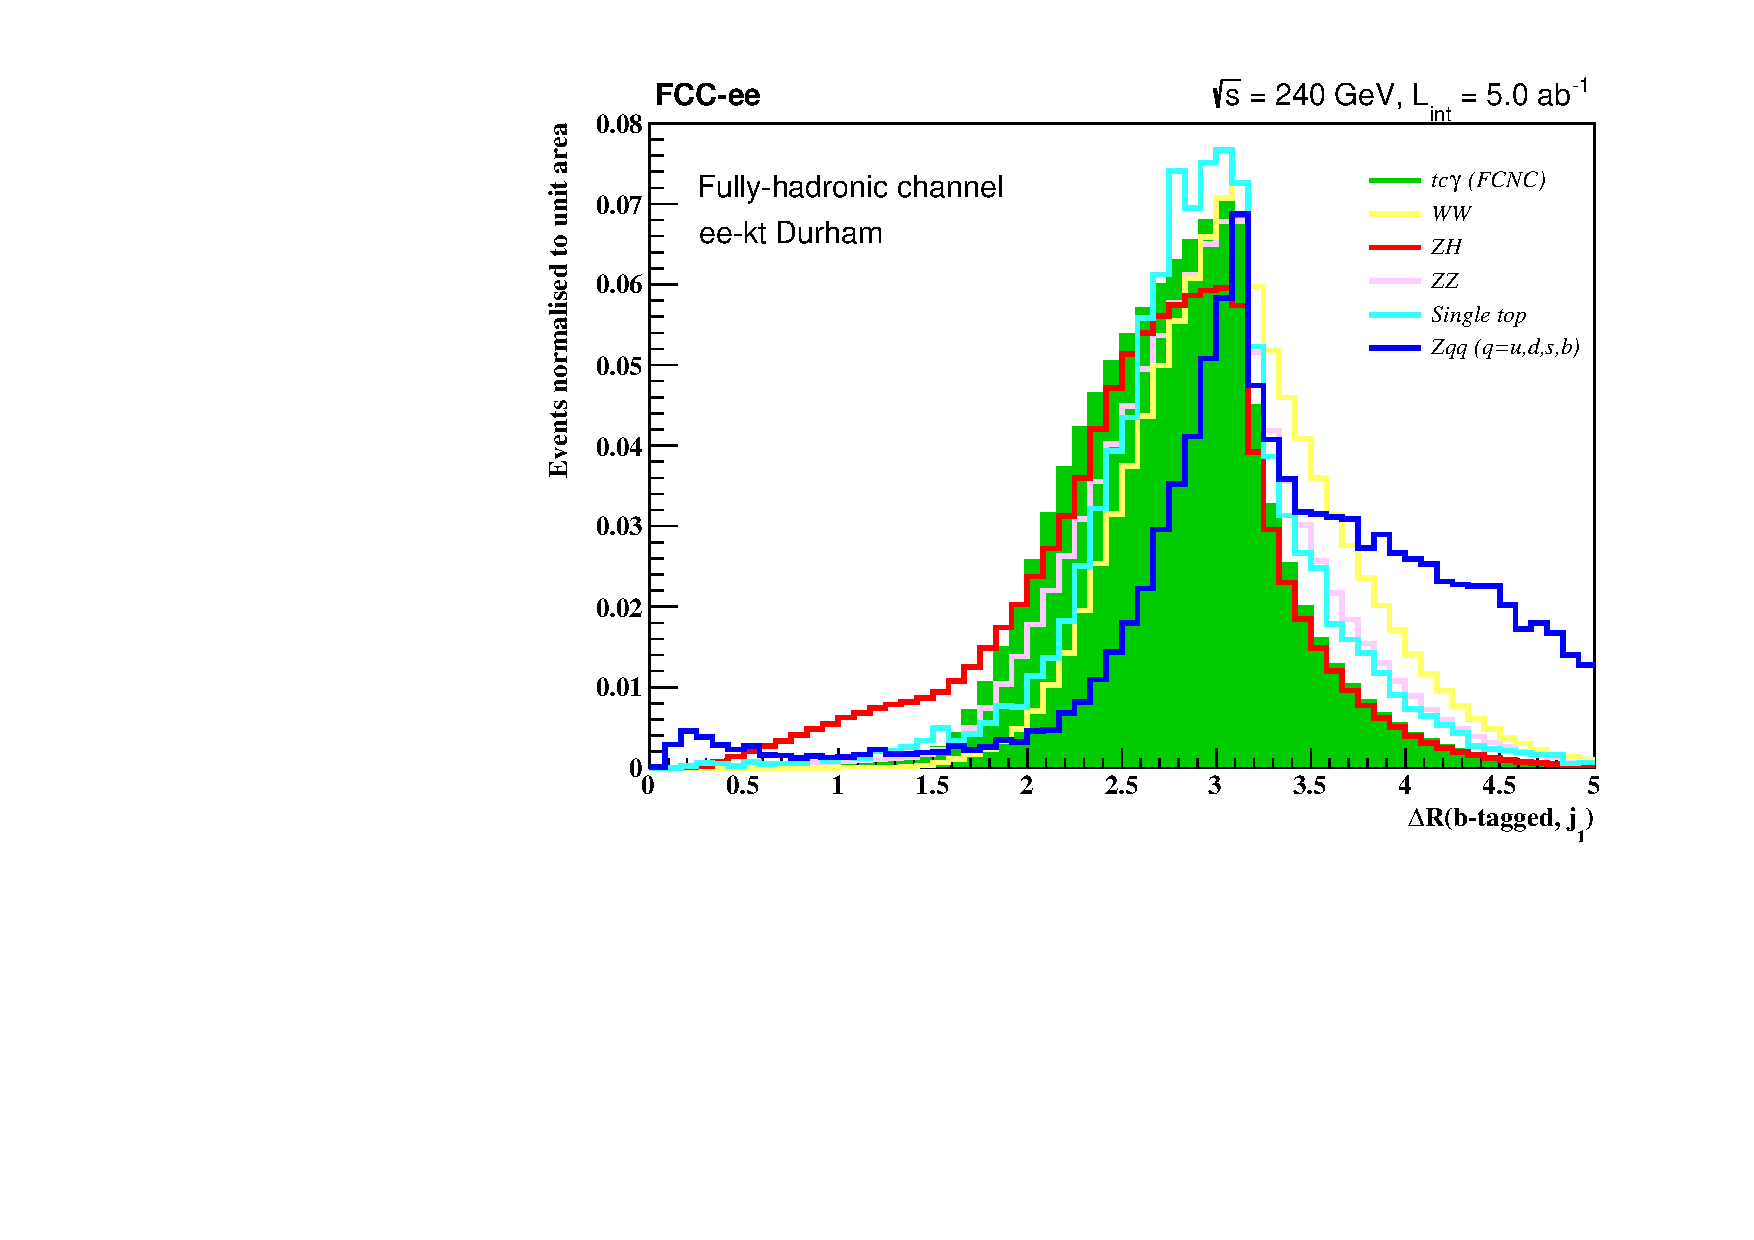
\includegraphics[width=0.45\textwidth]{240GeV-fullhadonic/drbjetjet1-full-240GeV.pdf}} 	
\subfloat{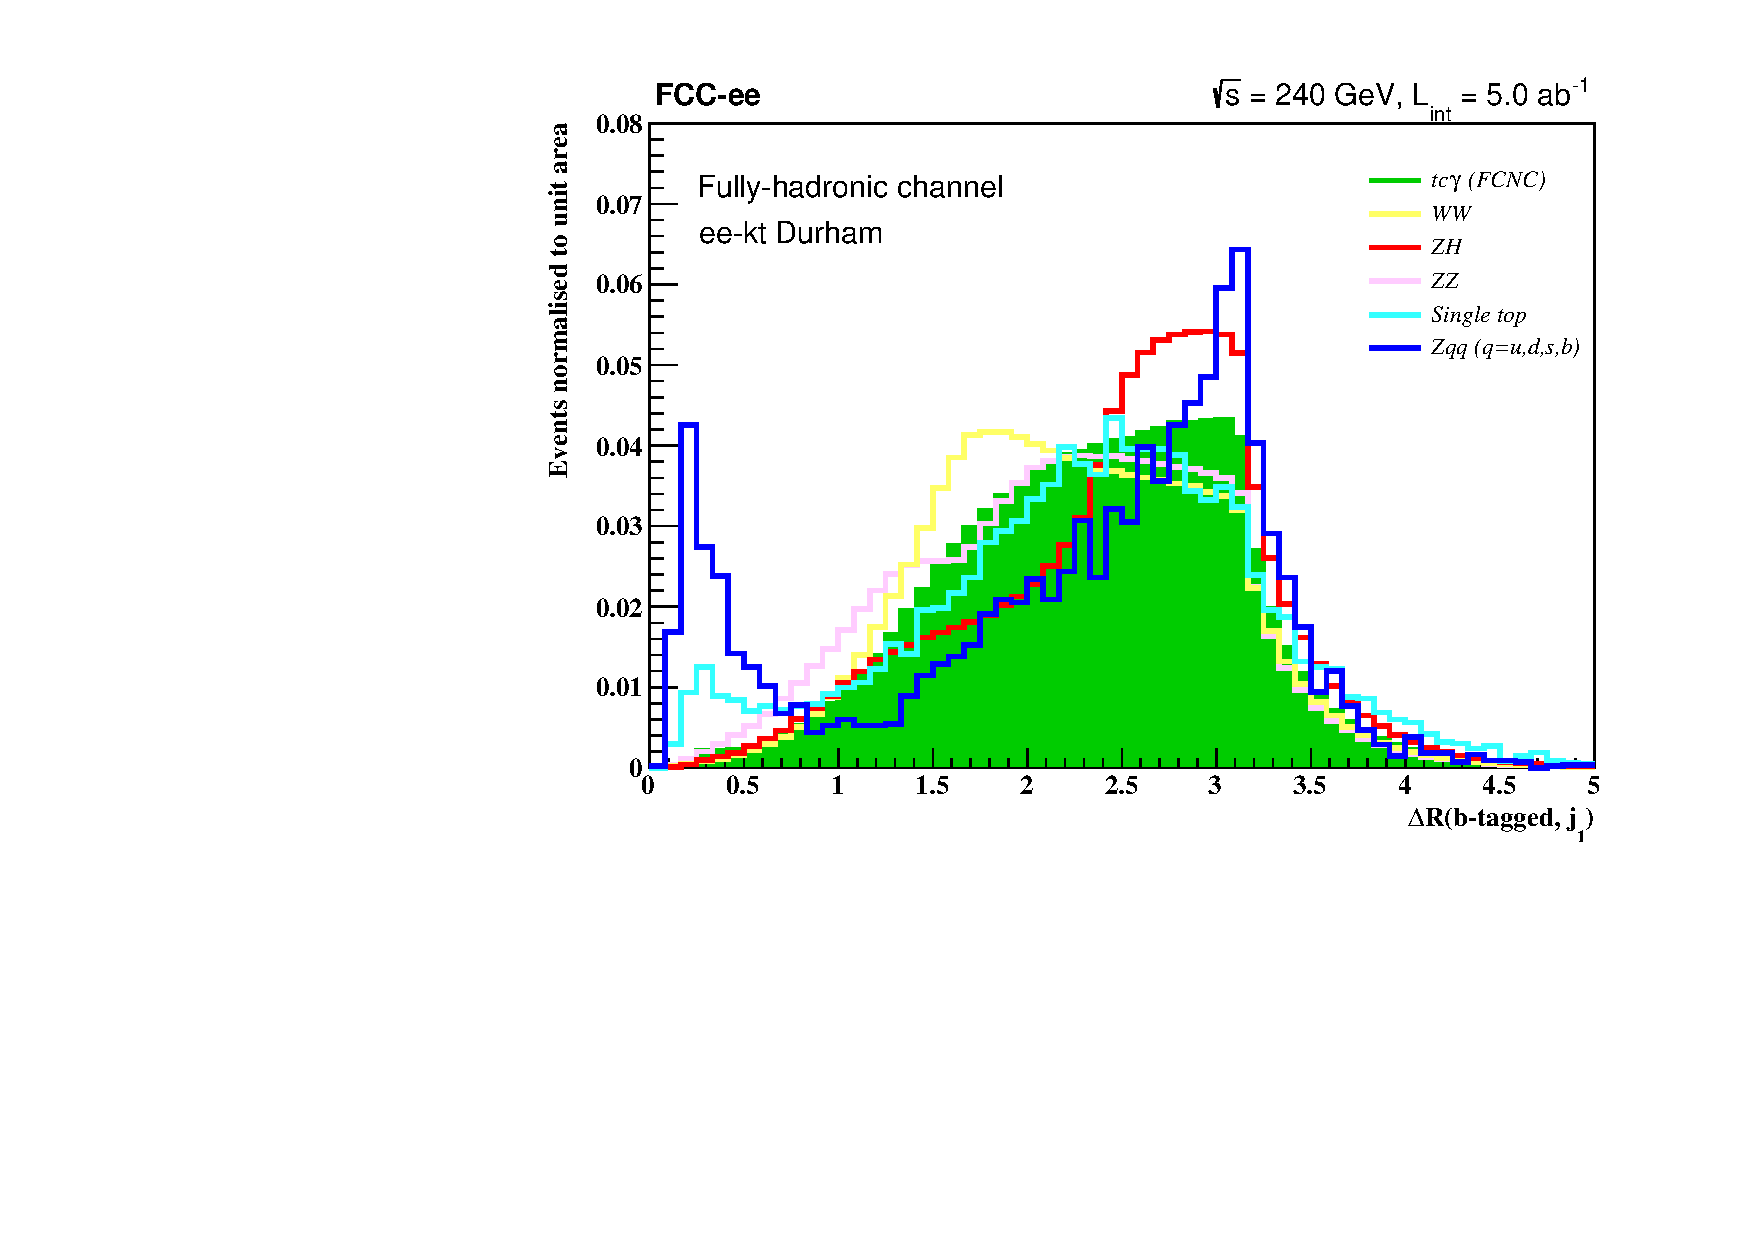
\includegraphics[width=0.45\textwidth]{240GeV-fullhadonic/drbjetjet2-full-240GeV.pdf}}	\\ 
\subfloat{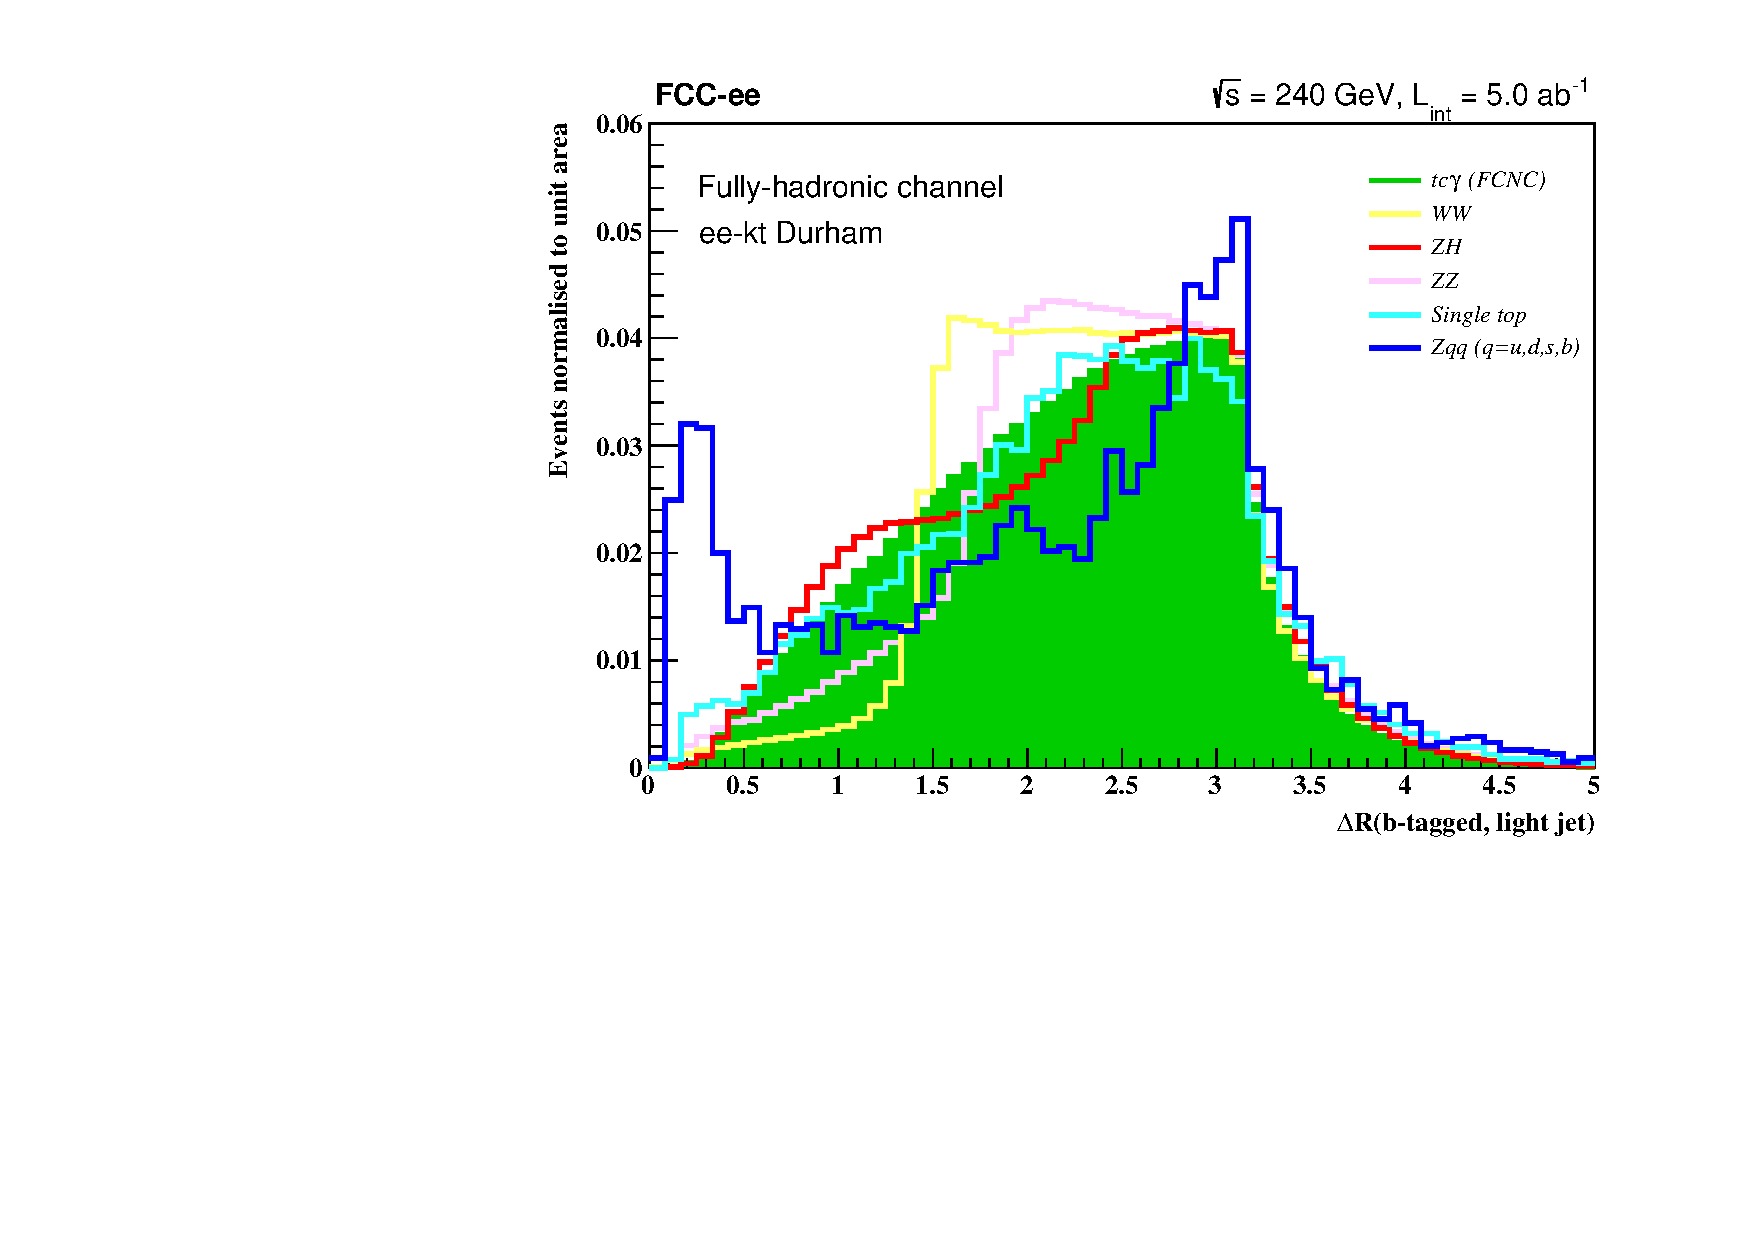
\includegraphics[width=0.45\textwidth]{240GeV-fullhadonic/drljetbjet-full-240GeV.pdf}} 	
\subfloat{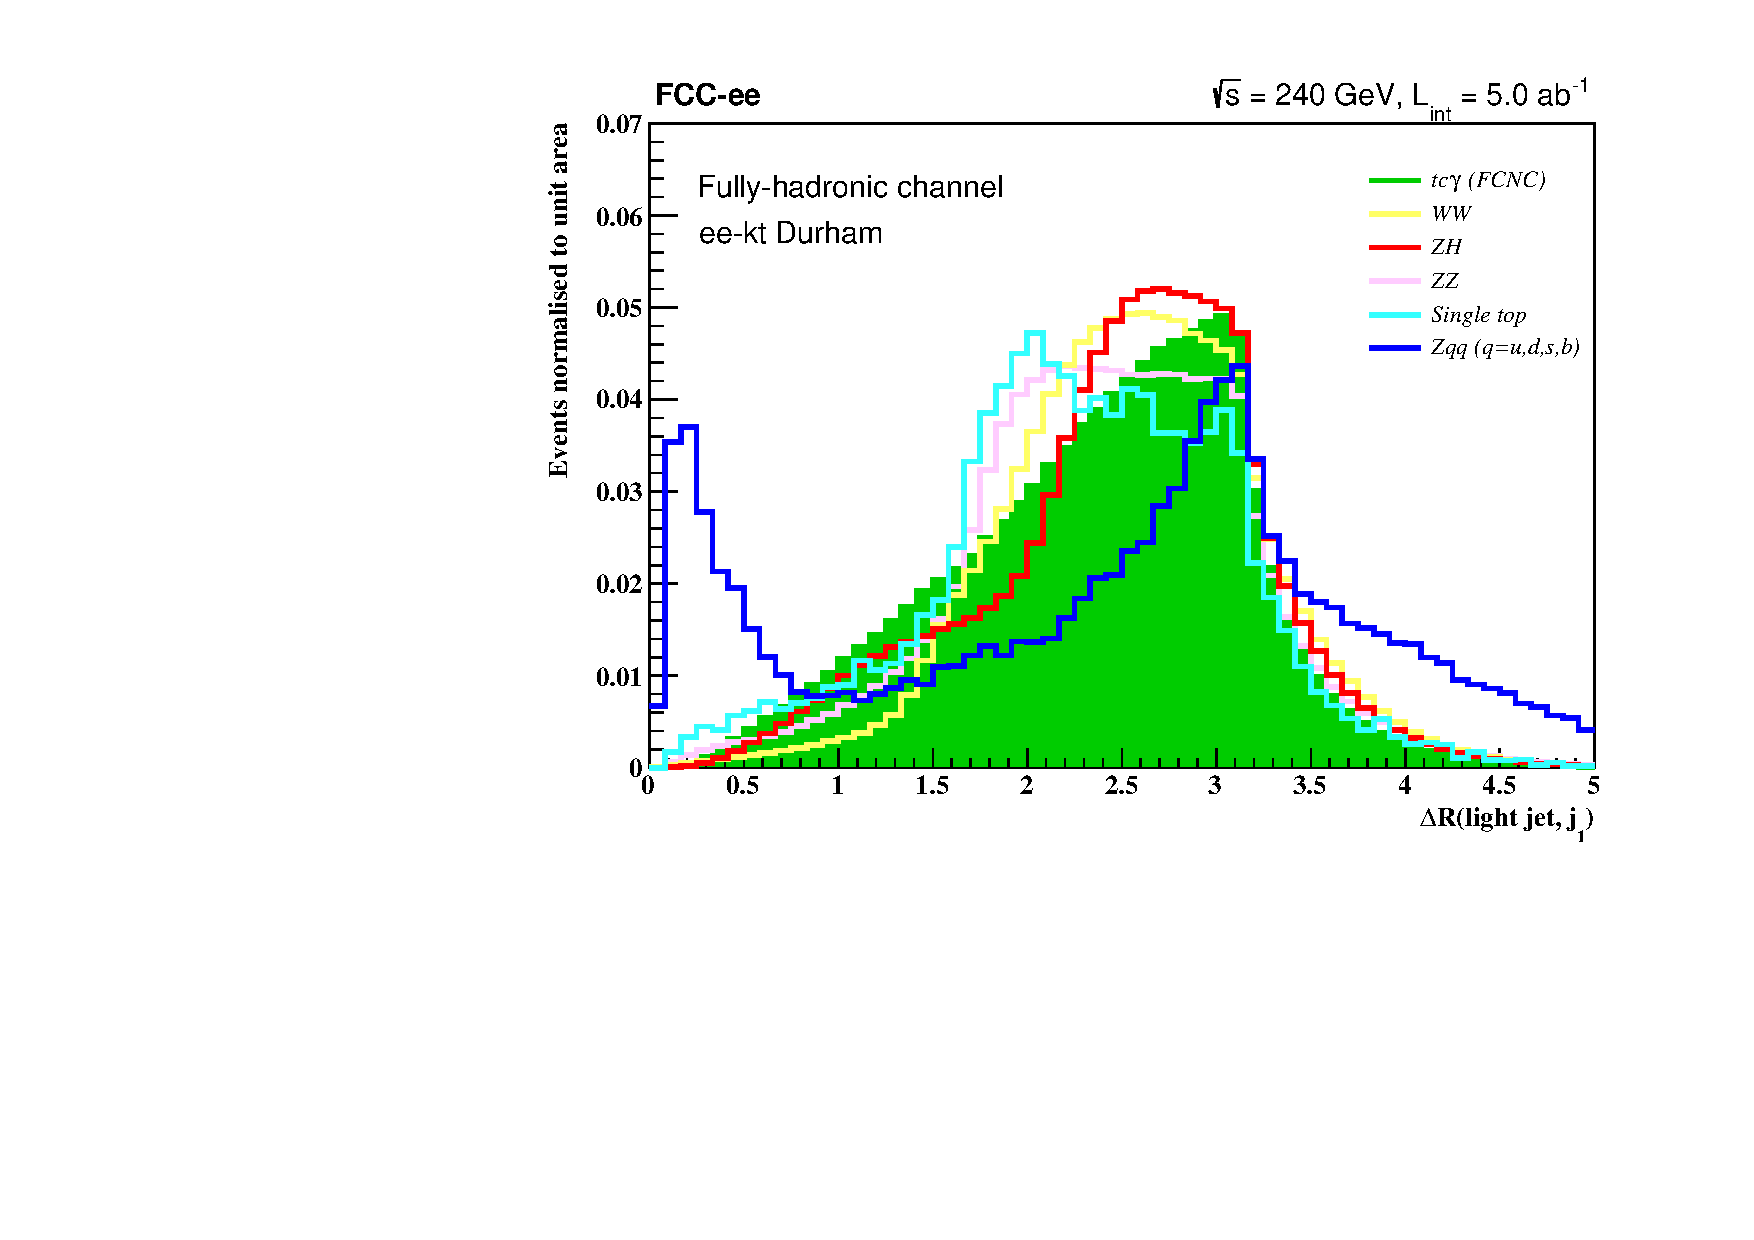
\includegraphics[width=0.45\textwidth]{240GeV-fullhadonic/drljetjet1-full-240GeV.pdf}}	
%\vspace{-6cm}
\begin{center}
\caption{ \small 
The angular separations between the jets (b-tagged and light jets) contributing
to the fully hadronic analysis at the $\sqrt{s}= 240$ GeV. }
\label{full-240GeV-3}
\end{center}
\end{figure*}
%------------------------------------------------
Based on the distribution presented above, we apply the following cuts to distinguish signals from backgrounds.
%======================
The final selection cuts for the fully hadronic analysis at a center-of-mass energy of 240 GeV are as follows:
\begin{itemize}
\item The reconstructed top-quark mass distribution: $150~\text{GeV} < M_{\text{top}} < 190~\text{GeV}$.
\item The reconstructed W boson mass distribution: $65~\text{GeV} < M_{\text{W}} < 95~\text{GeV}$.
\item The momentum of the $b$-jet candidate: $40~\text{GeV} < p_{\text{bjet}} < 95~\text{GeV}$.
\item The momentum of the highest energy light jet in each event: $p_{\text{lightjet}} > 50~\text{GeV}$.
\item The momentum of the first and second jets used to reconstruct the fake W boson: $40~\text{GeV} < p_{\text{j1}} < 90~\text{GeV}$ and $25~\text{GeV} < p_{\text{j2}} < 65~\text{GeV}$.
\item Missing Energy (ME): $ME > 10~\text{GeV}$.
\item The reconstructed invariant mass of the fake W boson: $M_{\text{W}} < 70~\text{GeV}$ or $M_{\text{W}} > 100~\text{GeV}$.
\item The maximum value of Missing Energy (ME): $ME < 10~\text{GeV}$.
\item Angular separations between the jets: $\Delta R(j, j_2) > 1$, $0.5 < \Delta R(\text{light-jet}, \text{b-jet}) < 4.0$, $0.7 < \Delta R(\text{light-jet}, j_2) < 4.0$, $1.6 < \Delta R(\text{b-jet}, j_1) < 3.5$, $0.8 < \Delta R(\text{b-jet}, j_2) < 4.0$, and $0.7 < \Delta R(\text{light-jet}, j_1) < 3.5$.
\item The ratio of the total momentum of the $b$-jet to the light jet: $0.60 < \frac{p_{\text{light-jet}}}{p_{\text{b-tagged}}} < 1.50$.
\item The ratio of the momentum of the $b$-jet to the sum of the $b$-jet and light jet momenta: $\frac{p_{\text{b-jet}}}{p_{\text{b-jet}}+p_{\text{light-jet}}} < 0.50$.
\item The scalar sum of momentum $H_T$: $H_T > 210~\text{GeV}$.
\end{itemize}
%======================

For the case of fully-hadronic analysis at 365 GeV, we consider the following
selection cuts: 

%======================
\begin{itemize}
\item Final selection cuts for the case of fully hadronic analysis at 240 GeV center-of-mass energy:
\begin{itemize}
\item The reconstructed top-quark mass distribution 150 GeV < $M_{\rm top}$ < 190 GeV.
\item The reconstructed W boson mass distribution  65 GeV < $M_{\rm W}$ < 95 GeV.
\item The momentum of $b$ jet candidate 35 GeV < $p_{\rm bjet}$ < 140 GeV.
\item The momentum of the highest energy light jet in each event 120 GeV <  $p_{\rm lightjet}$ < 150 GeV.
\item The momentum of the  first and second jets in each event that we use to reconstruct the fake W-boson, 
40 GeV <  $p_{\rm j1}$ < 140 GeV and $p_{\rm j2}$ > 80 GeV.
\item The Missing Energy ME > 10 GeV.   
\item The reconstructed invariant ass of fake W boson $M_{\rm W}$ > 100 GeV.
\item The maximum value of Missing Energy ME < 10 GeV.
\item The angular separation between the jets, i.e. $\Delta R(j, j_2)$ > 1; 1.0 < $\Delta R({light-jet}, b-jet)$ < 3.5; 
$0.7<\Delta R({light-jet}, j_2)$ < 3.5; 1.0<$\Delta R(b-jet, j_1)$ < 3.2; 0.5<$\Delta R(b-jet, j_2)$ < 3.5;  $1.7<\Delta R({light-jet}, j_1) < 3.5$.
%\item The ratio of total momentum of $b$-jet to light jet, $0.50 < \frac{p_{light jet}}{p_{b-tagged}} < 1.5$.
\item The scalar sum of momentum $H_T$ > 330 GeV.
\item The total momentum of reconstructed top-quark, 110 GeV < $p^{\rm top}$ < 150 GeV.
\end{itemize}
\end{itemize}
%======================
  
After applying the typical pre-selection and final-selection cuts mentioned above, we present the cross sections for the considered backgrounds at center-of-mass energies of 240 GeV and 365 GeV in Table~\ref{bkg-240-full-hadronic} and Table~\ref{bkg-365-full-hadronic}, respectively.
%======================
\begin{table*}[htbp]
\begin{center}
\begin{tabular}{l|c c c c c c  c c c c c  }  \hline
$\sqrt {s}$ = 240 GeV   ~&~ $tc\gamma$  ~&~ $tcZ$   ~&  ~  ZH     ~&  ~ WW  &  ~  ZZ ~ &~ eebb ~&~ eeqq (q=uds) ~&~ single top  \\  \hline
Cross section (fb)    ~&~  $28.39$  ~&~ $67.44$  ~&~    $201.868$        ~&~  $16438.5$   ~&~    $1358.99$  ~&~  $455.7$ ~&~  $1635.9$  ~&~  $0.01075$       \\ 
Preselection    ~&~  $22.571$  & $38.651$  &    $83.452$        &  $4285.272$   &    $400.682$  &  $0.2511$ &  $1.3863$  &  $0.00082$        \\ 
Final selection
  &  $6.609$  & $11.320$  &    $8.361$        &  $257.030$   &    $34.193$  &  $0.00018$ &  $0.0027$  &  $4.83\times10^{-7}$       \\   \hline  \hline
\end{tabular}
\end{center}
\caption{Cross-sections in the unit of fb for the signal scenario with fully hadronic decay  
and for the main SM backgrounds considered in this study 
passing pre-selection and final selection cuts at a center-of-mass energy of 240 GeV.}
\label{bkg-240-full-hadronic}
\end{table*}
%======================


%======================
\begin{table*}[htbp]
\begin{center}
\begin{tabular}{l|c c c c  c c  c c c c c  }  \hline
$\sqrt {s}$ = 365 GeV      & $tc\gamma$  & $tcZ$   & ZH   &  WW  & ZZ & $t \bar{t}$ & eebb & single top & $tbjj$  \\  \hline
Cross section (fb)    ~&~  $52.39$  ~&~  $104.0$    ~&~  $117.3$ ~&~    $10716.5$     ~&~  $642.8$  ~&~ $800.0$        ~&~  $615.2$  ~&~  $0.227$  ~&~ $5.98$       \\ 
Preselection    ~&~  $39.152$  ~&~  $76.435$    ~&~  $32.779$ ~&~  $2137.639$     ~&~  $0.2038$  ~&~ $271.443$    ~&~  $0.1626$  ~&~  $0.0034$  ~&~ $2.973$       \\ 
Final selection    ~&~  $14.499$  ~&~  $28.318$    ~&~  $2.194$ ~&~ $52.307$  ~&~  $5.775$  ~&~ $5.689$  ~&~  $8.66 \times 10^{-5}$  ~&~ $\sim 0$  ~&~ $0.055$       \\  \hline  \hline
\end{tabular}
\end{center}
\caption{Same as Table.~\ref{bkg-240-full-hadronic} but this time for the center-of-mass energy of 365 GeV.}
\label{bkg-365-full-hadronic}
\end{table*}
%======================



\clearpage



%---------------------------------------------
\subsection{Results for the fully hadronic analysis}
%---------------------------------------------
The primary results and findings from the fully hadronic analysis conducted at both 240 GeV and 365 GeV center-of-mass energies are highlighted in this section.
Using the CL$s$ method, the upper limits at the $95\%$ confidence level (CL) for the top FCNC decays at a center-of-mass energy of $\sqrt{s} = 240$ GeV are determined. These limits are summarized in Table \ref{limits-240-full}. These limits correspond to the FCC-ee operating with an integrated luminosity of 5 ab$^{-1}$ at a center-of-mass energy of $\sqrt{s} = 240$ GeV. The corresponding values for $\sqrt{s} = 365$ GeV, along with an integrated luminosity of 1.5 ab$^{-1}$, are provided in Table \ref{limits-365-full}.

%======================
\begin{table*}[htbp]
\begin{center}
\begin{tabular}{l|c c c c }  \hline
$\sqrt {s}$ = 240 GeV  &  ~  $Br (t \to c \gamma )$       &  ~ $Br (t \to c Z)$      \\  \hline
Full hadronic decay            &  ~  $1.98  \times 10^{-4}$        & ~ $1.01 \times 10^{-4}$     \\   \hline  \hline
\end{tabular}
\end{center}
\caption{The upper limits on the top FCNC decays for the fully hadronic decay analysis  
at $95\%$ C.L obtained using the CL$s$ method
at the $\sqrt {s}$ = 240 GeV and for an integrated luminosity of 5 ab$^{-1}$.}
\label{limits-240-full}
\end{table*}
%======================




%======================
\begin{table*}[htbp]
\begin{center}
\begin{tabular}{l|c c c c }  \hline
$\sqrt {s}$ = 365 GeV  &  ~  $Br (t \to c \gamma )$       &  ~ $Br (t \to c Z)$      \\  \hline
Full hadronic decay           &  ~  $8.45  \times 10^{-5}$        & ~ $3.70  \times 10^{-5}$    \\   \hline  \hline
\end{tabular}
\end{center}
\caption{Same as Table.~\ref{limits-240}, but this time for the 
$\sqrt {s}$ = 365 GeV and for an integrated luminosity of 1.5 ab$^{-1}$.}
\label{limits-365-full}
\end{table*}
%======================





%
%%%%%%%%%%%%%%%%%%%%%%%%%%%%%%%%%%%%%%%%%%%%%%%%%%%%%%%%%%%%%%%%%%%%%%%
\subsection{Statistical combination of results in hadronic channel}\label{Combination-hadronic}     
%%%%%%%%%%%%%%%%%%%%%%%%%%%%%%%%%%%%%%%%%%%%%%%%%%%%%%%%%%%%%%%%%%%%%%%
%


In Table.~\ref{limits-combination-hadronic}, the upper limits on the top FCNC     
decays at $95\%$ C.L extracted using 
the {\tt Higgs Combine Tool}~\cite{Higgs-Combination-Tool} after the statistical combination of $\sqrt {s}$ = 240 and 365 GeV are presented. 



%======================
\begin{table*}[htbp]
\begin{center}
\begin{tabular}{l|c c c c }  \hline
$\sqrt {s}$ = 240 and 365 GeV  &  ~  $Br (t \to c \gamma )$    ~&  ~ $Br (t \to c Z)$      \\  \hline
 Statistical combination   &  ~  $ 7.65 \times 10^{-5}$          ~ & ~ $ 3.28 \times 10^{-5}$        \\   \hline  \hline  
\end{tabular}
\end{center}
\caption{The upper limits on the top FCNC decays at $95\%$ C.L obtained using the Higgs combination 
tools after combination of $\sqrt {s}$ = 240 and 365 GeV. }   
\label{limits-combination-hadronic}
\end{table*}
%======================



%
%%%%%%%%%%%%%%%%%%%%%%%%%%%%%%%%%%%%%%%%%%%%%%%%%%%%%%%%%%%%%%%%%%%%%%%
\section{Discussion and Conclusion}\label{Conclusion}
%%%%%%%%%%%%%%%%%%%%%%%%%%%%%%%%%%%%%%%%%%%%%%%%%%%%%%%%%%%%%%%%%%%%%%%
%

It is anticipated that the future high-energy and high-luminosity collider, FCC-ee, with its clean environment and high luminosity, will offer a unique opportunity to accurately measure the properties of top quarks and their interactions. In this study, we investigated the potential sensitivity of FCC-ee to flavor-changing neutral current (FCNC) transitions involving top quarks.
Specifically, we focused on the $tqZ$ and $tq\gamma$ couplings, where $q=u, c$. To ensure model independence, we employed the effective Lagrangian approach and examined the single top-quark production process in $e^- e^+$ collisions, specifically $e^- e^+ \to \bar{t} q + t \bar{q}$. Our analysis considered both leptonic decays (electron and muon) and fully hadronic decays of the W boson in the top quark decay.
To conduct our study, we utilized the official FCCAnalysis framework and employed various jet clustering algorithms. We generated FCNC signal and background samples using the IDEA detector response, and also generated samples in the EDM4HEP format.
Through our analysis, we demonstrated that by combining energy and channels, and considering integrated luminosities of 5 and 1.5 ab$^{-1}$, we could achieve sensitivity on the order of $10^{-5}$ to $10^{-6}$.



%
%%%%%%%%%%%%%%%%%%%%%%%%%%%%%%%%%%%%%%%%%%%%%%%%%%%%%%%%%%%%%%%%%%%%%%%
\begin{acknowledgments}
%%%%%%%%%%%%%%%%%%%%%%%%%%%%%%%%%%%%%%%%%%%%%%%%%%%%%%%%%%%%%%%%%%%%%%%
%


The authors would like to express their gratitude for the valuable discussions 
and helpful comments received from  FCC-ee Collaboration.  


%
%%%%%%%%%%%%%%%%%%%%%%%%%%%%%%%%%%%%%%%%%%%%%%%%%%%%%%%%%%%%%%%%%%%%%%%
\end{acknowledgments}
%%%%%%%%%%%%%%%%%%%%%%%%%%%%%%%%%%%%%%%%%%%%%%%%%%%%%%%%%%%%%%%%%%%%%%%
%
	
	







%%%%%%%%%%%%%%%%%%%%%%%%%%%%%%%%
%
% BibTeX users please use
% \bibliographystyle{}
% \bibliography{}
%
% Non-BibTeX users please use



\clearpage


%%%%%%%%%%%%%%%%%%%%%%%%%%%%%%%%
\begin{thebibliography}{}
%%%%%%%%%%%%%%%%%%%%%%%%%%%%%%%%
	


%\cite{CDF:1995wbb}
\bibitem{CDF:1995wbb}
F.~Abe \textit{et al.} [CDF],
``Observation of top quark production in $\bar{p}p$ collisions,''
Phys. Rev. Lett. \textbf{74}, 2626-2631 (1995)
doi:10.1103/PhysRevLett.74.2626
[arXiv:hep-ex/9503002 [hep-ex]].
%3973 citations counted in INSPIRE as of 08 Dec 2022




%\cite{D0:1995jca}
\bibitem{D0:1995jca}
S.~Abachi \textit{et al.} [D0],
``Observation of the top quark,''
Phys. Rev. Lett. \textbf{74}, 2632-2637 (1995)
doi:10.1103/PhysRevLett.74.2632
[arXiv:hep-ex/9503003 [hep-ex]].
%3389 citations counted in INSPIRE as of 08 Dec 2022





%\cite{Glashow:1970gm}
\bibitem{Glashow:1970gm}
S.~L.~Glashow, J.~Iliopoulos and L.~Maiani,
``Weak Interactions with Lepton-Hadron Symmetry,''
Phys. Rev. D \textbf{2}, 1285-1292 (1970)
doi:10.1103/PhysRevD.2.1285
%6547 citations counted in INSPIRE as of 15 Jan 2023
	



%\cite{Aguilar-Saavedra:2004mfd}
\bibitem{Aguilar-Saavedra:2004mfd}
J.~A.~Aguilar-Saavedra,
``Top flavor-changing neutral interactions: Theoretical expectations and experimental detection,''
Acta Phys. Polon. B \textbf{35}, 2695-2710 (2004)
[arXiv:hep-ph/0409342 [hep-ph]].
%399 citations counted in INSPIRE as of 15 Jan 2023




%\cite{Aguilar-Saavedra:2008nuh}
\bibitem{Aguilar-Saavedra:2008nuh}
J.~A.~Aguilar-Saavedra,
``A Minimal set of top anomalous couplings,''
Nucl. Phys. B \textbf{812}, 181-204 (2009)
doi:10.1016/j.nuclphysb.2008.12.012
[arXiv:0811.3842 [hep-ph]].
%399 citations counted in INSPIRE as of 15 Jan 2023
	






%\cite{Alloul:2013bka}
\bibitem{Alloul:2013bka}
A.~Alloul, N.~D.~Christensen, C.~Degrande, C.~Duhr and B.~Fuks,
``FeynRules  2.0 - A complete toolbox for tree-level phenomenology,''
Comput. Phys. Commun. \textbf{185}, 2250-2300 (2014),
%doi:10.1016/j.cpc.2014.04.012
[arXiv:1310.1921 [hep-ph]].
%2148 citations counted in INSPIRE as of 12 Apr 2023




%\cite{Duhr:2011se}
\bibitem{Duhr:2011se}
C.~Duhr and B.~Fuks,
``A superspace module for the FeynRules package,''
Comput. Phys. Commun. \textbf{182}, 2404-2426 (2011),
%doi:10.1016/j.cpc.2011.06.009
[arXiv:1102.4191 [hep-ph]].
%87 citations counted in INSPIRE as of 12 Apr 2023






%\cite{Christensen:2009jx}
\bibitem{Christensen:2009jx}
N.~D.~Christensen, P.~de Aquino, C.~Degrande, C.~Duhr, B.~Fuks, M.~Herquet, F.~Maltoni and S.~Schumann,
``A Comprehensive approach to new physics simulations,''
Eur. Phys. J. C \textbf{71}, 1541 (2011),
%doi:10.1140/epjc/s10052-011-1541-5
[arXiv:0906.2474 [hep-ph]].
%181 citations counted in INSPIRE as of 12 Apr 2023





%\cite{Degrande:2011ua}
\bibitem{Degrande:2011ua}
C.~Degrande, C.~Duhr, B.~Fuks, D.~Grellscheid, O.~Mattelaer and T.~Reiter,
``UFO - The Universal FeynRules Output,''
Comput. Phys. Commun. \textbf{183}, 1201-1214 (2012),
%doi:10.1016/j.cpc.2012.01.022
[arXiv:1108.2040 [hep-ph]].
%1146 citations counted in INSPIRE as of 12 Apr 2023








%\cite{Mrenna:2016sih}
\bibitem{Mrenna:2016sih}
S.~Mrenna and P.~Skands,
%``Automated Parton-Shower Variations in Pythia 8,''
Phys. Rev. D \textbf{94}, no.7, 074005 (2016)
doi:10.1103/PhysRevD.94.074005
[arXiv:1605.08352 [hep-ph]].
%93 citations counted in INSPIRE as of 12 Apr 2023




%\cite{deFavereau:2013fsa}
\bibitem{deFavereau:2013fsa}
J.~de Favereau \textit{et al.} [DELPHES 3],
%``DELPHES 3, A modular framework for fast simulation of a generic collider experiment,''
JHEP \textbf{02}, 057 (2014)
doi:10.1007/JHEP02(2014)057
[arXiv:1307.6346 [hep-ex]].
%2541 citations counted in INSPIRE as of 12 Apr 2023






%\cite{FCC-ee-IDEA-detector}
\bibitem{FCC-ee-IDEA-detector}
FCC-ee IDEA detector model, Elisa Fontanesi, Lorenzo Pezzotti, Massimiliano Antonello, Michele Selvaggi,
https://indico.cern.ch/event/1173562/contributions/\\4929025/attachments/2470068/4237859/2022-06-FCC-jets.pdf

	






%\cite{Catani:1991hj}
\bibitem{Catani:1991hj}
S.~Catani, Y.~L.~Dokshitzer, M.~Olsson, G.~Turnock and B.~R.~Webber,
``New clustering algorithm for multi - jet cross-sections in e+ e- annihilation,''
Phys. Lett. B \textbf{269}, 432-438 (1991),
%doi:10.1016/0370-2693(91)90196-W
%1365 citations counted in INSPIRE as of 08 Apr 2023





%\cite{Lai:2021rko}
\bibitem{Lai:2021rko}
P.~Z.~Lai, M.~Ruan and C.~M.~Kuo,
``Jet performance at the circular electron-positron collider,''
JINST \textbf{16}, no.07, P07037 (2021),
%doi:10.1088/1748-0221/16/07/P07037
[arXiv:2104.05029 [hep-ex]].
%5 citations counted in INSPIRE as of 08 Apr 2023







%\cite{Bedeschi:2022rnj}
\bibitem{Bedeschi:2022rnj}
F.~Bedeschi, L.~Gouskos and M.~Selvaggi,
``Jet flavour tagging for future colliders with fast simulation,''
Eur. Phys. J. C \textbf{82}, no.7, 646 (2022),
%doi:10.1140/epjc/s10052-022-10609-1
[arXiv:2202.03285 [hep-ex]].
%7 citations counted in INSPIRE as of 05 Apr 2023




%\cite{Aguilar-Saavedra:2004mfd}
\bibitem{Aguilar-Saavedra:2004mfd}
J.~A.~Aguilar-Saavedra,
``Top flavor-changing neutral interactions: Theoretical expectations and experimental detection,''
Acta Phys. Polon. B \textbf{35}, 2695-2710 (2004),
%[arXiv:hep-ph/0409342 [hep-ph]].
%411 citations counted in INSPIRE as of 10 Aug 2023




%\cite{Aguilar-Saavedra:2008nuh}
\bibitem{Aguilar-Saavedra:2008nuh}
J.~A.~Aguilar-Saavedra,
``A Minimal set of top anomalous couplings,''
Nucl. Phys. B \textbf{812}, 181-204 (2009),
%doi:10.1016/j.nuclphysb.2008.12.012
[arXiv:0811.3842 [hep-ph]].
%408 citations counted in INSPIRE as of 10 Aug 2023



%\cite{Aguilar-Saavedra:2009ygx}
\bibitem{Aguilar-Saavedra:2009ygx}
J.~A.~Aguilar-Saavedra,
``A Minimal set of top-Higgs anomalous couplings,''
Nucl. Phys. B \textbf{821}, 215-227 (2009),
%doi:10.1016/j.nuclphysb.2009.06.022
[arXiv:0904.2387 [hep-ph]].
%187 citations counted in INSPIRE as of 10 Aug 2023





%\cite{Tenchini}
\bibitem{Tenchini}
%\label{Tenchini}
R.~Tenchini and C.~Verzegnassi, \textit{The Physics of the W and Z Bosons}, World Scientific, 2007.





%\cite{Higgs-Combination-Tool}
\bibitem{Higgs-Combination-Tool}
%\label{Tenchini}
https://cms-analysis.github.io/HiggsAnalysis-CombinedLimit/





	
\end{thebibliography}
%

\end{document}

